%%%%%%%%%%%%%%%%%%%%%%%%%%%%%%%%%%%%%%%%%%%%%%%%%%%%%%%%%%%%%%%%%%%%%%%%%%%%%
%%% LaTeX-Rahmen fuer das Erstellen von Bachelorarbeiten
%%%%%%%%%%%%%%%%%%%%%%%%%%%%%%%%%%%%%%%%%%%%%%%%%%%%%%%%%%%%%%%%%%%%%%%%%%%%%

%%%%%%%%%%%%%%%%%%%%%%%%%%%%%%%%%%%%%%%%%%%%%%%%%%%%%%%%%%%%%%%%%%%%%%%%%%%%%
%%% allgemeine Einstellungen
%%%%%%%%%%%%%%%%%%%%%%%%%%%%%%%%%%%%%%%%%%%%%%%%%%%%%%%%%%%%%%%%%%%%%%%%%%%%%

\documentclass[twoside,10pt,a4paper]{report}
\usepackage[utf8]{inputenc}
\usepackage[T1]{fontenc}

\usepackage{graphics, graphicx}
\usepackage{latexsym}
\usepackage[margin=10pt,font=small,labelfont=bf]{caption}



\usepackage[section]{placeins}
\usepackage{multirow}
\usepackage[table]{xcolor}
\usepackage{bussproofs}
\usepackage{tabu}
\usepackage{csquotes}
\usepackage{amsmath}
\usepackage{subcaption}
\usepackage{geometry}
\usepackage{mathpartir}
\usepackage{listings}
\usepackage{mathtools}
\usepackage{amssymb}
\usepackage{tikz}
\usetikzlibrary{positioning, calc, arrows, tikzmark}
\usetikzlibrary{shapes.multipart}
\usepackage{xcolor}
\definecolor{red}{HTML}{8c0000}
\definecolor{green}{HTML}{38775a}
\definecolor{blue}{HTML}{4054d6}
\usepackage{hyperref}
\usepackage{svg}
\usepackage{wrapfig}
\hypersetup{
    colorlinks,
    citecolor=black,
    filecolor=black,
    linkcolor=black,
    urlcolor=black
}
\usepackage{listings}
\lstset{
    mathescape=true,
    escapechar=|,
    language=SQL,
    showspaces=false,
    basicstyle=\footnotesize\ttfamily,
    extendedchars=true
}
\newcommand{\udfArg}[1]{{\$#1}}
\usepackage{minted}
\usemintedstyle{borland}
\newmintedfile[sqlcode]{postgresql}{
    fontfamily=tt,
    fontsize=\footnotesize,
    %linenos=true,
    %numberblanklines=true,
    %numbersep=5pt,
    %gobble=0,
    %frame=leftline,
    framerule=0.4pt,
    framesep=2mm,
    tabsize=2,
    obeytabs=false,
    mathescape=true,
    escapeinside=||,
    samepage=false, %with this setting you can force the list to appear on the same page
    showspaces=false,
    showtabs =false,
    texcl=false,
}
\setminted[postgresql]{fontsize=\footnotesize}

\newcommand*\circled[1]{\tikz[baseline=(char.base)]{
            \node[shape=circle,draw,inner sep=1pt] (char) {\tiny{\textbf{#1}}};}}
            
            
\newcommand{\markForTikz}[2]{\tikz[overlay,remember picture,baseline] 
\node [anchor=base] (#1) {$#2$};}

\newcommand{\DrawVLine}[3][]{%
  \begin{tikzpicture}[overlay,remember picture]
    \draw[shorten <=0.3ex, #1] (#2.north) -- (#3.south);
  \end{tikzpicture}
}

\newcommand{\DrawHLine}[3][]{%
  \begin{tikzpicture}[overlay,remember picture]
    \draw[shorten <=0.2em, #1] (#2.west) -- (#3.east);
  \end{tikzpicture}
}

% Do not make minted full width but only so wide as required
\RecustomVerbatimEnvironment{Verbatim}{BVerbatim}{}
\renewcommand{\figurename}{Listing}

\DeclareMathOperator{\FV}{\text{\rm FV}} % set of free variables
\DeclareMathOperator{\refs}{\ensuremath{\text{refs}}}
\DeclareMathOperator{\hasCallsite}{\ensuremath{\text{hasCallsite}_{fn}}}

\newcommand{\WITH}{\ensuremath{\text{\texttt{WITH}}}}
\newcommand{\AS}{\ensuremath{\text{\texttt{ AS }}}}
\newcommand{\SELECT}{\ensuremath{\text{\texttt{SELECT}}}}
\newcommand{\WHERE}{\ensuremath{\text{\texttt{WHERE}}}}
\newcommand{\FROM}{\ensuremath{\text{\texttt{FROM}}}}
\newcommand{\CASE}{\ensuremath{\text{\texttt{CASE}}}}
\newcommand{\WHEN}{\ensuremath{\text{\texttt{WHEN}}}}
\newcommand{\THEN}{\ensuremath{\text{\texttt{THEN}}}}
\newcommand{\ELSE}{\ensuremath{\text{\texttt{ELSE}}}}
\newcommand{\END}{\ensuremath{\text{\texttt{END}}}}
\newcommand{\AND}{\ensuremath{\text{\texttt{AND}}}}
\newcommand{\NOT}{\ensuremath{\text{\texttt{NOT}}}}
\newcommand{\TRUE}{\ensuremath{\text{\texttt{TRUE}}}}

\newcommand{\RREC}{\ensuremath{\text{\textsc{REC}}}}
\newcommand{\RREF}{\ensuremath{\text{\textsc{BASE}}}}
\newcommand{\RBASE}{\ensuremath{\text{\textsc{BASE}}}}
\newcommand{\REXPR}{\ensuremath{\text{\textsc{EXPR}}}}
\newcommand{\RWHEN}{\ensuremath{\text{\textsc{WHEN}}}}
\newcommand{\RELSE}{\ensuremath{\text{\textsc{ELSE}}}}
\newcommand{\RCTE}{\ensuremath{\text{\textsc{CTE}}}}
\newcommand{\RWITH}{\ensuremath{\text{\textsc{WITH}}}}
\newcommand{\RSELECT}{\ensuremath{\text{\textsc{SELECT}}}}
\newcommand{\RFROM}{\ensuremath{\text{\textsc{FROM}}}}
\newcommand{\RWHERE}{\ensuremath{\text{\textsc{WHERE}}}}

\setcounter{tocdepth}{4}
\setcounter{secnumdepth}{4}
%\textwidth 16cm
%\textheight 22cm
%\topmargin 0.0cm
%\evensidemargin 1cm
%\oddsidemargin 1cm
%\footskip 2cm
%\parskip0.5explus0.1exminus0.1ex

\providecommand*{\listingautorefname}{Listing}

\pagestyle{headings}

\sloppy
\begin{document}

% \highlight[<colour>]{<stuff>}
\newcommand{\highlight}[2][yellow]{\mathchoice%
  {\colorbox{#1}{$\displaystyle#2$}}%
  {\colorbox{#1}{$\textstyle#2$}}%
  {\colorbox{#1}{$\scriptstyle#2$}}%
  {\colorbox{#1}{$\scriptscriptstyle#2$}}}%

\newcolumntype{L}{>{$}l<{$}} % math-mode version of "l" column type

%%%%%%%%%%%%%%%%%%%%%%%%%%%%%%%%%%%%%%%%%%%%%%%%%%%%%%%%%%%%%%%%%%%%%%%%%%%%
%%% hier steht die neue Titelseite 
%%%%%%%%%%%%%%%%%%%%%%%%%%%%%%%%%%%%%%%%%%%%%%%%%%%%%%%%%%%%%%%%%%%%%%%%%%%%
 
\begin{titlepage}
 \begin{center}
  {\LARGE Eberhard Karls Universität Tübingen}\\
  {\large Mathematisch-Naturwissenschaftliche Fakultät \\
Wilhelm-Schickard-Institut für Informatik\\[4cm]}
  {\huge Master's Thesis Computer Science\\[2cm]}
  {\Large\bf Translating Recursive Functions to Declarative PostgreSQL User-Defined Functions\\[1.5cm]}
 {\large Stephan Biastoch}\\[0.5cm]
2018\\[4cm]
{\small\bf Reviewers}\\[0.5cm]
  \parbox{7cm}{\begin{center}{\large Prof. Dr. Grust}\\
  {\footnotesize Database Systems Research Group\\ Wilhelm-Schickard-Institut für Informatik\\%
	Universität Tübingen}\end{center}}\hfill\parbox{7cm}{\begin{center}
  {\large Prof. Dr. Klaus Ostermann}\\
  {\footnotesize Programming Languages \& Software Technology \\ Wilhelm-Schickard-Institut für Informatik\\%
	Universität Tübingen}\end{center}
 }
	
	%\begin{center}
%{\small\bf Betreuer}\\[0.5cm]
%{\large Name Betreuer}\\
%  {\footnotesize Adresse\\
%	Universit"at T"ubingen}\end{center}

  \end{center}
\end{titlepage}


%%%%%%%%%%%%%%%%%%%%%%%%%%%%%%%%%%%%%%%%%%%%%%%%%%%%%%%%%%%%%%%%%%%%%%%%%%%%
%%% Titelr"uckseite: Bibliographische Angaben
%%%%%%%%%%%%%%%%%%%%%%%%%%%%%%%%%%%%%%%%%%%%%%%%%%%%%%%%%%%%%%%%%%%%%%%%%%%%

\thispagestyle{empty}
\vspace*{\fill}
\begin{minipage}{11.2cm}
\textbf{Biastoch, Stephan:}\\
\emph{Translating Recursive Functions to Declarative PostgreSQL User-Defined Functions}\\ Master's Thesis Computer Science\\
Eberhard Karls Universität Tübingen\\
Thesis period: 01.07.2018 - 31.12.2018
\end{minipage}
\newpage

%%%%%%%%%%%%%%%%%%%%%%%%%%%%%%%%%%%%%%%%%%%%%%%%%%%%%%%%%%%%%%%%%%%%%%%%%%%%

\pagenumbering{roman}
\setcounter{page}{1}

%%%%%%%%%%%%%%%%%%%%%%%%%%%%%%%%%%%%%%%%%%%%%%%%%%%%%%%%%%%%%%%%%%%%%%%%%%%%
%%% Seite I: Zusammenfassug, Danksagung
%%%%%%%%%%%%%%%%%%%%%%%%%%%%%%%%%%%%%%%%%%%%%%%%%%%%%%%%%%%%%%%%%%%%%%%%%%%%


%\newpage
\section*{Abstract}
%%%%%%%%%%%%%%%%%%%%%%
% Was ist das Thema? Welche Methoden? % Warum relevant? Wie Evaluiert? Was für Ergebnisse/Schlüsse?
%%%%%%%%%%%%%%%%%%%%%%
Relational database systems are a powerful tool when working with vast amounts of complex data. Most industries rely on big data for everyday businesses, not to mention the recent ascend of machine learning. Usually, data is stored in databases and transferred into applications to perform complex computations. By leaving the database-world we sacrifice everything that makes databases fast: Query planer, indices, optimized I/O along with others. Furthermore, we have to accept the overhead of retrieving the raw-data from the database-system.

Many complex and interesting computations on big data share a common property that makes most programmers switch instantly from SQL to any other programming language: Recursion. Writing recursive algorithms as recursive queries can be very challenging, since most algorithms are designed in a functional or imperative style rather than data-oriented way. User Defined Functions (UDFs) were introduced to ease the development of complex queries and can even handle recursion -- but recursive UDFs are incredibly slow.

With our approach we give the programmer a fully automated tool that translates a recursive SQL-UDF which is easy to write and maintain into a single semantically equivalent query. The translation utilizes automatic memoization and removes the overhead from recursive UDFs. A first evaluation shows its efficiency for memoizable as well as divide-and-conquere algorithms. 

This thesis provides an operational semantics to analyze a given UDF statically and extract features required to construct the translation from a set of templates. It is accompanied by a first implementation in Haskell for PostgreSQL.

%\input{0.2_Danksagung}
\newpage

%%%%%%%%%%%%%%%%%%%%%%%%%%%%%%%%%%%%%%%%%%%%%%%%%%%%%%%%%%%%%%%%%%%%%%%%%%%%%
%%% Inhaltsverzeichnis
%%%%%%%%%%%%%%%%%%%%%%%%%%%%%%%%%%%%%%%%%%%%%%%%%%%%%%%%%%%%%%%%%%%%%%%%%%%%%

\renewcommand{\baselinestretch}{1.3}
\small\normalsize

\tableofcontents

\renewcommand{\baselinestretch}{1}
\small\normalsize

\cleardoublepage

%%%%%%%%%%%%%%%%%%%%%%%%%%%%%%%%%%%%%%%%%%%%%%%%%%%%%%%%%%%%%%%%%%%%%%%%%%%%%
%%% Abbildungsverzeichnis
%%%%%%%%%%%%%%%%%%%%%%%%%%%%%%%%%%%%%%%%%%%%%%%%%%%%%%%%%%%%%%%%%%%%%%%%%%%%%

%\renewcommand{\baselinestretch}{1.3}
%\small\normalsize

%\addcontentsline{toc}{chapter}{Abbildungsverzeichnis}
%\listoffigures

%\renewcommand{\baselinestretch}{1}
%\small\normalsize

%\cleardoublepage

%%%%%%%%%%%%%%%%%%%%%%%%%%%%%%%%%%%%%%%%%%%%%%%%%%%%%%%%%%%%%%%%%%%%%%%%%%%%%
%%% Tabellenverzeichnis
%%%%%%%%%%%%%%%%%%%%%%%%%%%%%%%%%%%%%%%%%%%%%%%%%%%%%%%%%%%%%%%%%%%%%%%%%%%%%

%\renewcommand{\baselinestretch}{1.3}
%\small\normalsize

%\addcontentsline{toc}{chapter}{Tabellenverzeichnis}
%\listoftables

%\renewcommand{\baselinestretch}{1}
%\small\normalsize

%\cleardoublepage

%%%%%%%%%%%%%%%%%%%%%%%%%%%%%%%%%%%%%%%%%%%%%%%%%%%%%%%%%%%%%%%%%%%%%%%%%%%%%
%%% Abk"urzungsverzeichnis
%%%%%%%%%%%%%%%%%%%%%%%%%%%%%%%%%%%%%%%%%%%%%%%%%%%%%%%%%%%%%%%%%%%%%%%%%%%%%

%\addcontentsline{toc}{chapter}{Abk\"urzungsverzeichnis}
%\input{0.3_Abkuerzungen}

%\cleardoublepage

%%%%%%%%%%%%%%%%%%%%%%%%%%%%%%%%%%%%%%%%%%%%%%%%%%%%%%%%%%%%%%%%%%%%%%%%%%%%%
%%% Der Haupttext, ab hier mit arabischer Numerierung
%%% Mit \input{dateiname} werden die Datei `dateiname' eingebunden
%%%%%%%%%%%%%%%%%%%%%%%%%%%%%%%%%%%%%%%%%%%%%%%%%%%%%%%%%%%%%%%%%%%%%%%%%%%%%

\pagenumbering{arabic}
\setcounter{page}{1}

%% Introduction
\chapter{Introduction}\label{Introduction}
%%%%%%%%%%%%%%%%%%%%%%
% Was wurde untersucht? Was ist daran neu?
% Warum ist das schwierig? Was sind die Herausforderungen?
% Warum relevant?
% Was leistet meine Arbeit? Welche wiss. Beiträge leiste ich?
% Was gibt es für ähnliche Arbeiten? Wie ist meine Anders?
% Der Fahrplan: Wie ist die Arbeit aufgebaut?
%%%%%%%%%%%%%%%%%%%%%%

%    What is the problem?
%    Why is it interesting and important?

Recursion is concise and easy to understand and write, since it resembles our inductive way of thinking about recursive tasks. We start from a nonrecursive basecase and then construct the recursive cases. The problem with recursion in general is, that each recursive call adds a layer on the callstack of the operating system. Adding a new layer on the callstack is incredibly exepnsive in terms of time and memory. All variables, returning addresses etc. pp. need to be copied to the stack when switching the context, and restored when popping the layer. Therefore, computation is not limited by time, but limited by memory. Due to the (in general) exponential callstacks growth, most recursive functions are impractical for many real world problems.

%    Why is it hard? (E.g., why do naive approaches fail?)
Iterative solutions with dynamic programming are usually the way to go where recursion is impractical. By iterartivly manipulating a fixed amount of memory, the memory consumption is limited and expensive context switches are avoided. Translating an unbounded, problem oriented, imperformant algorithm into an imperative language like Java and implementing dynamic programming can be quite challanging. If you can even exploit specific mathematical properties of the problem to constraint the search space, you are in luck. But this is a time consuming task and developer time is always a very limited resource. If your target language is not imperative but declarative like SQL, you will additionally need a decent amount of knowledge of SQL, the query planner and probably other internals of the database system to come up with a performant solution to your recursive problem.

%    Why hasn't it been solved before? (Or, what's wrong with previous proposed solutions? How does mine differ?)
What would we loose, if we decide to write a function over vast amounts of data not in SQL but in, say Java, because it is easier to write fairly performing implementation than in SQL.
....
So there is a good point to do as much computations as possible right in the database.




\paragraph*{Running example}

\begin{wrapfigure}{r}{0.5\textwidth}
  \vspace{-20pt}
    \sqlcode{snippets/fib.sql}
  \caption{SQL UDF returning the nth Fibonacci number}
  \label{intro_fib}
\end{wrapfigure}


The Fibonacci function will serve us as guinea pig in this introductiary example and throughout the thesis.
It is defined as $F_n = F_{n-1} + F_{n-2}$ with $F_0 = 0$ and $F_1 = 1$. There are various ways of defining this
function as SQL UDF, but in this example we will use the (slightly awkward) formulation from figure \autoref{intro_fib}.

What happens if we call \mintinline{postgresql}{SELECT fib(4)}? The planner takes some time to have a close look at the query inside fib to make an execution plan and then executes this plan. During execution, a number of subcalls occurs that need to be executed before the surrounding query can be evaluated. Everytime, the UDF is replanned and a callstack will grow as illustrated in \autoref{fib_4_callstack}. As soon as a node has the result of all of its children, the node can itself return a result. The leaves of the tree can therefore return a result immediately and the evaluation starts bottom-up (\autoref{fib_4_callstack_evaluation}). 

The idea behind the translation is to simulate this two phases: top-down callstack-growth and bottom-up evaluation. To generate the callstack we need to keep track of subsequent calls. To achieve this, we slice the UDF into all possible evaluation scenarios together with predicates to test if a scenario is executed with the current arguments. Now, we can evaluate the \textit{arguments} of the callsites of the current scenario and add subseqent calls to the callstack by this. Substituting the original call arguments (eg. \texttt{\$1} or \texttt{n}) with a reference to the newly discovered arguments from the previous iteration, we are able to generate a complete callstack.

Evaluation starts from the bottom: The leaves of the the callstack do not contain any callsites and can therefore evaluated directly. From here evaluation ascends the callstack again and callsites are replaced with references to their values inside the evaluation-table. As soon as all callsites of a scenario have a result available, the scenario can be evaluated and the result is added to the evaluation table. This continues until we can compute the final result.

\paragraph*{Structure of this thesis}
There are two interesting parts regarding the translation. The first is the template itself and its various optimizations that can be applied under certain circumstances, eg. when the function is tail recursive. The other interesting part is how to derive the sliced representation of the UDF that is used to fill the templates. I provide a small-step operational semantics over a subset of SQL:1999 to compile a query into its scenarios.
My thesis digs deep on the latter and just flys over the templates, since the templates were provided by my supervisor and it was mainly my task to develop the formal inference rules and implement them in Haskell.

%The idea of the callstack CTE is to collect in every step the arguments of the newly occuring recursive calls. With the data of the analysis, this is a simple task. The following pseudocode gives you an intuition: \mintinline{postgresql}{SELECT in_args, callsite.id, callsite.args FROM scenario.pred p WHERE p.v}. This snippet returns the arguments of a callsite within a scenario that is called with the given \texttt{in\_args} if the predicate of the scenario evaluates to true. If we do this for every callsite in every scenario, we receive a complete level in the tree of the callstack (see \autoref{discovery_strucutre}). To compute the complete callstack, we need to iterate over every set of arguments from the previous call (ie. the level above) and continue collecting calls until no new calls are outputed since we reached the basecases. See \autoref{callstack_recurse} for an illustration.

\begin{figure}
    \begin{minipage}[b]{.5\linewidth}
        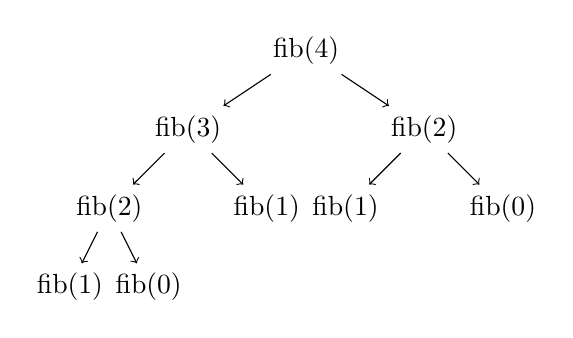
\begin{tikzpicture}
        % nodes
        \node (n1)     at (2.5, 2) {fib(4)};
        \node (n1-1)   at (1, 1) {fib(3)};
        \node (n1-1-1) at (0, 0) {fib(2)};
        \node (n1-1-1-1) at (-0.5, -1) {fib(1)};
        \node (n1-1-1-2) at (0.5, -1) {fib(0)};
        \node (n1-1-2) at (2, 0) {fib(1)};
        \node (n1-2)   at (4, 1) {fib(2)};
        \node (n1-2-1) at (3, 0) {fib(1)};
        \node (n1-2-2) at (5, 0) {fib(0)};
        % arrows
        \draw[->] (n1)     -- (n1-1);
        \draw[->] (n1)     -- (n1-2);
        \draw[->] (n1-1)   -- (n1-1-1);
        \draw[->] (n1-1)   -- (n1-1-2);
        \draw[->] (n1-2)   -- (n1-2-1);
        \draw[->] (n1-2)   -- (n1-2-2);
        \draw[->] (n1-1-1) -- (n1-1-1-1);
        \draw[->] (n1-1-1) -- (n1-1-1-2);
        \end{tikzpicture}
        \caption{Growth of the callstack of \texttt{fib(4)}}
        \label{fib_4_callstack}
    \end{minipage}
    \begin{minipage}[b]{.5\linewidth}
        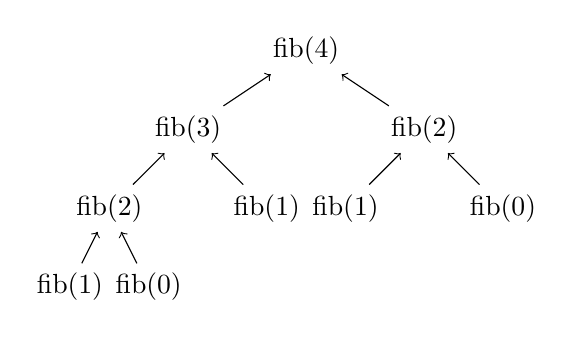
\begin{tikzpicture}
        % nodes
        \node (n1)     at (2.5, 2) {fib(4)};
        \node (n1-1)   at (1, 1) {fib(3)};
        \node (n1-1-1) at (0, 0) {fib(2)};
        \node (n1-1-1-1) at (-0.5, -1) {fib(1)};
        \node (n1-1-1-2) at (0.5, -1) {fib(0)};
        \node (n1-1-2) at (2, 0) {fib(1)};
        \node (n1-2)   at (4, 1) {fib(2)};
        \node (n1-2-1) at (3, 0) {fib(1)};
        \node (n1-2-2) at (5, 0) {fib(0)};
        % arrows
        \draw[<-] (n1)     -- (n1-1);
        \draw[<-] (n1)     -- (n1-2);
        \draw[<-] (n1-1)   -- (n1-1-1);
        \draw[<-] (n1-1)   -- (n1-1-2);
        \draw[<-] (n1-2)   -- (n1-2-1);
        \draw[<-] (n1-2)   -- (n1-2-2);
        \draw[<-] (n1-1-1) -- (n1-1-1-1);
        \draw[<-] (n1-1-1) -- (n1-1-1-2);
        \end{tikzpicture}
        \caption{Evaluation of the callstack of \texttt{fib(4)}}
        \label{fib_4_callstack_evaluation}
    \end{minipage}
\end{figure}

By collecting all calls in a table it is also trivial to remove duplicate calls from the callstack before evaluation (figure z), which gives us memoization which speeds up the translation significantly. The callstack table is just a relational representation of the callstack with memoization (Table T).


Translation begins with a static analysis that compiles the \CASE-expression into standalone predicates and queries (\autoref{fib_analysis_output}). Note how the predicates include the negation of the leading predicates. Beside cutting the UDF into slices the analysis also enumerates the callsites contained in the given scenario. For each callsite the arguments are extracted as standalone queries with only the UDF arguments as free variables. This data is used to do the macro expansion that generate the translated UDF. Chapter \autoref{approach} explains the ins and outs of the inference rules of the static analysis, but in this introduction I continue with the templates and how they work.



\begin{figure}
    \begin{minipage}[b]{.5\linewidth}
    \centering
        \begin{align*}                                    \\
         &\langle~&\text{pred}: ~&\mintinline{postgresql}{SELECT ($1 = 0)}                  ,\\
         &        &\text{query}:~&\mintinline{postgresql}{SELECT 0}                         \rangle\\
        \end{align*}
    \subcaption{Nonrecursive scenarios}\label{fib_nonrec_scenarios}
    \end{minipage}%
    \begin{minipage}[b]{.5\linewidth}
    \centering
        \begin{align*}
        &\big\langle~&\text{pred}:~ &\mintinline{postgresql}{SELECT (NOT $1 = 0) AND ($1 = 1)}  ,\\
        &            &\text{query}:~&\mintinline{postgresql}{SELECT 1 + fib(0)},     \\
        &            &\text{callsites}:~&\langle \text{id}: 1,~\text{args}: (\mintinline{postgresql}{SELECT 0})\rangle\big\rangle,\\
        &\big\langle&\text{pred}:~ &\mintinline{postgresql}{SELECT (NOT $1 = 0) AND (NOT $1 = 1)}  ,\\
        &           &\text{query}:~&\mintinline{postgresql}{SELECT fib($1 - 1) + fib($1 - 2)},     \\
        &           &\text{callsites}:~&\langle \text{id}: 2,~\text{args}: (\mintinline{postgresql}{SELECT $1 - 1})\rangle, \\
        &           &                  &\langle \text{id}: 3,~\text{args}: (\mintinline{postgresql}{SELECT $1 - 2})\rangle\big\rangle\\
        \end{align*}
    \subcaption{Recursive scenarios}\label{fib_rec_scenarios}
    \end{minipage}
    \caption{Output of scenario analysis of \mintinline{postgresql}{fib(int)} from \autoref{intro_fib}}\label{fib_analysis_output}
\end{figure}

        
\begin{figure}
    \centering
            \bgroup
            \def\arraystretch{1.5}
        \begin{tabular}{|c|}\hline
            %\footnotesize\mintinline{postgresql}{in_args := $1 / SELECT c.call_args FROM callstack c}\\
            \begin{tabular}{|l|}\hline
                \footnotesize{Scenario 1}\\
                \begin{tabular}{|l|}\hline
                    \footnotesize{Callsite 1}\\
                    \footnotesize\mintinline{postgresql}{SELECT in_args, callsite.id, callsite.args AS call_args}\\[-5pt]
                    \footnotesize\mintinline{postgresql}{  FROM scenario.pred p WHERE p.v}\\
                \hline \end{tabular}\\
                \mintinline{postgresql}{UNION}\\
                \begin{tabular}{|l|}\hline
                    \footnotesize{Callsite 2}\\
                    \footnotesize\mintinline{postgresql}{SELECT in_args, callsite.id, callsite.args AS call_args}\\[-5pt]
                    \footnotesize\mintinline{postgresql}{  FROM scenario.pred p WHERE p.v}\\
                \hline \end{tabular}\\[2mm]
            \hline \end{tabular}\\
                \mintinline{postgresql}{UNION}\\
            \begin{tabular}{|l|}\hline
                \footnotesize{Scenario 2}\\
                \begin{tabular}{|l|}\hline
                    \footnotesize{Callsite 3}\\
                    \footnotesize\mintinline{postgresql}{SELECT in_args, callsite.id, callsite.args AS call_args}\\[-5pt]
                    \footnotesize\mintinline{postgresql}{  FROM scenario.pred p WHERE p.v}\\
                \hline \end{tabular}\\[2mm]
            \hline \end{tabular}
            \\[6mm]
        \hline
        \end{tabular}
        \egroup
    \caption{Structure of the callstack CTE. In the beginning, the original parameters \$1 are used. The recursive step iterates over all newly discovered calls.}
    \label{discovery_strucutre}
\end{figure}



\begin{figure}
        \newsavebox{\discoveryA}
        \sbox{\discoveryA}{
            \bgroup
            \def\arraystretch{1.5}
            \begin{tabular}{|c|}\hline
                \texttt{in\_args := \$1}\\
                \begin{tabular}{|l|}\hline
                    \footnotesize{Scenario 1}\\
                    \begin{tabular}{|l|}\hline
                        \footnotesize{Callsite 1}\\
                    \hline \end{tabular}\\
                    \begin{tabular}{|l|}\hline
                        \footnotesize{Callsite 2}\\
                    \hline \end{tabular}\\[2mm]
                \hline \end{tabular}\\
                \begin{tabular}{|l|}\hline
                    \footnotesize{Scenario 2}\\
                    \begin{tabular}{|l|}\hline
                        \footnotesize{Callsite 3}\\
                    \hline \end{tabular}\\[2mm]
                \hline \end{tabular}
                \\[6mm]
            \hline
            \end{tabular}
            \egroup
          }
        
        \newsavebox{\discoveryB}
        \sbox{\discoveryB}{
            \bgroup
            \def\arraystretch{1.5}
            \begin{tabular}{|c|}\hline
                \texttt{in\_args := }$\{\ast, \ast \ast\}$\\
                \begin{tabular}{|l|}\hline
                    \footnotesize{Scenario 1}\\
                    \begin{tabular}{|l|}\hline
                        \footnotesize{Callsite 1}\\
                    \hline \end{tabular}\\
                    \begin{tabular}{|l|}\hline
                        \footnotesize{Callsite 2}\\
                    \hline \end{tabular}\\[2mm]
                \hline \end{tabular}\\
                \begin{tabular}{|l|}\hline
                    \footnotesize{Scenario 2}\\
                    \begin{tabular}{|l|}\hline
                        \footnotesize{Callsite 3}\\
                    \hline \end{tabular}\\[2mm]
                \hline \end{tabular}
                \\[6mm]
            \hline
            \end{tabular}
            \egroup
          }
          
        \newsavebox{\discoveryRes}
        \sbox{\discoveryRes}{
        \begin{tabular}{c|c|c}
        \texttt{in\_arg\_1} & \texttt{callsite} & \texttt{call\_arg\_1} \\
        \hline
        \hline
        \texttt{\textcolor{red}{4}} & \texttt{1} & \texttt{3}$\ast\phantom{\ast}$ \\
        \texttt{\textcolor{red}{4}} & \texttt{2} & \texttt{2}$\ast\ast$\\
        \hline
        \end{tabular}
        }
        \begin{tikzpicture}
        \node (discoveryBase) at (0,4) {\usebox{\discoveryA}};\\
        \node (discoveryRec) at (5,4) {\usebox{\discoveryB}};\\
        \node (res) at (2.5, 0) {\usebox{\discoveryRes}};\\
        \draw[->, bend left=10] (discoveryBase) edge (res);
        \draw[->, bend left=10] (res) edge (discoveryRec);
        \draw[->, bend left=10] (discoveryRec) edge (res);
        \end{tikzpicture}
    \caption{Caption}
    \label{callstack_recurse}
\end{figure}

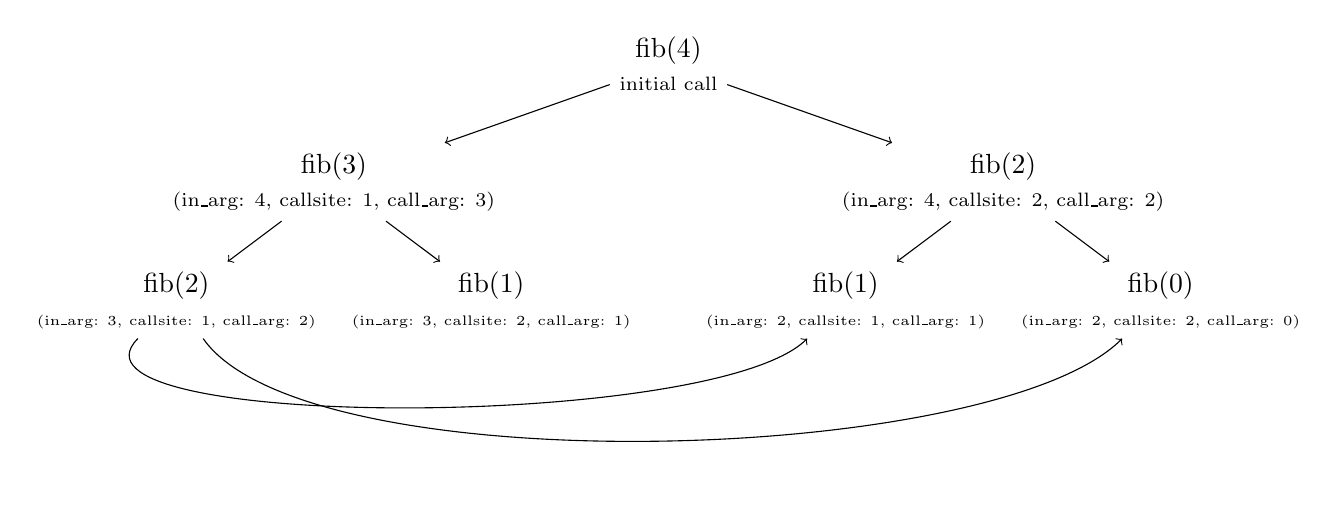
\begin{tikzpicture}[->, level distance=15mm, align=center]
\tikzstyle{level 1}=[sibling distance=85mm]
\tikzstyle{level 2}=[sibling distance=40mm]
\tikzstyle{level 3}=[sibling distance=40mm]
\node{fib(4)\\\scriptsize{initial call}}
  child { node {fib(3)\\\scriptsize{(in\_arg: 4, callsite: 1, call\_arg: 3)}}
    child {node (fib2) {fib(2)\\\tiny{(in\_arg: 3, callsite: 1, call\_arg: 2)}}
      %child {node {fib(1)\\\tiny{(in\_arg: 4, callsite: 2, call\_arg: 2)}} }
      %child {node {fib(0)\\\tiny{(in\_arg: 4, callsite: 2, call\_arg: 2)}} }
    }
    child {node (fib1) {fib(1)\\\tiny{(in\_arg: 3, callsite: 2, call\_arg: 1)}} }
  }
  child {node {fib(2)\\\scriptsize{(in\_arg: 4, callsite: 2, call\_arg: 2)}}
    child {node (fib1) {fib(1)\\\tiny{(in\_arg: 2, callsite: 1, call\_arg: 1)}} }
    child {node (fib0) {fib(0)\\\tiny{(in\_arg: 2, callsite: 2, call\_arg: 0)}} }
  };
\draw[->, bend left=10, out=225, in=225, looseness=0.5] (fib2) edge (fib1);
\draw[->, bend right=5, out=305, in=225, looseness=0.5] (fib2) edge (fib0);
\end{tikzpicture}

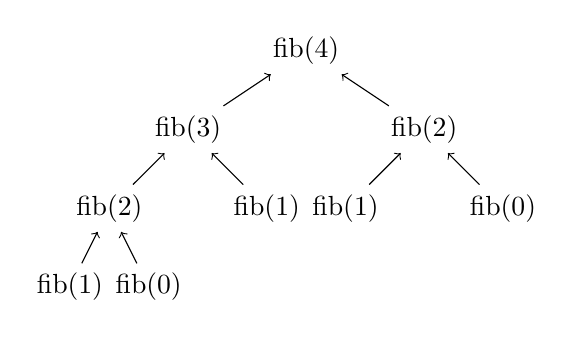
\begin{tikzpicture}
% nodes
\node (n1)     at (2.5, 2) {fib(4)};
\node (n1-1)   at (1, 1) {fib(3)};
\node (n1-1-1) at (0, 0) {fib(2)};
\node (n1-1-1-1) at (-0.5, -1) {fib(1)};
\node (n1-1-1-2) at (0.5, -1) {fib(0)};
\node (n1-1-2) at (2, 0) {fib(1)};
\node (n1-2)   at (4, 1) {fib(2)};
\node (n1-2-1) at (3, 0) {fib(1)};
\node (n1-2-2) at (5, 0) {fib(0)};
% arrows
\draw[<-] (n1)     -- (n1-1);
\draw[<-] (n1)     -- (n1-2);
\draw[<-] (n1-1)   -- (n1-1-1);
\draw[<-] (n1-1)   -- (n1-1-2);
\draw[<-] (n1-2)   -- (n1-2-1);
\draw[<-] (n1-2)   -- (n1-2-2);
\draw[<-] (n1-1-1) -- (n1-1-1-1);
\draw[<-] (n1-1-1) -- (n1-1-1-2);
\end{tikzpicture}

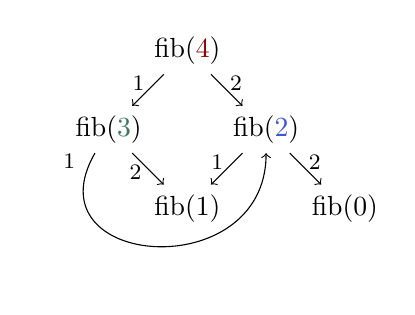
\begin{tikzpicture}[node distance=2cm]
% nodes
\node (f4) at (2, 2) {fib(\textcolor{red}{4})};
\node (f3) at (1, 1) {fib(\textcolor{green}{3})};
\node (f2) at (3, 1) {fib(\textcolor{blue}{2})};
\node (f1) at (2, 0) {fib(1)};
\node (f0) at (4, 0) {fib(0)};
% arrows
\draw[->] (f4) -- (f3) node[pos=0.3,left]{\footnotesize{1}};
\draw[->] (f4) -- (f2) node[pos=0.3,right]{\footnotesize{2}};
\draw[->, out=240, in=270, looseness=2] (f3) edge (f2);
\node (lbl) at (0.5, 0.6) {\footnotesize{1}};
\draw[->] (f3) -- (f1) node[pos=0.6,left]{\footnotesize{2}};
\draw[->] (f2) -- (f1) node[pos=0.3,left]{\footnotesize{1}};
\draw[->]  (f2) -- (f0) node[pos=0.3,right]{\footnotesize{2}};
\end{tikzpicture}

\begin{tabular}{c|c|c}
\texttt{in\_1} & \texttt{callsite} & \texttt{arg\_1} \\
\hline
\hline
\textcolor{red}{4} & 1 & \textcolor{green}{3} \\
\textcolor{red}{4} & 2 & \textcolor{blue}{2} \\
\hline
\textcolor{green}{3} & 1 & 2 \\
\textcolor{green}{3} & 2 & 1 \\
\hline
\textcolor{blue}{2} & 1 & 1 \\
\textcolor{blue}{2} & 2 & 0 \\ 
\end{tabular}


How does the translation work? The first step, the scenario analysis, extracts all possible execution scenarios of a given function. For the Fibonacci UDF given above, the output of the inference rules is the following:\\

As we can see, the \CASE-expression is deconstructed. Note that the predicates resemble exactly the program flow of the \CASE-expression: A \THEN-branch is only evaluated if all leading \WHEN-expressions evaluated to false and the current predicate evaluates to true. The predicate of the \ELSE-branch is just the negation of all previous predicates.



Based on the recursive scenarios, all callsites are enumerated and their arguments extracted to self-contained queries. The recursive cases are enriched with a list of callsites they contain to check later on whether a result for all callsites of an recursive scenario is present yet.
  Callsite 1: (Argument 1: SELECT \$1 - 1) 
  Callsite 2: (Argument 1: SELECT \$1 - 2)
  
Now we have all the data required to construct a query that assembles the callgraph. This is achieved by recursivly collecting the arguments of the callsites of those scenarios that occur under the given input argeters. In the beginning, the original input argeters of the function are used. As we recurse, we iterate through the newly added callsite arguments to collect data of further calls. We end up by a relational encoding of a callgraph.

\sqlcode{snippets/fib_discovery.sql}

, tracking calls down to the basecases (ie. the nonrecursive scenarios) without evaluating anything from the original function except the callsite-arguments. After the creation of the callgraph, we know the input argeters for the basecases and can evaluate them. With the results of the basecases at hand, it is now possible to continue evaluation up the callgraph. For each recursive scenario we check if for all contained callsites with the given input arguments, a result already exists. If so, the call in the recursive scenario is replaced with the reference to the result and the recursive scenario can be evaluated.

% What are the key components of my approach and results? Also include any specific limitations. 
The translation of an UDF is split in two major parts, static analysis and template expansion. During static analysis the original UDF is split into different evaluation scenarios with a predicate under that this scenario will be evaluated. The analysis result is used to choose and fill appropriate templates to build the translated function.

\paragraph*{Static analysis}
%Case analysis: 
%Callsite extraction
%Recursion type detection
%Constant argeter detection
%Hashability checks
This thesis goal is to extend to range of algorithms for which it is easy to write a fairly performing implementation in standard SQL. I provide inference rules to perform a syntax directed analysis of a given SQL UDF that extracts evaluation scenarios alongside with conditions under which each scenario is executed. To analyze the query correclty, it is necessary to track direct and indirect references to callsites while analyzing the query. Callsites are tracked through FROM, subqueries and CTEs and also takes shadowing into account. Extracted scenarios also contain only actually referenced CTEs, deleting unused CTEs that were referenced by other WHEN-branches. The extracted predicates do not contain any callsites so that they can be used to guard the execution of the scenarios. Predicates, Scenarios and Callsite arguments are extracted in a closed form, so that they contain no free variables and can be evaluated independenty from each other. To achieve this, none of these may reference a row-variables from an outside FROM, only table-variables may be referenced, including outside CTEs. This also limits the ability of the UDF to perform meaningful computations that return tabular results, which we forbid entirely for now.

Each scenario is generated from the different branches of a \CASE-statement and the predicates that need to be fulfilled to reach a given \WHEN-branch. Each resulting scenario is semantically equivalent to the original query if its predicate is fulfilled. All scenarios combined are semantically equivalent to the original query. The scenarios are divided into basecases, that do not contain any recursive callsites, and recursive cases that do contain one or more callsites. Some more analysis is performed on the generated scenarios to detect properties of the function like tail recursion.



\paragraph*{Template-based translation}
%Callstack
%Basecases
%TerminationCheck
%Evaluation
From the extracted data an appropriate template is filled, forming the translation. The translation utilizes the iterative nature of WITH RECURSIVE to implement an actual iterative version of the recursive UDF. First, the callstack is discovered by iterativly collecting the new arguments of the callsites in the appropiate scenario. Second, the basecases are evaluated and all new computable results are collected. This repeats until the final result is computed. Cases where the translation would terminate but the original does not are detected and an infinite loop is created to mimic the original behaviour.

The translation template consists of a discovery-phase and an evaluation-phase. During discovery the callstack is built, collecting all recursive calls down to the nonrecursive basecases. From the discovery-table it is now possible to look up the input arguments that lead to a nonrecursive scenario which can be used to begin the recursive evaluation process. As soon as results for all callsites of a given scenario exist, this scenario can be evaluated. The query continues recursively until the argeter of the original call is found in the evaluation table.
    

\paragraph*{Results}
Static analysis is flexible, limitations sound hard, but are not so bad. Generalization to other conditionals is easy possible, implementation is well structured in phases and easy expandable.

The translation is many magnitudes faster than the original naive recursive function. The original fib-function can be called with max fib(23), while the translation handles still fib(100) within ca. 300ms on the same machine. Problem specific optimized solutions still always wins.

\paragraph*{Thesis overview}
First I will establish the backgrounds required for this thesis. The evaluation of SQL-queries, which is important to understand query performance, is covered first. Special focus is laid on the evaluation of WITH RECURSIVE which we utilize to create a translation from a recursive to an actually iterative function. The evaluation of SQL-UDFs is covered then, showing differences in evaluation that lead to the poor performance of recursive UDFs. Important forms of recursion, as well as pros and cons are dicussed afterwards. The background-chapter closes with a short primer on Small step Operational Semantics.

Before I present the rules in depth, I first introduce a couple of preliminaries are necessary to introduce simplyfying notations ans specify constraints on the functions that can be translated.
...
\newpage

%%
\chapter{Background}\label{Introduction}

\section{Relational Databases}\label{theory}

In this chapter I give a short overview about aspects from the area of (relational) database systems that are relevant to my thesis. I introduce the relational data model and its Structured Query Language (SQL). All explanations target PostgreSQL 10.6 as state-of-the-art Database Management System (DBMS).

PostgreSQL 10.6 is used throughout this thesis as RDBMS and SQL-dialect. Its first version was developed as "POSTGRES" at Berkely 1986 \cite[xxxvi ff.]{psql}. It had its first open source release under the name "Postgres95" in 1995 where the own query language PostQUEL was replaced by SQL. As of 1997 and version 6.0 the software is named "PostgreSQL" to reflect its SQL-capabilities \cite[xxxvi ff.]{psql}.

PostgreSQL claims to be "the most advanced open-source database available anywhere" \cite[xxxvii]{psql}. It conforms to most parts of Core SQL:2011 \cite[S. 2198]{psql} and offers great extensibility and introspection. User defined functions, types, operators, index methods, statistics for the planner, procedural languages, foreign data wrappers and rewrite rules are possible. 

\subsection{Relational Data Model}
An integral part of many applications is to retrieve, modify and persist data. Depending on the complexity of the data (eg. plain key-value, hierarchical structured, associations to other data, etc.) and the requirements to the storage system (performance, query capabilities, robustness, multi-user capability, etc.) a number of solutions are viable. Relational Database Management Systems (RDBMS) are a very popular and advanced solution to manage vast amounts of interconnected data efficiently.

The original relational data model dates back to 1970 where E. F. Codd proposes a representation of data in set-theoretic \textit{relations} \cite{codd}. A relation is similar to \textit{table} with named and typed \textit{columns}. An instance of a relation is a set of tuples from the \textit{domain} of each of the columns. A subset of columns in a relation may form a unique \textit{primary key} for each of its tuples that can be included in other tables as \textit{foreign key} to establish references. A relational data model should be normalized to remove redundancies and enforce atomacity.

An important innovation by the relational model was the claim that access of the stored data should be separated from its internal (physical) representation and should be able to change without affecting the logical representation that is used by a program (\textit{data independence}). Instead of manually accessing the physical stored data, the programmer should just use a "data base sublanguage" (Codd) to specify tasks on the logical level, and the DBMS finds automatically an efficient way to perform the task on a physical level \cite[p. 3 ff.]{FoD}.

Based on Codds proposal of a "universal data sublanguage" to define and manipulate a relational model, Chamberlin and Boyce designed a "Structured English Query Language" (SEQUEL) \cite{sequel, sequel2}. The name alone highlights its declarative nature: Say \textit{what} you want, just in simple English. SEQUEL was later renamed to SQL and first standardized in 1987 as SQL:86 (ISO 9075:1987), the latest version to date is SQL:2016 (ISO/IEC 9075:2016). For this thesis, only a subset of the \textit{Data Manipulation Language} (DML) is of interest, namely reading queries.

\subsection{SQL and query evaluation}

Due to their declarative nature, SQL-Queries are no executable programs by themselves. To create an program from the query (a \textit{plan}), it is first parsed into an \textit{Abstract Syntax Tree} (AST, \autoref{fig:fib_ast}). An AST encodes the syntactic structure of the query into the structure of the AST, preserving its semantics. Parsing text into an AST is a standard step in compilation because ASTs are much more suitable to work with \cite[p. 5]{dragenbook}.

\begin{figure}[h!]
    \centering\footnotesize
    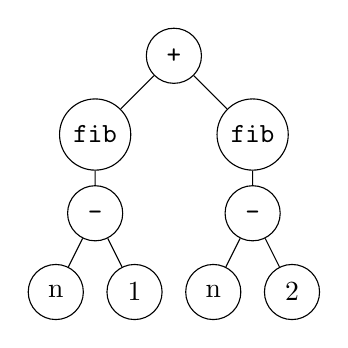
\begin{tikzpicture}[level distance=1cm,level 1/.style={sibling distance=2cm},level 2/.style={sibling distance=1cm}, every node/.style = {shape=circle, draw, align=center, minimum width=7mm, minimum height=7mm}]]
    \node {\texttt{+}}
        child { node{\texttt{fib}}
            child { node {\texttt{-}}
                child { node {n} }
                child { node {1} }
            }
        }
        child { node{\texttt{fib}}
            child { node {\texttt{-}}
                child { node {n} }
                child { node {2} }
            }
        };
    \end{tikzpicture}
    \caption{AST of \texttt{fib(n-1) + fib(n-2)}}
    \label{fig:fib_ast}
\end{figure}

The \textit{parse-tree} of the input query is transformed into a \textit{query-tree}. The transformation to the query-tree includes some desugering like expanding \texttt{T.*} to an explicit column-list, adding default \texttt{ELSE NULL} to \texttt{CASE}-statements and expanding row-comparisons \texttt{(1, 2) = (1, 4)} to boolean conjunctions \texttt{1=1 AND 1=4}. This makes it easier for the query planner to analyze the structure of the query and derive an efficient plan. Finally the query is rewritten, which primary replaces references to views by their original queries. \cite{}

The preprocessed and rewritten query is then fed into the \textit{query planner} to compile the declarative query into an procedural program (a \textit{plan-tree}) executable by the \textit{executor}. Its main responsibility is to find the fastest way to access and join the involved tables. Every (nontrivial) plan has table scans at its leafs. There are multiple ways to scan a table depending on the presence of predicates and auxiliary datastructures (\textit{indices}). Consider the query \texttt{SELECT * FROM T WHERE T.v = 5}. Depending on the size of \texttt{T} and the number of occurrences of \texttt{5} in the column \texttt{T.v} it may be most efficient to do a full \textit{sequential scan} of the entire table, filtering out rows not matching the predicate. If the table is large and there are only few rows with \texttt{T.v = 5}, an \textit{index-scan} may be much faster. With few I/O-operations the matching rows can be selectively retrieved, without reading the entire table. Various statistics are maintained to help the planner estimate the cost for each operation and choose the cheapest plan. \cite[p. 1887]{psql}


Tables in the \texttt{FROM}-clause can be combined (\textit{joined}) by different algorithms. Each algorithm has its own preconditions, strengths and weaknesses, so the choice of the appropriate join-strategy is very important. As each join-algorithm expects exactly two input tables, joining multiple tables results in a binary join-tree. The join order can impact the query performance dramatically as it determines the size of the intermediate join-results. Three tables R, S, T can either be joined as $(R \bowtie S) \bowtie T$ or as $R \bowtie (S \bowtie T)$. In general it is beneficial to choose the option that removes most rows from the result early to avoid investing time in joining rows that are eventually removed. The planner tries to attach predicates from the query to the joins to reduce the size of the join result (\textit{predicate push-down}).

Further nodes in the plan are used for sorting, aggregation, combining queries and others. Obviously, there are a lot of possible plans for a single query. To find the best plan, the query planner computes all possible plans and estimates the cost of each solution based on various statistics to select the cheapest. As the search-space for the planner growths exponentially with the number of involved tables, the exhaustive search switches to a heuristic-driven optimization when a threshold is exceeded \cite[p. 2064 ff.]{psql}.


Finally, the \textit{executor} recursively executes each node of the plan just as long as required by the parent node (Volcano Iterator Model) \cite{volcano}. Thus, each operation is not necessarily performed to completion but just as long as required to return the next row. Each plan contains therefore not only an estimate for the \textit{total cost} of the node until completion, but also minimum cost to return the first row (\textit{start up cost}). In the best case, the first returned row is just the single requested row and eg. the entire remaining table scan can be omitted. Yet, some operations need to be run to completion before being able returning the first row, eg. sorting. For these cases, the start up cost equals the actual cost.




% Building the cartesian product between tables is called a \textit{join}. Even for moderate sized tables the result of a couple of joins can be astronomically large, if done naively. Imagine build the cartesian product a table \texttt{S} with 10.000 rows, \texttt{T} with 100 rows and \texttt{R} with 1.000 rows. The resulting table would have $10.000 * 100 * 1.000 = 1.000.000.000$ rows - that escalated quickly!

% They just specify \textit{what} the user wants to achieve without telling \textit{how} (declarativity \cite[p. 21]{ullman}). To understand the "problem statement" of the user, the query is parsed, checked and rewritten before fed into the query-planner.

% It is possible to output the generated parse- and query-trees to the logfiles with configuration parameters \texttt{debug\_print\_\{parse, rewritten\}} set to true. To sanitize and parse the query-tree again, I used the great library \texttt{PgQueryHauler} by Denis Hirn \cite{denis_hirn} and Peter Richter \cite{peter_richter} to parse the logs and pretty print them as SQL again.

% There may be many possible strategies to execute a query and the best solution depends on various details (physical organization, frequencies of values, auxiliary data-structures, etc. pp) that may help to find the most efficient one. The \textit{query planner} is responsible to generate an actual executable, imperative program called a \textit{plan}.

%They specify \textit{what} the user wants to achieve without requiring any information about the exact \textit{how}. A query to count the number of rows with \texttt{t=0} from a table \textit{T} does state this intent directly as \texttt{SELECT COUNT(*) FROM T WHERE t = 0}. There is no loop incrementing a counter nor any information included about the location or retrieval of the contents of \texttt{T}. The desired result is specified at a high abstraction level and the best way to compute this result is obtained automatically. This property is known as \textit{declarativity}.

% To evaluate the query, the "problem statement" (the query) needs to be translated into a concrete "plan". This translation is done by the query planner.

% But even the query planner is not the holy grail and there are queries that perform incredibly bad or are difficult to formulate in a way the query planner can find a efficient plan.

% The most frequent form of reading queries are $\textit{SELECT s_1, s_2, ..., s_n FROM T_1, T_2, ..., T_n WHERE p}$-queries (S-F-W). The cartesian product $\texttt{T_1 \times T_2 \times \dots \times T_n}$ between the tables is built and the resulting rows are filtered by the predicate \texttt{p}. Finally, the output columns in the select-list are evaluated for each row, returning the output table.
\section{Recursion in SQL}

Recursion is a fundamental concept in everyday programming as well in computability-theory. Every recursive function consists of a number of different \textit{evaluation scenarios}. Some of them cause subsequent recursive calls (\textit{recursive scenarios}) and at least one scenario causes no recursive calls at all. Otherwise, the function will never terminate. We will call nonrecursive scenarios \textit{basecases}. The programmer usually uses conditionals to direct which scenario should be evaluated. For this thesis, I assume that conditionals are given in the form of \texttt{CASE}-expressions only, to that a \textit{predicate} is stated explicitly for each scenario. One of the main task of the translation is to collect the scenarios and identify their predicates.

Recursive functions can be implemented in SQL in two ways: As User Defined Function (UDF) or as self-referential Common Table Expression (CTE) in \texttt{WITH RECURSIVE}-queries. UDFs are functions (actually procedures) as we know them: A function with a name, an argument list, a defined return type and a function body. Recursive CTEs are different, as they are no procedures with explicit arguments but self-referential queries of a specific structure.

\subsection{Recursive User Defined Functions}
Recursive functions can be created in PostgreSQL as UDFs. UDFs can be implemented in a wide range of languages but we consider only SQL-UDFs as the pure SQL approach. There is also a number of ways to specify arguments and add modifiers. For my thesis I use just simple positional arguments without any modifiers (eg. \texttt{\$1}).

\begin{figure}[h!]
    \centering
    \begin{minted}{postgresql}
CREATE FUNCTION fac(INT) RETURNS INT AS $$
SELECT CASE WHEN $1 = 1 THEN 1
            ELSE $1 * fac($1 - 1)
       END
$$ LANGUAGE SQL;

SELECT fac(10);
    \end{minted}
    \caption{Calculation of $10!$ using a a recursive UDF \texttt{fac)}.}
    \label{fig:my_label}
\end{figure}

A UDF is mostly a black box for the query planner. They have just a fixed cost assigned as a whole (default 1000 \cite[p. 1435]{psql}) and the body of every call is repeatedly planned before execution.

Under certain circumstances, PostgreSQL can optimize some function calls. Very simple functions can be inlined during planning \cite{psqlWikiUDFinlining}  (see \autoref{fig:inlining}), but this is done only once, so its impact for recursive functions is not a game-changer.


\begin{figure}[h!]
    \centering
    \begin{minted}{postgresql}
CASE WHEN ($1 = 1) THEN 1
     ELSE ($1 * CASE WHEN (($1 - 1) = 1) THEN 1
                     ELSE (($1 - 1) * fac(($1 - 1) - 1))
                END)
END
    \end{minted}
    \caption{The query-body of \texttt{fac} after the planner has inlined the call to \texttt{fac(\$n - 1)}.}
    \label{fig:inlining}
\end{figure}

Identical calls to an function marked as \texttt{IMMUTABLE} can be folded into a constant during planning \cite[p. 995]{psql}. The impact on usual queries may be significant when a call to an expensive function eg. in a where-clause is repeated for every row of a table:\\
\begin{minted}{postgresql}
SELECT * FROM T WHERE T.v IS BETWEEN fac(99) AND fac(100);
\end{minted}
Instead of evaluating \texttt{fac(99)} and \texttt{fac(100)} exactly $|T|$ times, the planner may be able to evaluate those functions once and replace the values in the where-clause with that values. For recursive SQL-UDFs, this happens as well, but isolated for each invocation of a UDF. There is nothing folded into constants across levels of recursion.

\subsection{Recursive Common Table Expressions}

Common Table Expressions (CTEs) are a convenient way to define auxiliary queries once in advance to use them similar to temporary tables in the contained query. CTEs help breaking down a big query down to smaller individual parts. CTEs are only evaluated once, which can improve performance. On the other hand, CTEs are known to be "optimization fences" as the planner does not perform predicate pushdown into CTEs.


\begin{figure}[h!]
    \centering
    \begin{minted}{postgresql}
WITH RECURSIVE T(i, v) AS (
 SELECT 1, 1
   UNION ALL
 SELECT i + 1, v * (i + 1) FROM T WHERE i < 10
)
SELECT v FROM T WHERE i = 10;
    \end{minted}
    \caption{Calculation of $10!$ using a self-referential CTE.}
    \label{fig:my_label}
\end{figure}


CTEs also exist also in a "recursive" variant, which makes SQL queries much more expressive. Actually, since the introduction of recursive CTEs in SQL:1999, queries are turing-complete. Every intuitively computable function can expressed as a SQL-query. PostgreSQL supports this feature since Version 8.4 (2009) \cite[p. 2811]{psql}. Implementations in PostgreSQL for turing-machines and cyclic tag systems exist, demonstrating this property \cite{psqlWikiCTS, psqlWikiTM}.

Yet, recursive functions need to be implemented in a special style using self-referential CTEs inside \texttt{WITH RECURSIVE}-queries. This constraints origin from the fact that they are actually evaluated iterativly. Each self-referential CTE consist of a \texttt{UNION} or \texttt{UNION ALL} that divides the starting query from the "recursive" query. The recursive query contains a reference to the CTE itself. Evaluation happens in a iterative fashion: In each iteration the self-reference points to a \textit{working table} containing the results from the previous iteration. When using the variant with \texttt{UNION}, each iteration returns only (globally) new rows. The rows from each iteration is added to the result of the CTE.

As soon as the working table is empty, evaluation stops. In the case of \texttt{UNION ALL} this happens only when an iteration returns the empty table. Using \texttt{UNION}, it stops when the iteration returns no previously unseen rows. RCTEs resembles therefore a while loop.

The semantics of a self-referential CTE using \texttt{UNION} can be summarized as follows:

$$
q_0 ~\cup ~\underbrace{q_r(q_0)}_{q_1} ~\cup~ \underbrace{q_r(q_1)}_{q_2}~ \cup~\underbrace{q_r(q_2)}_{q_3}~ \cup ~\hdots ~ \cup ~ \underbrace{q_r(q_n)}_{= \emptyset}
$$

For \texttt{UNION ALL} the set semantics need to be replaced with bag semantics to allow duplicates.

Beside the special structure of a RCTE, they come with two important restrictions. First, only a single (direct) self-reference is allowed in the self-referential query. A simple workaround is to use a CTE that "proxies" access, so this limitation is not severe.

More notably is that only the previous iteration can be referenced. This is a strong limitation as this allows only the convenient formulation of linear recursive functions. In linear recursion a single recursive call leads to a single subsequent call. To evaluate a call, only the result of the previous call is therefore required. The usual workaround is to use \texttt{UNION ALL} semantics to allow duplicates and to add the previous result to the new results. The obvious caveat of this solution is that the resulting table becomes large quickly. After $n$ iterations, the results from the first iteration is contained $n$ times, results from second iteration $n-1$ times and so on. The result table grows quadratically. Furthermore, there must be taken care of including a stopping criterion to eventually prevent include the previous rows again and instead return the empty table.

\newpage

%% 
\section{Operational Semantics}\label{SOS}

\newpage

%%
\chapter{Analysis rules}

This chapter gives detailed insights of how a given query is sliced into its scenarios and predicates by presenting inference rules. Before introducing the actual formal rules, I will first give an intuition of how the translation idea for each language construct works, before formalizing it.

I begin with presenting a set of four rules that are required to translate simple \CASE-expressions. The nonrecursive rules \RREC und \RBASE handle the case when the SQL-fragment is directly a recursive call resp. does not contain any call at all. Analyzing \CASE-expressions is the core of the translation process as it is the original source of any scenario. Each \WHEN-\THEN~branch is processed step by step by the \RWHEN-rule and eventually the \ELSE-branch by the \RELSE-rule.

To translate arbitrary expressions and whole queries we need a couple of more rules. Functions may have a number of recursive operands that can be translated independently from each other to create a number of scenarios of the original function. The same schema can be applied to ~\SELECT-~ and \FROM-lists. Finally, the \WHERE-part is simple since it consists only of a single expression.

Finally, we allow the use of CTEs that come with a couple of complexities. Due to CTEs, it is possible that a recursive sql-fragment does not contain a callsite directly but indirect via the referenced CTE. Furthermore, CTEs can reference other CTEs so it is necessary to track CTE-dependencies and maintain a list of recursive CTEs while taking shadowing into account.

Before the templates can be finally filled, callsite-arguments must be extracted callsites enumerated.

\section{Preliminaries}\label{approach}

Before talking about the inference rules, some preliminary notations need to be established. First, the notion of a \textit{callsite} seems at its first glance trivial but becomes more complex when considering references that may contain callsites or again references to other callsite-containing tables. Second, the effect of shadowing must be formally captured. Third, some simplifying notations and placeholders are introduced to shorten the already lenghtly rules.

\subsection{Subset of SQL}
%\begin{verbatim}
%[ WITH with_query [, ...] ]
%SELECT [ ALL | DISTINCT [ ON ( expression [, ...] ) ] ]
%    [ * | expression [ [ AS ] output_name ] [, ...] ]
%    [ FROM from_item [, ...] ]
%    [ WHERE condition ]
%
%where from_item can be one of:
%    table_name [ * ] [ [ AS ] alias [ ( column_alias [, ...] ) ] ]
%    ( select ) [ AS ] alias [ ( column_alias [, ...] ) ]
%    with_query_name [ [ AS ] alias [ ( column_alias [, ...] ) ] ]
%    function_name ( [ argument [, ...] ] ) [ AS ] alias ( column_definition [, ...] )
%    from_item [ NATURAL ] join_type from_item [ ON join_condition | USING ( join_column [, ...] ) ]
%
%and with_query is:
%    with_query_name [ ( column_name [, ...] ) ] AS ( select | values )
%\end{verbatim}

%\setlength{\grammarparsep}{20pt plus 1pt minus 1pt} % increase separation between rules
%\setlength{\grammarindent}{12em} % increase separation between LHS/RHS 

\begin{figure}[H]
    \begin{minted}{postgresql}
    <query>     ::= [ WITH (<query>) AS <tblAlias>[, ...] ]
                      SELECT [ DISTINCT ] <expr>  AS <colAlias>[, ...]
                    [ FROM <tbl>     AS <tblAlias>[, ...] ]
                    [ WHERE <expr> ]
                 |  <query> <qfun> <query>
    <tbl>       ::= <tblRef> | (<query>) | <fun>([<expr>, ...])
    <expr>      ::=  <const> |  <colRef> |  <fun>([<expr>, ...])
                 |  CASE [WHEN <expr> THEN <expr>, ...] ELSE <expr> END
                 |  ( <query> )
    <fun>       ::= UDFs and sql built-in operators, functions, aggregates that are stable
    <qfun>      ::= UNION [ALL]
    <const>     ::= sql built-in constants
    <tblAlias>  ::= alias(colAlias[, ...])
    <colAlias>  ::= alias
    \end{minted}
    \caption{The subset of SQL we consider throughout this thesis.}
    \label{lst:sql_grammar}
\end{figure}


%\subsection{No VOLATILE functions}
%Without referential transparancy we cannot assume that two function calls within the same query return the same value, making it impossible to use memoization. Therefore, only UDFs markes as STABLE or IMMUTEABLE (38.7. Function Volatility Categories) are translateable.
%Since we use \texttt{UNION} during the evaluation-phase, the rows are checked on equality. This confronts us with a quirk of PostgreSQL: Composite types have no built in function to check equality, thus \texttt{UNION} fails while checking if two composite-types are equal. Later on we will lift this constraint by casting the nonhashable types to and from text.

%Normal UNION require sortable or hashable, but in WITH RECURSIVE it is always hashable, see\footnote{https://www.postgresql-archive.org/Hashable-custom-types-td5801576.html, https://www.postgresql.org/docs/10/static/xindex.html#XINDEX-OPCLASS-DEPENDENCIES, }

\subsection{Notation and vocabulary}
We say a subtree in the query-block of an UDF named $fn$ has or contains a callsite, if and only if the tree contains a node with a call to the function itself or contains a reference to a table that has a callsite. This table in turn does not need to contain an explicit recursive call but can also contain a reference to a table that is recursive by this definition. This comes from the property that table-references are transitive.
\\\\
\subsection{Auxillary notations}
\begin{align*}
    T[a \mapsto \top] &:= T \cup \{a\}\\
    T[a \mapsto \bot] &:= T \setminus \{a\}\\
    T[a_1 \mapsto r_1, ..., a_n \mapsto r_n] &:= T[a_1 \mapsto r_1] \cdots[a_n \mapsto r_n]\\
\end{align*}
\\\\
For the CTE-store $C$ we define an ordered hash-map with the CTE-alias $a$ as key. The empty CTE-store is denoted as $\varnothing$. A new CTE, given by the CTE-body $t$, its predicate $p$ and the set of referenced CTEs on the same level $r$, is specified as $e=(t, p, r)$ alongside with its key $a$. It is appended to $C$ by the following operation: $C[a: e]$. Ordered subsets of $C$ can be retrieved by filtering for matching keys, ignoring keys not found: $C[\{a_1, ..., a_n, a_x\}] = \langle (a_1, t_1, p_1, r_1)_1, \dots, (a_n, t_n, p_n, r_n)_n\rangle$.
\\\\
The auxiliary function $\sigma_{\text{cols}}$ is used to pick columns from the store by name, eg. $\sigma_{a, t, p, r}(C)$ returns the entire store $\langle (a, t, p, r)_1, \dots, (a, t, p, r)_n \rangle$ and $\sigma_p(C) = \langle p_1, \dots, p_n \rangle$ all predicates in the store.
\\\\


% Intuition how scenario analysis works, then formal inference rules are presented
% Begin with four rules to translate the core of each recurisve UDF
% Extending scope to whole queries
% Adding CTEs
% Post processing

% UDF is analyzed and a intermediate representation is created that is used as input for the query template. 
% Each scenario consists of a single path through the case-distinctions of the original query. A predicate is generated alongside to detect when this path is taken. Recursive and nonrecursive scenarios are distinguished.
% Scenarios are generated by recursively applying inference rules to the original function-body. The idea behind each rules is first illustrated before the formal definition is presented
% I will begin with four rules necessary to translate the heart of every recurisve UDF, the CASE-expression. Then I will extend the scope to cover arbitrary "function-alikes" from `+` to whole queries. I complete with rules to handle CTEs, which will introduce a couple of complexities that need special considerations.
% Before the scenarios can be used to fill in the query template, some postprocessing is needed. Callsites need to be enumerated and scenarios must be augmented with a list of contained scenarios. Furthermore, arguments must be extracted to individual queries.

By application of the inference rules we receive a set of nonrecursive scenarios $B$ and a set of recursive scenarios $R$. Each scenario consists of a predicate $p_i$ and the equivalent form of the original query $q_i$ under that predicate.

$$
\Big(
    \overbrace{\big\{
        \underbrace{
            (p_1, q_1)
        }_{\text{scenario 1}}
    \big\}}^{\text{basecase scenarios}}
    ,
    \overbrace{\big\{
        \underbrace{
            (p_2, q_2)
        }_{\text{scenario 2}},
        \underbrace{
            (p_3, q_3)
        }_{\text{scenario 3}}
    \big\}}^{\text{recursive scenarios}}
\Big)
$$

%There are two base-rules that require no more rule application and lead to an immidiate result: \RBASE and \RREC. The \RBASE-rule is applicable when a subtree $q$ contains no recursive calls or references to recursive table-expressions. We directly obtain the resulting tuple $(\{q\}, \emptyset)$. The other case is the \RREC-rule, which handles a subtree $q$ where the root node is the recursive call itself. To comply with the overall restrictions given under X.Y.Z, no argument may have a callsite. If this is given, the rule leads directly to $(\emptyset, \{q\})$. TODO: EXPLAN REF

%All other rules require a callsite somewhere within the query, unwrapping each layer of the query until the callsite is reached or no callsite exists in the subtree. The rules for handling \CASE-statements create for each possible outcome one pruned version while extending the given predicate by the predicate of the taken \WHEN-branch. In contrast to SELECT-statements and CASE-expressions, other parts of the query \textit{can} contain callsites in sibling subtrees. The idea here is to compute all possible outcomes of these subtrees independantly and then build the cartesian-product to receive all possible scenarios of the execution of the parent node. The \REXPR-rule implements purely this idea and the \RCTE and \RFROM-rule come as variations or extensions that take distinct particularities into account.

%The most complicated rule is for handling \WITH-statements. As in the \REXPR-rule, each execution-scenario for every CTE is computed and then the cartesion-product is build over all the scanarios. But two difficulties needs to be considered: First, each CTE can reference previous CTEs from within the same WITH-statement. Second, not every CTE may be referenced later on when the actually query (without the CTEs) is processed - eg. the referencing part may be pruned away after application of a \RWHEN-rule. This leads to to multiple identical versions of the original query that only differ in their predicates, namely by the case-distinctions from the unused CTE. This is semantically not a problem but can degrade performance, since callsites are enumerated based on the set of recursive and nonrecursive cases. Unfortunately, it is hardly possible to postpone this step to postprocessing since we would have to identify and remove the parts caused by the unused CTE from the predicate. Thus we hve two rules for handling CTEs: One for processing and removing each CTE one by one from the query and one for reconstructing the original \WITH-Statement, limited to that CTEs that are actually used by the translated query eventually.

%So, how does the CTE-Rules work in detail? Each CTE is processed on its own, one by one. The processed CTE is removed from the query and put into the variable-store and added alongside with its predicate to the temporary CTE-list. Depending on the processed CTE the recursive or nonrecursive store/list is choosen. Computation continues as long as CTEs are present. Finally, the complete query including CTEs is reconstructed. The actual query is translated with emptied temporary CTE-lists. Only CTEs that are referenced (directly or indirectly) are kept and their predicates are appended to the result predicate. To find out what CTEs are referenced, all free variables under the given environment need to be recursivly followed.

\section{Translating simple case distinctions}
% Goal is to translate a simple CASE-statement
% Start with primitive rules that do not recurse
% Within CASE-expressions the callsite can be located at two different places: WHEN and THEN
% CASE-expressions can be nested, again this can happen in the WHEN and in the THEN part.

For this section, we focus on the set of rules that are involved in every translation. Those rules are the axioms that will eventually add an expression either to $B$ or to $R$. Beside those basic rules, obviously, handling \CASE-distinctions are an integral part of every translation. With those few rules it is already possible to analyze very simple expressions, as we will see in an example.

Notation: Boxes predicates, double-lined box result, Tables scenarios etc.

\subsection{Callsites and basecases}
The inference rules are applied recursively to an initial query, removing each layer one by one. In the end, there are two basecases to that recursion. Either we arrive at a \textit{callsite}, ie. the invocation of the function itself, or the current subtree contains no callsite anymore. In the latter case, it is not necessary to descend any further, we can consider the entire subtree as basecase.

\begin{figure}[h]
    \begin{minipage}[b]{.5\linewidth}
    \centering % BASE
$$\quad(\textsc{base})\inferrule{
   \neg \hasCallsite(T, e) \\
   \neg \text{isElse}(e)
}{
    T, \varnothing \vdash (p, e) \rightarrow (\{(p, e)\},\{\})
}$$
    \subcaption{}\label{rule:base}
    \end{minipage}\hfill
    \begin{minipage}[b]{.5\linewidth}
    \centering % REC
$$\quad(\textsc{rec})\inferrule{
   \forall i \in \{1, ..., n\} : \neg \hasCallsite(T, x_i)
}{
    T, C \vdash (p, fn(x_1, ..., x_n)) \rightarrow (\{\}, \{(p, fn(x_1, ..., x_n))\})
}$$
    \subcaption{Recursive scenarios}\label{rule:rec}
    \end{minipage}
    \caption{Rule (a) assigns any sql-fragment to $B$ if it does not contain any callsites. (b) Does handle callsites by adding them to $R$. Note that the rule enforces the restriction that no callsites may have recursive arguments. For now, please ignore the environment $(T, C)$.}\label{rule:base_and_rec}
\end{figure}

In \autoref{rule:base_and_rec} you can see the axioms \RREC- and \RBASE. They handle the two cases and add either the callsite to the set of recursive cases $R$ or the nonrecursive subtree to $B$.



\subsection{Simple \CASE-expressions}

The other rules that are endeavoured in every nontrivial translation are those for handling \CASE-expressions. They are the original source of any scenario we will generate. As each branch contain a \WHEN-part which establishes a predicate and a \THEN-part that defines the result, there are two places were a callsite can occur and need to be handled appropriately. As \CASE-expressions can be nested, we will take a look at what happens when they are located in the \WHEN-part and in the \THEN-part.

\CASE-expressions in general are a handy way of writing nested \texttt{IF}s. Each \WHEN implies that all preceding \WHEN's have failed, ie. each \WHEN contains an implicit negation of preceding \WHEN's. Our goal is to make this complete, implicit predicate explicit so that it can be executed individually to tell during the callstack discovery phase (\autoref{}) which callsites are reached during each call.

\begin{figure}[h]
    \begin{minipage}[b]{.45\linewidth}
    \centering
    
    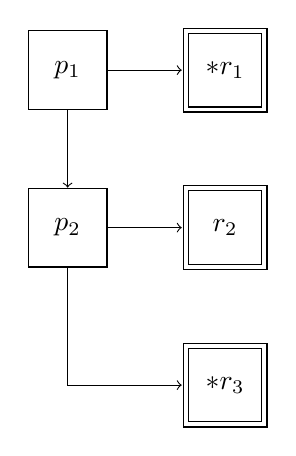
\begin{tikzpicture}[x=20mm, y=20mm]
        \tikzset{Pred/.style={shape=rectangle, draw, minimum width=1cm, minimum height=1cm}}
        \tikzset{Res/.style={shape=rectangle, draw, double distance=0.5mm, outer sep=0.5mm, minimum width=1cm, minimum height=1cm}}
        
        % nodes
        \node[Pred] (p1) at (0, 2) {$p_1$};
        \node[Res]  (r1) at (1, 2) {$\ast r_1$};
        
        \node[Pred] (p2) at (0, 1) {$p_2$};
        \node[Res] (r2) at (1, 1) {$r_2$};
        
        \node[Res] (r3) at (1, 0) {$\ast r_3$};
        
        % arrows
        \draw[->] (p1) -> (r1);
        \draw[->] (p1) -- (p2);
        \draw[->] (p2) -- (r2);
        \draw[->] (p2) |- (r3);
    \end{tikzpicture}
    \subcaption{Logical flow of a simple \CASE-expression with callsites in $r_1$ and $r_3$.}\label{flow:simple_case}
    \end{minipage}\hfill
    \begin{minipage}[b]{.45\linewidth}
    \centering 
    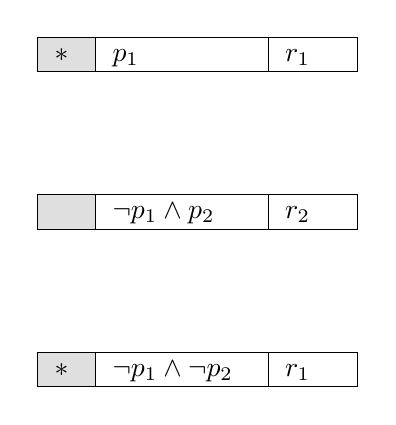
\begin{tikzpicture}[x=20mm, y=20mm]
        \node (case1) at (5, 2) {\begin{tabular}{|p{3mm}|p{5em}|p{2em}|}\hline
        \cellcolor{gray!25} $\ast$ & $p_1$ & $r_1$\\\hline
        \end{tabular}};
        
        \node (case1) at (5, 1) {\begin{tabular}{|p{3mm}|p{5em}|p{2em}|}\hline
        \cellcolor{gray!25} ~~ & $\neg p_1 \land p_2$ & $r_2$\\\hline
        \end{tabular}};
        
        \node (case1) at (5, 0) {\begin{tabular}{|p{3mm}|p{5em}|p{2em}|}\hline
        \cellcolor{gray!25} $\ast$ & $\neg p_1 \land \neg p_2$ & $r_1$\\\hline
        \end{tabular}};
    \end{tikzpicture}
    \subcaption{Recursive scenarios for each branch of the \CASE-expression.}\label{scenarios:simple_case}
    \end{minipage}
    \caption{}\label{rule:base_and_rec}
\end{figure}

%\setlength{\tabcolsep}{2pt}

\autoref{fig:simple_case} visualizes the program flow of a simple \CASE-expression with callsites located in the first \WHEN and in the \ELSE-branch. An arrow to the right means that the predicate is fulfilled, an arrow down denotes the negation. Predicates $p$ are surrounded by a single lined border while doubled bordered box marks a possible result $r$ of the \CASE-statement. An asteriks $\ast$ marks recursive subexpressions. The segmented rectangles at the right show the scenarios generated, an asteriks marks an recursive scenario. The second segment contains the predicate of the scenario, followed by the actual query.

\subsection{Recursive \WHEN's}
Recursive predicates cannot be solved and are therefore considered as part of the result (recursive) expression. Slicing stops before a recursive predicate.

\begin{tikzpicture}[x=20mm, y=20mm]
\tikzset{Pred/.style={shape=rectangle, draw, minimum width=1cm, minimum height=1cm}}
\tikzset{Res/.style={shape=rectangle, draw, double distance=0.5mm, outer sep=0.5mm, minimum width=1cm, minimum height=1cm}}

% nodes
\node[Pred] (p1) at (0, 1.5) {$p_1$};
\node[Res]  (r1) at (1, 1.5) {$r_1$};
\node at (5, 1.5) {\begin{tabular}{|p{3mm}|p{5em}|p{2em}|}\hline
\cellcolor{gray!25} & $p_1$ & $r_1$\\\hline
\end{tabular}};

\node[Res, inner sep=3mm] (res) at (0.5, 0) {
    \begin{tikzpicture}[x=20mm, y=20mm, inner sep=1em]
        \node[Pred] (p2) at (0, 1) {$\ast p_2$};
        \node[Pred] (r2) at (1, 1) {$r_2$};
        \node[Pred] (r3) at (1, 0) {$r_3$};
        \draw[->] (p2) -- (r2);
        \draw[->] (p2) |- (r3);
    \end{tikzpicture}
};
\node at (5, 0) {\begin{tabular}{|c|c|c|}\hline
\cellcolor{gray!25} $\ast$ & $\neg p_1$ & $\WHEN ~p_2~ \THEN ~r_1~ \ELSE ~r_3$\\\hline
\end{tabular}};
% arrows
\draw[->] (p1) -> (r1);
\draw[->] (p1) -> (0, 0.95);
\end{tikzpicture}

\subsection{Nonrecursive subtrees}
Subtrees with no callsite are taken as one big basecase without further slicing.

\begin{tikzpicture}[x=20mm, y=20mm]
\tikzset{Pred/.style={shape=rectangle, draw, minimum width=1cm, minimum height=1cm}}
\tikzset{Res/.style={shape=rectangle, draw, double distance=0.5mm, outer sep=0.5mm, minimum width=1cm, minimum height=1cm}}

% nodes
\node[Pred] (p1) at (0, 1.5) {$p_1$};
\node[Res]  (r1) at (1, 1.5) {$\ast r_1$};
\node at (5, 1.5) {\begin{tabular}{|p{3mm}|p{5em}|p{2em}|}\hline
\cellcolor{gray!25} $\ast$ & $p_1$ & $r_1$\\\hline
\end{tabular}};

\node[Res, inner sep=3mm] (res) at (0.5, 0) {
    \begin{tikzpicture}[x=20mm, y=20mm, inner sep=1em]
        \node[Pred] (p2) at (0, 1) {$p_2$};
        \node[Pred] (r2) at (1, 1) {$r_2$};
        \node[Pred] (r3) at (1, 0) {$r_3$};
        \draw[->] (p2) -- (r2);
        \draw[->] (p2) |- (r3);
    \end{tikzpicture}
};
\node at (5, 0) {\begin{tabular}{|c|c|c|}\hline
\cellcolor{gray!25} ~~ & $\neg p_1$ & $\WHEN ~p_2~ \THEN ~r_1~ \ELSE ~r_3$\\\hline
\end{tabular}};
% arrows
\draw[->] (p1) -> (r1);
\draw[->] (p1) -> (0, 0.95);
\end{tikzpicture}

\subsection{Nested Case in \THEN}
Predicates stack up linearily when nested inside \THEN.


Predicates must be evaluable directly for our translation template, ie. no callsite may be present in any predicate. Therefore, as soon as a predicate appears to be recursive, the recursive predicate is considered part of the recursive result and the evaluation of the \CASE-expression halts with the remaining \CASE-expression which forms an recursive case as a whole.

\begin{tikzpicture}[x=15mm, y=15mm]
\tikzset{Pred/.style={shape=rectangle, draw, minimum width=1cm, minimum height=1cm}}
\tikzset{Box/.style={shape=rectangle, draw, minimum width=1cm, minimum height=1cm, dotted, very thick}}
\tikzset{Res/.style={shape=rectangle, draw, double distance=0.5mm, outer sep=0.5mm, minimum width=1cm, minimum height=1cm}}

% nodes
\node[Pred] (p) at (0, 1) {$p$};
\node[Box]  (r1) at (2, 1) {
    \begin{tikzpicture}[x=15mm, y=15mm]
        \node[Pred] (p1) at (0, 2.5) {$p_1$};
        \node[Res] (r1) at (1, 2.5) {$r_1$};
        
        \node[Pred] (pi) at (0, 1) {$p_i$};
        \node[Res] (ri) at (1, 1) {$r_i$};
        % arrows
        \draw[->] (p1) -- (r1);
        \draw[->] (pi) -- (ri);
        \draw[->, dash pattern=on 5pt off 1pt on 3pt off 3pt on 1pt off 2pt on 1pt off 2pt on 3pt off 1pt] (p1) -- (pi);
        \draw[->, dash pattern=on 5pt off 1pt on 3pt off 3pt on 1pt off 2pt on 1pt off 2pt on 3pt off 1pt] (pi) -- +(0,-1);
    \end{tikzpicture}
};
\node at (5, 2) {
    \begin{tabular}{|p{1em}|p{3cm}|c|}\hline
    \cellcolor{gray!25}  & $p \land \phantom{\neg}p_1 $& $r_1$\\\hline
    \end{tabular}
};
   
\node at (5, 1.4) { 
    \vdots
};
    
\node at (5, 0.65) {
    \begin{tabular}{|p{1em}|p{3cm}|c|}\hline
    \cellcolor{gray!25}  & $p \land \neg p_1 \land \neg p_2 \land \hdots \land p_i$& $r_2$\\\hline
    \end{tabular}
};
% arrows
\draw[->] (p) -- (r1);
\end{tikzpicture}


\iffalse
\begin{tabular}{lllrrrrrrrrrr}
\WHEN ~$p_1$~ \THEN & &                        &         $r_1$&  &$\Rightarrow$ (&     $p_1$ &       &           &         &               &                    &, $r_1$)\\
\WHEN ~$p_2$~ \THEN &(&\WHEN ~$p_{2,1}$~ \THEN &     $r_{2,1}$&  &$\Rightarrow$ (&$\neg p_1$ &$\land$&     $ p_2$& $\land$ &    $ p_{2,1}$ &                    &, $r_{2,1}$)\\
                    & &\WHEN ~$p_{2,2}$~ \THEN &     $r_{2,2}$&  &$\Rightarrow$ (&$\neg p_1$ &$\land$&     $ p_2$& $\land$ &$\neg p_{2,1}$ &                    &, $r_{2,2}$)\\
                    & &\ELSE                   &$\ast r_{2,3}$&) &$\Rightarrow$ (&$\neg p_1$ &$\land$&     $ p_2$& $\land$ &$\neg p_{2,1}$ &$\land \neg p_{2,2}$&, $r_{2,1}$)\\
\ELSE               & &                        &    $\ast r_3$&  &$\Rightarrow$ (&$\neg p_1$ &$\land$& $\neg p_2$&         &               &                    &, $r_3$)\\
\end{tabular}
\fi


\subsection{Nested Case in \WHEN's}
When \CASE-expressions are nested inside \WHEN, there two ways not to receive a given result.

\begin{tikzpicture}[x=15mm, y=15mm]
\tikzset{Pred/.style={shape=rectangle, draw, minimum width=1cm, minimum height=1cm}}
\tikzset{Box/.style={shape=rectangle, draw, minimum width=1cm, minimum height=1cm, dotted, very thick}}
\tikzset{Res/.style={shape=rectangle, draw, double distance=0.5mm, outer sep=0.5mm, minimum width=1cm, minimum height=1cm}}


% nodes
\node[Pred] (p) at (0, 3) {$p$};

\node[Box] (p1) at (0, 1) {
    \begin{tikzpicture}[x=15mm, y=15mm]
        \node[Pred] (p2) at (0, 1) {$\pi_i$};
        \node[Pred] (r2) at (1, 1) {$p_i$};
        % arrows
        \draw[->] (p2) -- (r2);
        \draw[->] (r2) -- +(0, -1);
        \draw[<-, dash pattern=on 5pt off 1pt on 3pt off 3pt on 1pt off 2pt on 1pt off 2pt on 3pt off 1pt] (p2) -- +(0,1);
        \draw[->, dash pattern=on 5pt off 1pt on 3pt off 3pt on 1pt off 2pt on 1pt off 2pt on 3pt off 1pt] (p2) -- +(0,-1);
    \end{tikzpicture}
};
\node[Res] (r1) at (2, 1) {$\ast r_i$};
\node (case1) at (4, 1) {
    \begin{tabular}{|p{1em}|r|c|}\hline
    \cellcolor{gray!25} $\ast$ & $\neg p \land \pi_i \land p_i$ & $r_i$\\\hline
    \end{tabular}
};

\node[Res] (r) at (0, -1) {$\ast r$};
\node (case1) at (4, -1) {
    \begin{tabular}{|p{1em}|rrr|c|}\hline
    \cellcolor{gray!25} $\ast$ & $\neg p \land$ & $     \pi_i$ & $\land \neg p_i$ & $r$\\\hline
    \cellcolor{gray!25} $\ast$ & $\neg p \land$ & $\neg \pi_i$ &                  & $r$\\\hline
    \end{tabular}
};
% arrows
\draw[->] (p) -- (p1);
\draw[->] (p1) -- (r1);
\draw[->] (p1) -- (r);
\end{tikzpicture}

\subsection{\CASE- and \ELSE-rules}

$$\quad(\textsc{when})\inferrule{
    \neg (\hasCallsite(p) \land \hasCallsite(bs))\\
    T, C \vdash (\TRUE, p) \rightarrow (B_p, R_p) \\
    T, C \vdash (\TRUE, e) \rightarrow (B_e, R_e)\\
    B_p = \{(p_{p_1}, p'_1), ..., (p_{p_n}, p'_n)\} \\
    \forall (p_{p_i}, p'_i) \in B_p: T, C \vdash (p_0 ~\AND~ p_{p_i}~\AND~\NOT~ p'_i,~ \CASE bs \END) \rightarrow (B_i, R_i) \\
}{
    T, C \vdash (p_0, \CASE \WHEN p \THEN e ~bs \END) \rightarrow \\\\
    {\begin{tabular}[b]{LLLLLL}
        (&\{&(p_0 ~\AND~ p_p ~\AND~ p' ~\AND~ p_e &, e'&) ~|~~(p_p, p') \in B_p, (p_e, e') \in B_e \} &~\cup~ (\cup_{1\leq i \leq n}B_i), \\
         &\{&(p_0 ~\AND~ p_p ~\AND~ p' ~\AND~ p_e &, e'&) ~|~~(p_p, p') \in B_p, (p_e, e') \in R_e \}&~\cup~ (\cup_{1\leq i \leq n}R_i) ~\cup \\
         &\{&(p_0 ~\AND~ p_p ~\AND~ p_0             &, \CASE \WHEN p'_1 \THEN e ~bs \END&) ~|~~(p_p, p') \in R_p \})
    \end{tabular}}
}$$

$$\quad(\textsc{else})\inferrule{
    T, C \vdash (p, e) \rightarrow (B, R) \\
}{
    T, C \vdash (p, \CASE \ELSE e \END) \rightarrow (B, R)
}$$

\section{Handling recursive operands}

\begin{figure}
    \centering
    \footnotesize
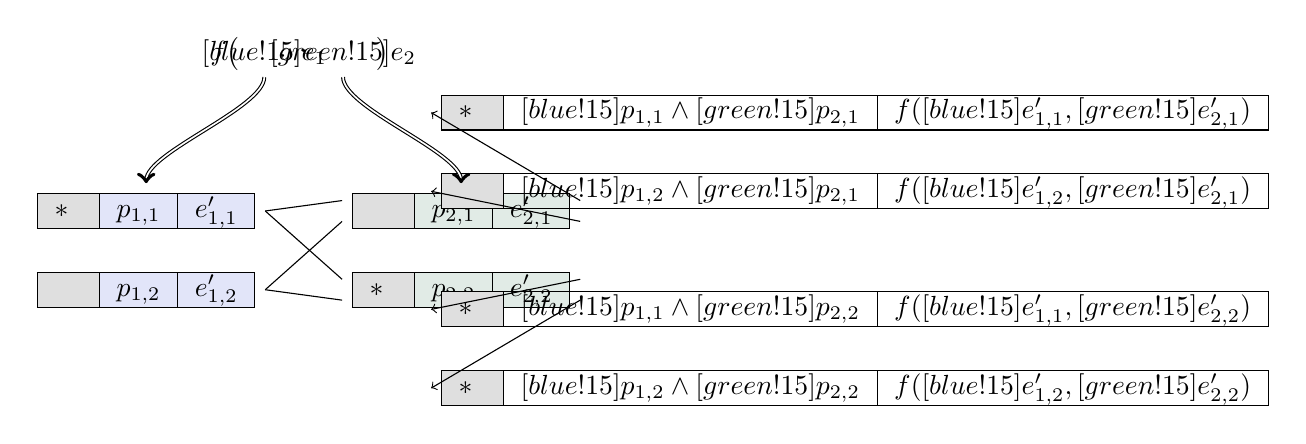
\begin{tikzpicture}[x=10mm, y=10mm]
\node      at (1, 5) {$f\big($};
\node (e1) at (1.5, 5) {$\highlight[blue!15]{e_1}$};
\node      at (2, 5) {$,$};
\node (e2) at (2.5, 5) {$\highlight[green!15]{e_2}$};
\node      at (3, 5) {$\big)$};

\node (e11) at (0, 3) { 
    \begin{tabular}{|p{1em}|r|c|}\hline
    \cellcolor{gray!25} $\ast$ & \cellcolor{blue!15}${p_{1,1}}$ & \cellcolor{blue!15}${e'_{1,1}}$\\\hline
    \end{tabular}
};
\node (e12) at (0, 2) { 
    \begin{tabular}{|p{1em}|r|c|}\hline
    \cellcolor{gray!25}  & \cellcolor{blue!15}${p_{1,2}}$ & \cellcolor{blue!15}${e'_{1,2}}$\\\hline
    \end{tabular}
};

\node (e21) at (4, 3) { 
    \begin{tabular}{|p{1em}|r|c|}\hline
    \cellcolor{gray!25}  & \cellcolor{green!15}${p_{2,1}}$ & \cellcolor{green!15}${e'_{2,1}}$\\\hline
    \end{tabular}
};
\node (e22) at (4, 2) { 
    \begin{tabular}{|p{1em}|r|c|}\hline
    \cellcolor{gray!25}$\ast$ & \cellcolor{green!15}${p_{2,2}}$ & \cellcolor{green!15}${e'_{2,2}}$\\\hline
    \end{tabular}
};

\node (r1) at (9, 4.25) { 
    \begin{tabular}{|p{1em}|r|c|}\hline
    \cellcolor{gray!25} $\ast$ & $\highlight[blue!15]{p_{1,1}} \land \highlight[green!15]{p_{2,1}}$ & $f(\highlight[blue!15]{e'_{1,1}}, \highlight[green!15]{e'_{2,1}})$\\\hline
    \end{tabular}
};
\node (r2) at (9, 3.25) { 
    \begin{tabular}{|p{1em}|r|c|}\hline
    \cellcolor{gray!25}  & $\highlight[blue!15]{p_{1,2}} \land \highlight[green!15]{p_{2,1}}$ & $f(\highlight[blue!15]{e'_{1,2}}, \highlight[green!15]{e'_{2,1}})$\\\hline
    \end{tabular}
};

\node (r3) at (9, 1.75) { 
    \begin{tabular}{|p{1em}|r|c|}\hline
    \cellcolor{gray!25} $\ast$ & $\highlight[blue!15]{p_{1,1}} \land \highlight[green!15]{p_{2,2}}$ & $f(\highlight[blue!15]{e'_{1,1}}, \highlight[green!15]{e'_{2,2}})$\\\hline
    \end{tabular}
};
\node (r4) at (9, 0.75) { 
    \begin{tabular}{|p{1em}|r|c|}\hline
    \cellcolor{gray!25} $\ast$ & $\highlight[blue!15]{p_{1,2}} \land \highlight[green!15]{p_{2,2}}$ & $f(\highlight[blue!15]{e'_{1,2}}, \highlight[green!15]{e'_{2,2}})$\\\hline
    \end{tabular}
};
\draw[->, double, out=270, in=90, looseness = 0.5] (e1.south) to (e11);
\draw[->, double, out=270, in=90, looseness = 0.5] (e2.south) to (e21);

\draw (e11.east) -- (e21.175);
\draw (e11.east) -- (e22.175);
\draw (e12.east) -- (e21.185);
\draw (e12.east) -- (e22.185);

\draw[->] (e21.5) -- (r1.west);
\draw[->] (e21.355) -- (r2.west);
\draw[->] (e22.5) -- (r3.west);
\draw[->] (e22.355) -- (r4.west);
\end{tikzpicture}

    \caption{Operands of a function are translated separately. For each operand a number of scenarios is generated. All possible scenarios of the original function are created by using the cross product.}
    \label{fig:expr-expr}
\end{figure}

\subsection{Single recursive operand}
\subsection{Multiple recursive operands}
\subsection{EXPR-Rule}
$
\inferrule*[Right=(expr)]{
    \inferrule*[Left=(rec)]{ }{
        {\begin{minipage}[b]{15em}
        \mintinline{postgresql}{(TRUE, fib($1 - 1)) ->}
        \mintinline{postgresql}{({}, {(TRUE, fib($1 - 1))})}
        \end{minipage}}
    }\\
    \inferrule*[Right=(rec)]{ }{
        {\begin{minipage}[b]{15em}
        \mintinline{postgresql}{(TRUE, fib($1 - 2)) ->}
        \mintinline{postgresql}{({}, {(TRUE, fib($1 - 2))})}
        \end{minipage}}
    }
}{
    {\begin{minipage}[b]{25em}
    \mintinline{postgresql}{(TRUE, fib($1 - 1) + fib($1 - 2)) ->}
    \mintinline{postgresql}{({}, {(TRUE AND TRUE AND TRUE, fib($1 - 1) + fib($1 - 2))})}
    \end{minipage}}
}
$

$$\quad(\textsc{expr})\inferrule{
    \exists i \in \{1, ..., n\}: T \vdash \hasCallsite(e_i)\\
    \forall i \in \{1, ..., n\}: T, C \vdash (\TRUE, e_i) \rightarrow (B_i, R_i)
}{
    T, C \vdash (p, \oplus_{1\leq i \leq n} e_i) \rightarrow \\\\
    {\begin{tabular}[b]{LLL}
        (&\{(p ~\AND~ (\AND_{1\leq i \leq n} p_i)), \oplus_{1\leq i \leq n} e_i' &~|~~ ((p_1, e_1'), ..., (p_n, e_n')) \in \times_{\{i|1\leq i \leq n\}} ~B_i\}, \\
        &\{(p ~\AND~ (\AND_{1\leq i \leq n } p_i)), \oplus_{1\leq i \leq n} e_i &~|~~ ((p_1, e_1'), ..., (p_n, e_n')) \in \times_{\{i|1\leq i \leq n\}} (B_i \cup R_i),\\&&~~~~\exists e \in \{e'_1, ..., e'_n\} : \hasCallsite(T, e)\})
    \end{tabular}}
}$$
\\

\begin{figure}
    \centering
    {\small
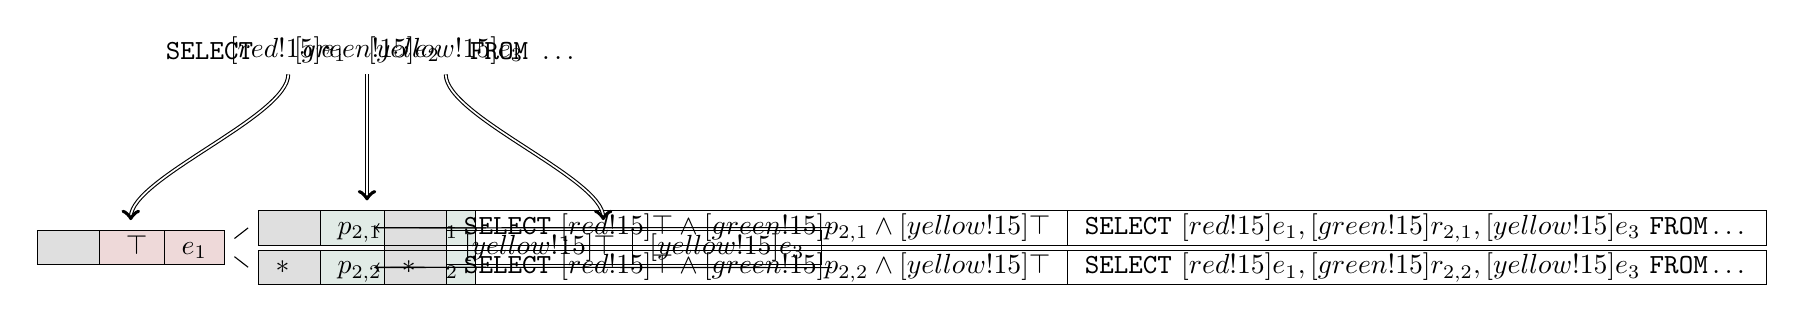
\begin{tikzpicture}[x=5mm, y=5mm]
\node      at ( 8, 9) {$\SELECT$};
\node (e1) at (10, 9) {$\highlight[red!15]{e_1}$};
\node      at (11, 9) {$,$};
\node (e2) at (12, 9) {$\highlight[green!15]{e_2}$};
\node      at (13, 9) {$,$};
\node (e3) at (14, 9) {$\highlight[yellow!15]{e_3}$};
\node      at (16, 9) {$\FROM ~ \dots$};

\node (e11) at (6, 4) { 
    \begin{tabular}{|p{1em}|r|c|}\hline
    \cellcolor{gray!25}  & \cellcolor{red!15} $\top$ & \cellcolor{red!15}$e_1$\\\hline
    \end{tabular}
};

\node (e21) at (12, 4.5) { 
    \begin{tabular}{|p{1em}|r|c|}\hline
    \cellcolor{gray!25}  & \cellcolor{green!15}$p_{2,1}$ & \cellcolor{green!15}$r_{2,1}$\\\hline
    \end{tabular}
};
\node (e22) at (12, 3.5) { 
    \begin{tabular}{|p{1em}|r|c|}\hline
    \cellcolor{gray!25} $\ast$ & \cellcolor{green!15}$p_{2,2}$ & \cellcolor{green!15}$r_{2,2}$\\\hline
    \end{tabular}
};

\node (e31) at (18, 4) { 
    \begin{tabular}{|p{1em}|r|c|}\hline
    \cellcolor{gray!25} & $\highlight[yellow!15]{\top}$ & $\highlight[yellow!15]{e_3}$\\\hline
    \end{tabular}
};

\node (r1) at (30, 4.5) { 
    \begin{tabular}{|p{1em}|r|c|}\hline
    \cellcolor{gray!25}  & $\SELECT ~ \highlight[red!15]{\top} \land \highlight[green!15]{p_{2,1}} \land \highlight[yellow!15]{\top}$ & $\SELECT~ \highlight[red!15]{e_1}, \highlight[green!15]{r_{2,1}}, \highlight[yellow!15]{e_3} ~ \FROM \dots$\\\hline
    \end{tabular}
};
\node (r2) at (30, 3.5) { 
    \begin{tabular}{|p{1em}|r|c|}\hline
    \cellcolor{gray!25} $\ast$ & $\SELECT ~ \highlight[red!15]{\top} \land \highlight[green!15]{p_{2,2}} \land \highlight[yellow!15]{\top}$ & $\SELECT~ \highlight[red!15]{e_1}, \highlight[green!15]{r_{2,2}}, \highlight[yellow!15]{e_3} ~ \FROM \dots$\\\hline
    \end{tabular}
};
\draw[->, double, out=270, in=90, looseness = 0.5] (e1.south) to (e11);
\draw[->, double, out=270, in=90, looseness = 0.5] (e2.south) to (e21);
\draw[->, double, out=270, in=90, looseness = 0.5] (e3.south) to (e31);
\draw (e11.5) to (e21.west);
\draw (e11.355) to (e22.west);
\draw (e21.east) to (e31.175);
\draw (e22.east) to (e31.185);
\draw[->] (e31.5) -- (r1.west);
\draw[->] (e31.355) -- (r2.west);
%\draw[->, bend left=20]  (e11.north) to (e21.north) to (e31.north) to (r1.west);
%\draw[->, bend right=20] (e11.south) to (e22.south) to (e31.south) to (r2.west);
\end{tikzpicture}}
    \caption{The projection of a relation happening inside \SELECT~can be understood as a function $\SELECT(e_1, \dots, e_n, T)$. The same happens analogously for the \FROM-clause: $\FROM(T_1, \dots, T_m)$}
    \label{fig:expr-select}
\end{figure}

\begin{figure}
    \centering
    {\small
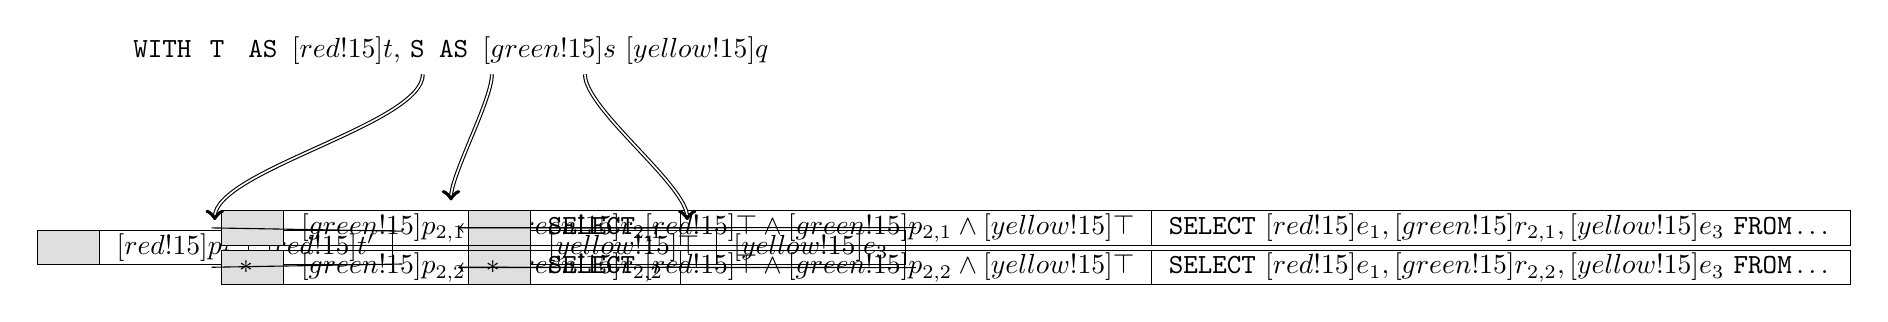
\begin{tikzpicture}[x=5mm, y=5mm, node distance=1mm]
\node (ctes) at (12,9) {\WITH~ \texttt{T} \AS $\highlight[red!15]{t}$, \texttt{S}\AS $\highlight[green!15]{s}$ $\highlight[yellow!15]{q}$};

\node (e11) at (6, 4) { 
    \begin{tabular}{|p{1em}|r|c|}\hline
    \cellcolor{gray!25}  & $\highlight[red!15]{p_t}$ & $\highlight[red!15]{t'}$\\\hline
    \end{tabular}
};

\node (e21) at (12, 4.5) { 
    \begin{tabular}{|p{1em}|r|c|}\hline
    \cellcolor{gray!25}  & $\highlight[green!15]{p_{2,1}}$ & $\highlight[green!15]{r_{2,1}}$\\\hline
    \end{tabular}
};
\node (e22) at (12, 3.5) { 
    \begin{tabular}{|p{1em}|r|c|}\hline
    \cellcolor{gray!25} $\ast$ & $\highlight[green!15]{p_{2,2}}$ & $\highlight[green!15]{r_{2,2}}$\\\hline
    \end{tabular}
};

\node (e31) at (18, 4) { 
    \begin{tabular}{|p{1em}|r|c|}\hline
    \cellcolor{gray!25} & $\highlight[yellow!15]{\top}$ & $\highlight[yellow!15]{e_3}$\\\hline
    \end{tabular}
};

\node (r1) at (30, 4.5) { 
    \begin{tabular}{|p{1em}|r|c|}\hline
    \cellcolor{gray!25}  & $\SELECT ~ \highlight[red!15]{\top} \land \highlight[green!15]{p_{2,1}} \land \highlight[yellow!15]{\top}$ & $\SELECT~ \highlight[red!15]{e_1}, \highlight[green!15]{r_{2,1}}, \highlight[yellow!15]{e_3} ~ \FROM \dots$\\\hline
    \end{tabular}
};
\node (r2) at (30, 3.5) { 
    \begin{tabular}{|p{1em}|r|c|}\hline
    \cellcolor{gray!25} $\ast$ & $\SELECT ~ \highlight[red!15]{\top} \land \highlight[green!15]{p_{2,2}} \land \highlight[yellow!15]{\top}$ & $\SELECT~ \highlight[red!15]{e_1}, \highlight[green!15]{r_{2,2}}, \highlight[yellow!15]{e_3} ~ \FROM \dots$\\\hline
    \end{tabular}
};
\draw[->, double, out=270, in=90, looseness = 0.5] (ctes.220) to (e11);
\draw[->, double, out=270, in=90, looseness = 0.5] (ctes.330) to (e21);
\draw[->, double, out=270, in=90, looseness = 0.5] (ctes.350) to (e31);
\draw (e11.5) to (e21.west);
\draw (e11.355) to (e22.west);
\draw (e21.east) to (e31.175);
\draw (e22.east) to (e31.185);
\draw[->] (e31.5) -- (r1.west);
\draw[->] (e31.355) -- (r2.west);
%\draw[->, bend left=20]  (e11.north) to (e21.north) to (e31.north) to (r1.west);
%\draw[->, bend right=20] (e11.south) to (e22.south) to (e31.south) to (r2.west);
\end{tikzpicture}}
    \caption{The ~\WITH-clause could also be viewed as composition of functions $\WITH(t, T, q)$ that binds a table-variable \texttt{T} to an expression \texttt{t} for a given query \texttt{q}. In this example it would be $\WITH(T, t, \WITH(S, s, q))$ as CTEs can reference preceding ones.}
    \label{fig:expr-cte}
\end{figure}

If the callsites of a query a located in the \FROM-part, it means that at least one table referenced is recursive, ie. contains a callsite or a reference a recursive table. 
As the tables within the same \FROM cannot reference each other, we can process each table independently and resemble the whole query with all possible combinations, similar to the \REXPR-rule. For an example see this example:
\sqlcode[mathescape=true]{snippets/rule_from_example.sql}


$
\inferrule*{
    \inferrule*{...}{
{\begin{minipage}[b]{12em}
\sqlcode{snippets/rules/fib/01-case.sql}
\end{minipage}}
    }
}{
{\begin{minipage}[b]{12em}
\sqlcode{snippets/rules/fib/01-select.sql}
\end{minipage}}
}
$


$$\quad(\textsc{select})\inferrule{
    \exists i \in \{1, ..., k\}: T \vdash \hasCallsite(e_{s_i}) \\
    \forall i \in \{1 \leq i \leq n\} : T \vdash \neg \hasCallsite(e_{t_i}) \\
    T \vdash \neg \hasCallsite(e_{w}) \\
    \forall i \in \{1, ..., k\}: T, \varnothing \vdash (\TRUE, e_{s_i}) \rightarrow (B_i, R_i)
}{
    T, \varnothing \vdash (p, \SELECT [\texttt{DISTINCT}]~ e_{s_1}, ..., e_{s_k} \FROM t_1 \AS a_1 \otimes ... \otimes  t_n \AS a_n \WHERE e_w) \rightarrow \\\\
    {\begin{tabular}[b]{LLLL}
    (~~&\{&(&\SELECT p ~\AND~ p_{s_1} ~\AND~ \cdots ~\AND~ p_{s_k},\\
        &&&\SELECT [\texttt{DISTINCT}]~ e'_{s_1}, ..., e'_{s_k} \FROM t_1 \AS a_1 \otimes ... \otimes  t_n \AS a_n \WHERE e_w~~) \\
        && | &~((p_{s_1}, e'_{s_1}), ..., (p_{s_k}, e'_{s_k})) \in \times_{1 \leq i \leq k} B_i~~\}, \\
     &\{&(&\SELECT p ~\AND~ p_{s_1} ~\AND~ \cdots ~\AND~ p_{s_k}, \\
        &&&\SELECT [\texttt{DISTINCT}]~ e'_{s_1}, ..., e'_{s_k} \FROM t_1 \AS a_1 \otimes ... \otimes  t_n \AS a_n \WHERE e_w~~) \\
        && | &~((p_{s_1}, e'_{s_1}), ..., (p_{s_k}, e'_{s_k})) \in \times_{1 \leq i \leq k} (B_i \cup R_i), \exists e \in \{e'_{s_1}, ..., e'_{s_k}\} : \hasCallsite(e)~~\}~~)\\
    \end{tabular}}
}$$
\subsection{WHERE-Rule}
$$\quad(\textsc{where})\inferrule{
    T \vdash \neg \hasCallsite(e_{s}) \\
    \forall i \in \{1 \leq i \leq n\} : T \vdash \neg \hasCallsite(e_{t_i}) \\
    T \vdash \hasCallsite(e_{w}) \\
    T, \varnothing \vdash (p, e_{w}) \rightarrow (B, R)
}{
    T, \varnothing \vdash (p, \SELECT e_s \FROM t_1 \AS a_1 \otimes ... \otimes  t_n \AS a_n \WHERE e_w) \rightarrow \\\\
    {\begin{tabular}[b]{LLLL}
    (~~&\{&(&\SELECT p_w  \FROM t_1 \AS a_1 \otimes ... \otimes  t_n \AS a_n \WHERE e'_w,\\
        &&&\SELECT e_s \FROM t_1 \AS a_1 \otimes ... \otimes  t_n \AS a_n \WHERE e'_w~~) \\
        && | &~(p_w, e'_w) \in B~~\}, \\
     &\{&(&\SELECT p_w \FROM t_1 \AS a_1 \otimes ... \otimes  t_n \AS a_n \WHERE e'_w, \\
        &&&\SELECT e_s \FROM t_1 \AS a_1 \otimes ... \otimes  t_n \AS a_n \WHERE e'_w~~) \\
        && | &~(p_w, e'_w) \in R~~\}~~)\\
    \end{tabular}}
}$$
\\
\section{Handling CTEs}
% Without CTEs hasCallsite just checks the subtree
The notion of \textit{containing a callsite} (or being \textit{recursive}) is simple when considering only S-F-W queries. If a sql-fragment $e$ contains a callsite, the subexpression is recursive: $\hasCallsite(e) = fn \sqsubset e$. From an implementation point of view, it is as simple as filtering the AST of $e$ for callsites.

(\autoref{fig:trimmed_ref}), (\autoref{fig:simple_indiref})

\begin{wrapfigure}{r}{.5\textwidth}\vspace{-5mm} 
    \begin{minipage}{\linewidth}
    \label{fig:simple_indiref}\par\vfill
    \begin{minted}{sql}
    WITH S AS (SELECT f(n-1)),
         T AS (SELECT * FROM S)
    SELECT * FROM T
    \end{minted}
    \subcaption{Neither the actual query nor the referenced CTE \texttt{T} directly contains a callsite.}
    \label{fib_nonrec_scenarios}\par\vfill
    \begin{minted}{sql}
    SELECT (
        WITH T AS (SELECT f(n-1))
        SELECT 1
    )
    \end{minted}
    \subcaption{Our definition of $\hasCallsite$ would fail here since a callsite is located in the subtree. The query is acutally nonrecursive.}
    \label{fig:trimmed_ref}
\end{minipage}
\caption{}
\label{lst:indirect_callsite_ref}\vspace{-5mm} 
\end{wrapfigure}

% CTEs introduce indirect callsites that make callsite detection more complicated
With CTEs we need to take into account two things. First, callsites can now be located outside the current subtree. Second, the scenario may contain unused recursive CTEs, fooling $\hasCallsite$ stated above to believe a given SQL-fragment is recursive, even if the recursive CTEs are never evaluated.

% Removing all CTEs, translating then and then reattaching only used CTEs fixes this.
We can work around this issues, if we remove the CTEs from the original query before translating the actual query. For each query-scenario only those CTEs are reattached afterwards, that are actually used (\autoref{tracking_recursive_ctes}). To detect indirect callsite references, we note recursive CTEs when detaching (\autoref{tracking_cte_dependencies}) and check against that list if we encounter unbound table-variables.

\subsection{Tracking recursive CTEs}\label{tracking_recursive_ctes}

% Recursive CTEs are gathered step by step 
CTEs are processed individually step by step before the actual query. If a CTE contains a callsite, its alias is added to the list of recursive CTEs in scope $T$. Otherwise, the alias is removed from that list to take shadowing into account as CTEs can be nested (\autoref{lst:indirect_callsite_ref}). As we continue with the following CTEs, any CTE that has no direct callsite but contains a reference to a CTE in $T$, is also added itself to $T$ as the evaluation of that CTE will eventually lead to a recursive call. This way, we can build up $T$ incrementally and do not need to track each reference recursively back to its declaration to find out whether its recursive. For an example see \autoref{fig:tracking_recursive_ctes}

\begin{figure}[h]
    \small
    \centering
    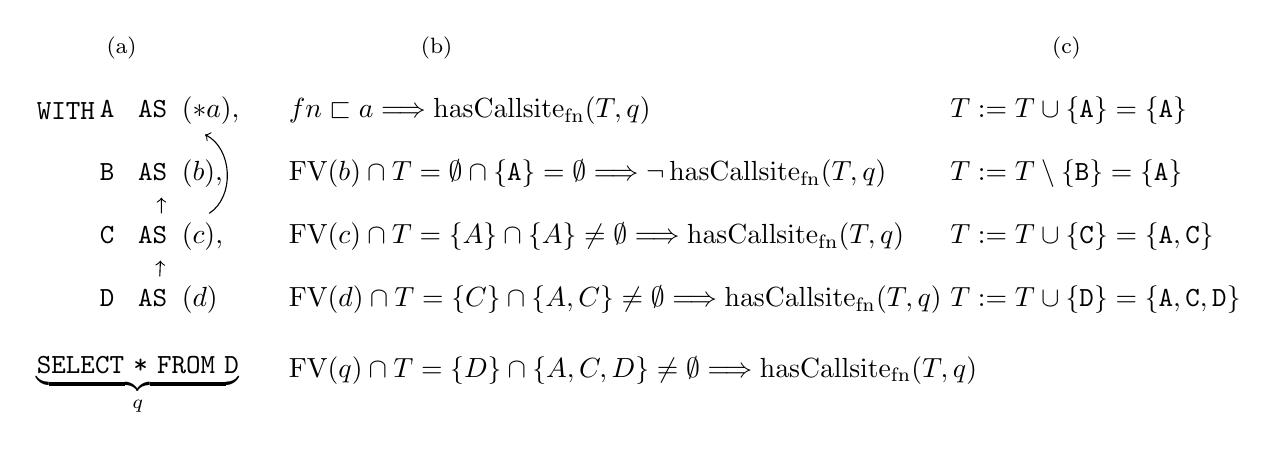
\begin{tikzpicture}[x=8mm, y=8mm]
    \node at (0.5, 1) {\footnotesize{(a)}};
    \node at (5.5, 1) {\footnotesize{(b)}};
    \node at (15.5, 1) {\footnotesize{(c)}};
    \node[anchor=west] at (-1, 0) {\WITH};
    \node[anchor=west] (A) at (0, 0)  {\texttt{A} \AS $(\ast a),$};
    \node[anchor=west] (B) at (0, -1) {\texttt{B} \AS $(b),$};
    \node[anchor=west] (C) at (0, -2) {\texttt{C} \AS $(c),$};
    \node[anchor=west] (D) at (0, -3) {\texttt{D} \AS $(d)$};
    \node[anchor=north west] (S) at (-1, -3.75) {$\underbrace{\SELECT~\texttt{*}~\FROM~\texttt{D}}_q$};
    \node[anchor=west] (Ar) at (3, 0)  {$fn \sqsubset a  \Longrightarrow  \hasCallsite(T, q)$};
    \node[anchor=west] (Br) at (3, -1) {$\FV(b) \cap T = \emptyset \cap \{\texttt{A}\} = \emptyset  \Longrightarrow  \neg \hasCallsite(T, q)$};
    \node[anchor=west] (Cr) at (3, -2) {$\FV(c) \cap T = \{A\} \cap \{A\} \neq \emptyset  \Longrightarrow  \hasCallsite(T, q)$};
    \node[anchor=west] (Dr) at (3, -3) {$\FV(d) \cap T = \{C\} \cap \{A, C\} \neq \emptyset  \Longrightarrow  \hasCallsite(T, q)$};
    \node[anchor=north west] (Dr) at (3, -3.75) {$\FV(q) \cap T = \{D\} \cap \{A, C, D\} \neq \emptyset  \Longrightarrow  \hasCallsite(T, q)$};
    \node[anchor=west] (Ar) at (13.5, 0) {$T := T \cup \{\texttt{A}\} = \{\texttt{A}\}$};
    \node[anchor=west] (Br) at (13.5, -1) {$T := T \setminus \{\texttt{B}\} = \{\texttt{A}\}$};
    \node[anchor=west] (Cr) at (13.5, -2) {$T := T \cup \{\texttt{C}\} = \{\texttt{A}, \texttt{C}\}$};
    \node[anchor=west] (Dr) at (13.5, -3) {$T := T \cup \{\texttt{D}\}= \{\texttt{A}, \texttt{C}, \texttt{D}\}$};
    \draw[->, bend right=60] (C) to (A);
    \draw[->] (C) to (B);
    \draw[->] (D) to (C);
    \end{tikzpicture}
    \caption{a) $q$ has no direct callsite, but reference \texttt{D} that contains a reference to \texttt{A} via \texttt{C}. \texttt{A} contains a direct callsite. b) A fragment $e$ is considered recursive if it contains a direct callsite ($fn \sqsubset$ e) or uses a recursive table-variable. c) If $\hasCallsite$ yields true for a CTE-body, its alias is added to the set of recursive table-variables $T$. Otherwise, the alias is removed to take into account shadowing.}
    \label{fig:tracking_recursive_ctes}
\end{figure}

% Referenced CTEs are detected via unbound variables
References to CTEs can be easily extracted from a sql-fragment by collecting unbound table-variables. Let us call the function that computes all free table-variables of a sql-fragment $e$ $\FV(e)$. It is implemented straight forward: Each CTE definition within a \WITH-block adds its alias to the list of bound table-variables. Every reference to a table-variable that is not contained in that list is considered free.


\begin{wrapfigure}{r}{0.4\textwidth}
    \begin{minted}{sql}
    WITH T AS (SELECT fn(n-1))
    SELECT *
    FROM (
      WITH T AS (SELECT 1)
      SELECT * FROM T
    ) T
    \end{minted}
    \caption{The outer, recursive CTE \texttt{T} is shadowed by an inner CTE.}
    \label{lst:indirect_callsite_ref}
\end{wrapfigure}

% Row-references vs. table-variables
Note that there can occur two different types of free variables inside a sql-fragment: \textit{Table-Variables} and \textit{Row-References}. Table-variables like \texttt{T} can exclusively be used in ~\FROM~ and reference an entire table. This table-variables are introduced either by the existence of a table in the current database or by an CTE. Row-references like \texttt{T.v} point to a single table-row of a table referenced by ~\FROM. Not the actual "use" of a table-variable via a row-reference causes the recursive call, but its bare existence in the FROM-clause since it is evaluated first. For this reason it is sufficient to track only \textit{table}-variables and ignore row-references entirely.

The function to judge whether a sql-fragment is recursive looks now as follows:
\begin{align*}
    \hasCallsite(T, e) =& fn(\dots) \sqsubset e \lor \FV(e) \cap T \neq \emptyset
\end{align*}
Either the callsite is directly contained in $e$, or it has a free table-variable that is also enlisted in $T$. Otherwise the snippet is not recursive.

%We process CTEs of a \WITH-block top down, before translating the actual \SELECT-query, resembling the way SQL evaluates them. If a CTE \texttt{T} references a CTE \texttt{S} that is recursive, \texttt{T} is also recursive. SQL evaluates CTEs in the order they are defined, so that preceding CTEs can be referenced by following CTEs (figure 4.4a FIXME?). Furthermore, CTEs can be nested so that we need to take care of shadowing out outer CTEs.

%Instead of tracing every reference through the entire query until the initial definition is found, I take an incremental approach: If a new table-variable is created, we check each free variable in its subtree against the environment of known recursive table-references within that scope. If there is a recursive table referenced or the subtree contains an immediate recursive call, the new table-reference is entailed the set of recursive table-references.

%Each CTE-scenario is augmented with its dependencies to previously defined CTEs. Each CTE is sliced into its different scenarios, then each scenario is analyzed, removed from the query and stored in the queue. When all CTEs are processed and the actual query is translated, only those CTEs are reattached to the query-scenario that are actually used. Indirect callsites can be detected by simply checking if there exists a free table-variable that is enlisted in $T$.

\subsection{Tracking CTE-dependencies}\label{tracking_cte_dependencies}
As we have seen, CTEs may use other CTEs so that we need to keep track of the CTE dependencies of a query. This happens similar to the creation of the set $T$ of recursive CTEs. For each CTE \texttt{C} we collect all CTE-references \texttt{$C_i$} and add them to the set of dependencies $D_c$. Because the used CTEs may have again dependencies, they are also added to $D_c$. Because of the linear ordering we can do this step by step. See \autoref{fig:cte_deps} for an illustration.

$$\refs(q) := \FV(q) \cup \left(\bigcup_{c \in \FV(q)} \refs(c)\right)$$

\begin{figure}[h]
    \centering
    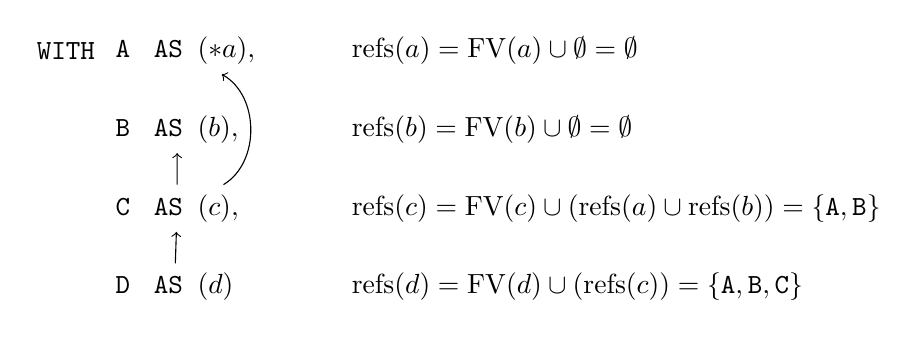
\begin{tikzpicture}[x=10mm, y=10mm]
    \node[anchor=west] at (-1, 0) {\WITH};
    \node[anchor=west] (A) at (0, 0)  {\texttt{A} \AS $(\ast a),$};
    \node[anchor=west] (B) at (0, -1) {\texttt{B} \AS $(b),$};
    \node[anchor=west] (C) at (0, -2) {\texttt{C} \AS $(c),$};
    \node[anchor=west] (D) at (0, -3) {\texttt{D} \AS $(d)$};
    \node[anchor=west] (Ar) at (3, 0)  {$\refs(a) = \FV(a) \cup \emptyset = \emptyset$};
    \node[anchor=west] (Br) at (3, -1) {$\refs(b) = \FV(b) \cup \emptyset = \emptyset$};
    \node[anchor=west] (Cr) at (3, -2) {$\refs(c) = \FV(c) \cup (\refs(a) \cup \refs(b)) = \{\texttt{A}, \texttt{B}\}$};
    \node[anchor=west] (Dr) at (3, -3) {$\refs(d) = \FV(d) \cup (\refs(c)) = \{\texttt{A}, \texttt{B}, \texttt{C}\}$};
    \draw[->, bend right=60] (C) to (A);
    \draw[->] (C) to (B);
    \draw[->] (D) to (C);
    \end{tikzpicture}
    \caption{References are tracked incrementally by collecting free table-variables (ie. direct CTE references) along with the references of those free table-variables.}
    \label{fig:cte_deps}
\end{figure}

While shadowing was an issue when tracking recursive CTEs, it does not hit us here. The difference is that $T$ was passed down while $C$ is only nonempty at the current nesting-level. Any new CTE in a subexpression $e$ binds the previously free table-variable, preventing it from occurring in the CTE-dependencies. Thus, $\FV(e)$ already takes care of shadowing here.

\begin{figure}[h]
    \centering
    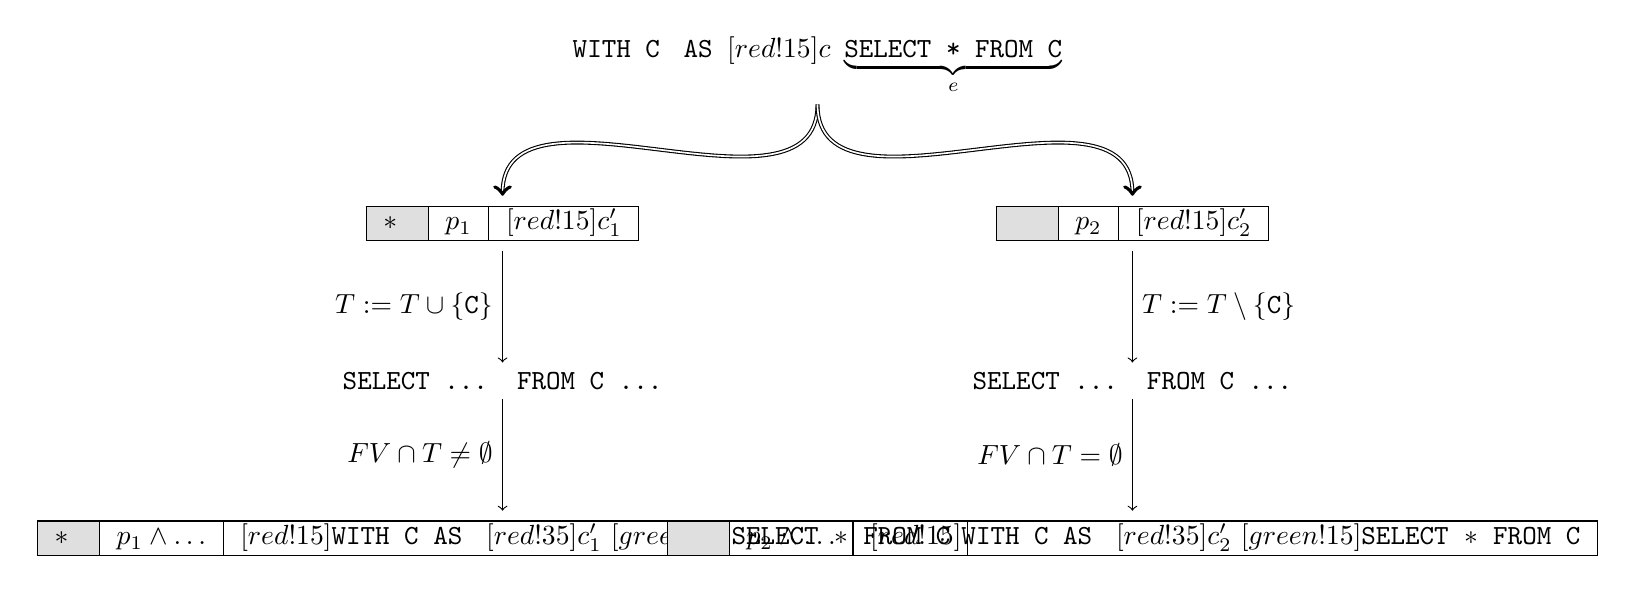
\begin{tikzpicture}
    \node (cte) at (4, 1) {\texttt{WITH C} \AS $\highlight[red!15]{c}~ \underbrace{\texttt{SELECT * FROM C}}_e$};
    \node (cte1) at (0, -1) {
        \begin{tabular}{|p{1em}|r|c|}\hline
        \cellcolor{gray!25} $\ast$ & $p_1$ & $\highlight[red!15]{c'_1}$\\\hline
        \end{tabular}
    };
    \node (cte2) at (8, -1) {
        \begin{tabular}{|p{1em}|r|c|}\hline
        \cellcolor{gray!25} & $p_2$ & $\highlight[red!15]{c'_2}$\\\hline
        \end{tabular}
    };
    \node (select1) at (0, -3) {\texttt{SELECT ... FROM C ...}};
    \node (select2) at (8, -3) {\texttt{SELECT ... FROM C ...}};
    \node (r1) at (0, -5) {
        \begin{tabular}{|p{1em}|r|c|}\hline
        \cellcolor{gray!25} $\ast$ & $p_1 \land \hdots$ & $\highlight[red!15]{\texttt{WITH C AS } ~\highlight[red!35]{c'_1}}~\highlight[green!15]{\SELECT~*~\texttt{FROM C}}$\\\hline
        \end{tabular}
    };
    \node (r2) at (8, -5) {
        \begin{tabular}{|p{1em}|r|c|}\hline
        \cellcolor{gray!25} & $p_2 \land \hdots$ & $\highlight[red!15]{\texttt{WITH C AS } ~\highlight[red!35]{c'_2}}~\highlight[green!15]{\SELECT~*~\texttt{FROM C}}$\\\hline
        \end{tabular}
    };
    \draw[->, double, out=270, in=90] (cte) to (cte1.north);
    \draw[->, double, out=270, in=90] (cte) to (cte2.north);
    \draw[->] (cte1.south) --node[left] {$T := T \cup \{\texttt{C}\}$} (select1);
    \draw[->] (cte2.south) --node[right]{$T := T \setminus \{\texttt{C}\}$} (select2);
    \draw[->] (select1) --node[left] {$FV \cap T \neq \emptyset$} (r1);
    \draw[->] (select2) --node[left] {$FV \cap T = \emptyset$} (r2);
    \end{tikzpicture}
    \caption{}
    \label{fig:my_label}
\end{figure}



\subsection{\RSELECT- and \RFROM-rule}


\begin{figure}\small
    \begin{minipage}[b]{.5\linewidth}
    \centering
    \sqlcode{snippets/fib_cte.sql}
    \subcaption{Fib with Ctes}\label{fib_cte_udf}
    \end{minipage}%
    \begin{minipage}[b]{.5\linewidth}
    \centering
     \begin{tikzpicture}
    \node[anchor=west] (s1) at (0, 0) {
        \begin{tabular}{|p{1em}|l|l|}\hline
        \cellcolor{gray!25}                         & \mintinline{sql}{TRUE AND} ~~ & ~~\mintinline{sql}{WITH C AS (SELECT 1)}\\
        \cellcolor{gray!25}\multirow{-2}{*}{} & \mintinline{sql}{n <= 2}   ~~ & ~~\mintinline{sql}{SELECT (SELECT P.i FROM P)}\\\hline
        \end{tabular}
    };
    \node[anchor=west, below=of s1] (s2) {
        \begin{tabular}{|p{1em}|l|l|}\hline
        \cellcolor{gray!25}                         & \mintinline{sql}{TRUE AND}   ~~ & ~~\mintinline{sql}{WITH C AS (SELECT 1)}\\
        \cellcolor{gray!25}                         & \mintinline{sql}{n <> 3 AND }~~ & ~~\mintinline{sql}{     S(i) AS (SELECT fib_cte3(n-2))}\\
        \cellcolor{gray!25}\multirow{-3}{*}{$\ast$} & \mintinline{sql}{NOT n <= 2} ~~ & ~~\mintinline{sql}{SELECT (SELECT T.i + S.i FROM S, T)}\\\hline
        \end{tabular}
    };
    \node[anchor=west, below=of s2] (s2) {
        \begin{tabular}{|p{1em}|l|l|}\hline
        \cellcolor{gray!25}                         & \mintinline{sql}{TRUE AND}      ~~ & ~~\mintinline{sql}{WITH C AS (SELECT 1)}\\
        \cellcolor{gray!25}                         & \mintinline{sql}{NOT n <> 3 AND}~~ & ~~\mintinline{sql}{     S(i) AS (SELECT 1)}\\
        \cellcolor{gray!25}\multirow{-3}{*}{$\ast$} & \mintinline{sql}{NOT n <= 2}    ~~ & ~~\mintinline{sql}{SELECT (SELECT T.i + S.i FROM S, T)}\\\hline
        \end{tabular}
    };
    \end{tikzpicture}
    \subcaption{Recursive scenarios}\label{fib_cte_scenarios}
    \end{minipage}
    \caption{}\label{fib_cte_translation}
\end{figure}





\iffalse OLD
$$\quad(\textsc{from})\inferrule{
    \exists i \in \{1, ..., n\}: T \vdash \hasCallsite(e_{f_i}) \\
    T[a_1 \mapsto \bot, ..., a_n \mapsto \bot] \vdash \neg \hasCallsite(e_s) \land \neg \hasCallsite(e_w) \\
    \forall i \in \{1, ..., n\}: T, \varnothing \vdash (\TRUE, t_i) \rightarrow (B_i, R_i)
}{
    T, \varnothing \vdash (p, \SELECT e_s \FROM t_1 \AS a_1 \otimes ... \otimes  t_n \AS a_n \WHERE e_w) \rightarrow \\\\
    {\begin{tabular}[b]{LLLL}
    (~~&\{&(&\SELECT p ~\AND~ p_1 ~\AND~ \cdots ~\AND~ p_n, \\
          &&&\SELECT e_s \FROM t'_1 \AS a_1 \otimes ... \otimes  t'_n \AS a_n \WHERE e_w ~~)\\
      && | &~((p_1, t'_1), ..., (p_n, t'_n)) \in \times_{\{i|1\leq i \leq n\}} B_i\}, \\
    &\{&(&\SELECT p_1 ~\AND~ \cdots ~\AND~ p_n, \\
       &&&\SELECT e_s \FROM t'_1 \AS a_1 \otimes ... \otimes  t'_n \AS a_n \WHERE e_w ~~)\\
       &&| &~ ((p_1, t'_1), ..., (p_n, t'_n)) \in \times_{\{i|1\leq i \leq n\}} (B_i \cup R_i), \exists t' \in \{t'_1, ..., t'_n\} : \hasCallsite(t')\})\\
    \end{tabular}}
}$$
\fi
$$\quad(\textsc{from})\inferrule{
    \exists i \in \{1, ..., n\}: \hasCallsite(T, e_{f_i}) \\
    \neg \hasCallsite(T, e_s)\\
    \neg \hasCallsite(T, e_w) \\\\
    \forall i \in \{1, ..., n\}: T, \varnothing \vdash (\TRUE, t_i) \rightarrow (B_i, R_i)
}{
    T, \varnothing \vdash (p, \SELECT~ e_s ~\FROM~ t_1 \AS a_1 \otimes ... \otimes  t_n \AS a_n ~\WHERE~ e_w) \rightarrow \\\\
    {\begin{tabular}[b]{LLLL}
    (~~&\{&(&\SELECT~ p ~\AND~ p_1 ~\AND~ \cdots ~\AND~ p_n, \\
          &&&\SELECT~ e_s ~\FROM~ t'_1 \AS a_1 \otimes ... \otimes  t'_n \AS a_n ~\WHERE~ e_w ~~)\\
      && | &~((p_1, t'_1), ..., (p_n, t'_n)) \in \times_{\{i|1\leq i \leq n\}} B_i\}, \\[6pt]
    &\{&(&\SELECT~ p_1 ~\AND~ \cdots ~\AND~ p_n, \\
       &&&\SELECT~ e_s ~\FROM~ t'_1 \AS a_1 \otimes ... \otimes  t'_n \AS a_n ~\WHERE~ e_w ~~)\\
       &&| &~ ((p_1, t'_1), ..., (p_n, t'_n)) \in \times_{\{i|1\leq i \leq n\}} (B_i \cup R_i), \exists t' \in \{t'_1, ..., t'_n\} : \hasCallsite(t')\}\\
    )\\
    \end{tabular}}
}$$

\subsection{\RCTE-rule: Collecting and analyzing CTE-Scenarios}
CTE-Scenarios are computed and dependencies for the scenarios are collected.
$$\quad(\textsc{cte})\inferrule{
    \hasCallsite(T, \WITH a_1 \AS t_1, ..., a_n \AS t_n~q)\\
    T, \varnothing \vdash (p, t_1) \rightarrow (B, R) \\
    ((B \times \{\bot\}) \cup (R \times \{\top\})) = \{(p'_{t_1}, t'_1, r_{i_1}), ..., (p'_{t_k}, t'_k, r_k)\} = X\\
    \forall (p'_t, t', r_i) \in X: T[a_1 \mapsto r_i], C[a_1: (t', p'_t, FV^+(t')] \vdash (p, \WITH a_2 \AS t_2, ..., a_n \AS t_n~q) \rightarrow (B_i, R_i)
}{
    T, C \vdash (p, \WITH a_1 \AS t_1, ..., a_n \AS t_n~q) \rightarrow ((\cup_{1 \leq i \leq k} B_i), (\cup_{1 \leq j \leq k} R_j)\})
}$$

$$\quad(\textsc{cte})\inferrule{
    T \vdash \hasCallsite(\WITH~ a_1 \AS t_1, ..., a_n \AS t_n~q)\\
    T, \varnothing \vdash (p, t_1) \rightarrow (B, R) \\
    \forall (p'_t, t') \in B: T \setminus \{a_1\}, C[a_1: (t', p'_t, FV^+(t')] \vdash (p, \WITH~ a_2 \AS t_2, ..., a_n \AS t_n~q) \rightarrow (B_i, R_i) \\
    \forall (p'_t, t') \in R: T \cup \{a_1\}, C[a_1: (t', p'_t, FV^+(t')] \vdash (p, \WITH~ a_2 \AS t_2, ..., a_n \AS t_n~q) \rightarrow (B_j, R_j)
}{
    T, C \vdash (p, \WITH~ a_1 \AS t_1, ..., a_n \AS t_n~q) \rightarrow ((\cup_{1 \leq i \leq k} B_i) \cup (\cup_{1 \leq j \leq l} B_j), (\cup_{1 \leq j \leq k} R_j) \cup (\cup_{1 \leq j \leq l} R_j)\})
}$$

\sqlcode{snippets/from_shadowing.sql}
\subsection{\RWITH-rule: Attaching used CTEs only}
When all CTEs at a level are processed, the actual query is processed independently. The query contains none of the preceeding CTEs anymore, so that it is sufficient to analyze the current subtree together with the set $T$ of recursive CTEs in scope to decide whether a subtree is recursive.
$$\quad(\textsc{with})\inferrule{
    C \neq \varnothing\\
    T, \varnothing \vdash (p, q) \rightarrow (B, R)
}{
    T, C \vdash (p, \WITH q) \rightarrow \\\\
    {\begin{tabular}[b]{LLLL}
    (~~&\{&(&\WITH [a_i \AS t_i]^{(a_i, t_i) \in \sigma_{a, t}(q'_{ctePreds})}~\SELECT (\AND_{p_i \in \{p_q\} \cup \sigma_p(q'_{ctes})} p_i), \\
          &&&\WITH [a_i \AS t_i]^{(a_i, t_i) \in \sigma_{a, t}(q'_{ctes})}~~q'~\\
          &&| &~(p_q, q') \in B,~ q'_{ctes} = C[FV^+(q')],~ q'_{ctePreds} = C[\cup_{x_p \in \{p_q\} \cup \sigma_p(q'_{ctes})} FV^+(x_p)]\},\\
    &\{&(&\WITH [a_i \AS t_i]^{(a_i, t_i) \in \sigma_{a, t}(q'_{ctePreds})}~\SELECT (\AND_{p_i \in \{p_q\} \cup \sigma_p(q'_{ctes})} p_i), \\
    &&&\WITH [a_i \AS t_i]^{(a_i, t_i) \in \sigma_{a, t}(q'_{ctes})}~~q'~\\
    &&|&~(p_q, q') \in R,~ q'_{ctes} = C[FV^+(q')],~ q'_{ctePreds} = C[\cup_{x_p \in \{p_q\} \cup \sigma_p(q'_{ctes})} FV^+(x_p)])
    \end{tabular}}
}$$
\\

% REF
$$\quad(\textsc{ref})\inferrule{
   \text{isReference}(S) \\
   T \vdash \hasCallsite(S)
}{
    T, C \vdash (p, S) \rightarrow (\{\}, \{(p, S)\})
}$$


\section{Postprocessing of the scenarios}
\subsection{Extraction of callsite-arguments}
We need to extract the arguments of the callsites within a recursive case, eg: 
\begin{minted}{sql}
SELECT T.a + T.b + T.c FROM (SELECT f(n-1, 2), 3, 4 + f(5, 6) FROM T WHERE p) AS T(a, b, c)
\end{minted}
into a set of callsite-arguments with its arguments $\{(\SELECT n-1, \SELECT 2), (\SELECT 5, \SELECT 6)\}$. As we require the callsite-arguments to be uncorrelated, we do not have to deal with references to \FROM but only to CTEs, wich simplifies things greatly.

Remove sourrinding query if callsite is within \SELECT, because the value of the callsite-arguments must be invariant to the tables references in \FROM.
$$\quad(\textsc{select})\inferrule{
    \exists i \in \{1, ..., n\}: \text{containsCallsite}(s_i) \\
    \forall i \in \{1, ..., n\}: \varnothing \vdash s_i \rightarrow P_i
}{
    \varnothing \vdash \SELECT s_1, ..., s_n \FROM f \WHERE w \rightarrow \\\\
    \{(\SELECT e_1, ..., \SELECT e_k) | (e_1, ..., e_k) \in \cup_{i \in \{1, ..., n\}} P_i \}
}$$

Remove outer query if callsite is within FROM, because sourrounding query is irrelevant for evaluation of subqueries in FROM.
$$\quad(\textsc{from})\inferrule{
    \forall i_j \in \{i_1, ...., i_m\} \subseteq \{1, ..., n\}: \text{containsCallsite}(f_{i_j})\\
    \forall i_j \in \{i_1, ...., i_m\}: \varnothing \vdash f_{i_j} \rightarrow P_{i_j}
}{
    \varnothing \vdash \SELECT s \FROM a_1 \AS f_1 \otimes ... \otimes a_n \AS f_n \WHERE w \rightarrow \cup_{i \in \{1, ..., n\}} P_i
}$$

Evaluate CTEs seperately, keeping previous CTEs that are referenced, in the case that there are callsites inside CTEs. Saving also every CTE to the CTE-store if they are references form the actual query.
$$\quad(\textsc{cte})\inferrule{
    \varnothing \vdash t_1 \rightarrow P \\
    C[a_1 : (t_1, FV^+(C, t_1))] \vdash \WITH a_2 \AS t_2, ..., a_n \AS t_n ~q \rightarrow P_w
}{
    C \vdash \WITH a_1 \AS t_1, ..., a_n \AS t_n ~q \rightarrow \\\\
    \{(\WITH [a_i \AS t_i]_{(a_i, t_i) \in C[FV^+(e_1)]} ~e_1, ..., \WITH [a_i \AS t_i]_{(a_i, t_i) \in C[FV^+(e_m)]} ~e_m) | (e_1, ..., e_m) \in P\} \cup P_w
}$$


$$\quad(\textsc{with})\inferrule{
    \varnothing \vdash q \rightarrow P
}{
    C \vdash \WITH q \rightarrow \\\\
    \{(\WITH [a_i \AS t_i]_{(a_i, t_i) \in C[FV^+(e)]} ~e_1, ..., \WITH [a_i \AS t_i]_{(a_i, t_i) \in C[FV^+(e_m)]} ~e_m) | (e_1, ..., e_m) \in P\}
}$$

Remove surrounding expression for every branch that contains a callsite, collecting results of all arguments.
$$\quad(\textsc{expr})\inferrule{
    \exists i \in \{1, ...., n\}: \text{containsCallsite}(e_i)\\
    \forall i \in \{1, ...., n\}: \varnothing \vdash e_i \rightarrow P_i
}{
    \varnothing \vdash \text{expr}(e_1, e_2, ..., e_n) \rightarrow \cup_{i \in \{1, ...., n\}} P_i
}$$

Remove recursive call and collect args.
$$\quad(\textsc{call})\inferrule{
}{
    \varnothing \vdash fn_{rec}(e_1, e_2, ..., e_n) \rightarrow \{ (e_1, e_2, ..., e_n) \}
}$$

If subbranch contains no callsite, stop and return empty set.
$$\quad(\textsc{nocall})\inferrule{
\neg \text{containsCallsite}(e)
}{  
    \varnothing \vdash e \rightarrow \{\}
}$$

Callsites within aggregate-functions are forbidden by the restriction that there must be a static number of callsites. Looping through a table, evaluating a recursive call per row is not allowed.



\chapter{Query templates}
% Evaluation of recursive functions
The translated functions follow all a common schema in general. First, the callstack-graph is created, top-down until the basecases are reached. The basecases are then evaluated with the according arguments discovered by the callgraph. Evaluation continues bottom-up as new recursive cases have results of their callsites available.

% Two phases: Callgraph growth and callstack evaluation
This two phases, callstack discovery and callstack evaluation, are implemented by two CTEs, \texttt{callstack} and \texttt{evaluation}. The final query selects the desired final output from the evaluation-CTE. \autoref{fig:standard_template_structure} illustrates the very high level idea of the standard translation template.

\begin{figure}[h!]
    \centering
    \sqlcode{snippets/template_structure.sql}
    \caption{High-level structure of the standard query template (simplified).}
    \label{fig:standard_template_structure}
\end{figure}

% Special care needs to be taken to behave not only in terms of result values, but also in terms of termination.
Special care needs to be taken to behave like the original function in terms of termination. Call-loops in the original function lead to an infinite growing callstack, causing nontermination. By using memoization in the translation, this does not happen in our template, so we have to detect that case and manually init nontermination.

In this chapter I will provide a number of "macros" that fill the templates with values. I give these macros with respect to the running example of \texttt{fib}, so for a function with a single attribute. This avoids cluttering difficult spots with excessiv notation. To generalize to more attributes the following things need to be done:
\begin{itemize}
    \item Instead of a single column \texttt{in\_1} or \texttt{out\_1}, we need further columns \texttt{in\_2, ..., in\_n} and \texttt{out\_2, ..., out\_n}.
    \item Whenever we match tables by their arguments, eg. \texttt{(c.in\_1) = (e.out\_1)} it is clear that this needs to be altered analogous to \texttt{(c.in\_1, c.in\_2, ..., c.in\_n) = (e.out\_1, e.out\_2, ..., out\_n)}.
    \item The same applies whenever replacing UDF arguments: \texttt{q[x1/\$1]} needs to become \texttt{q[x1/\$1, x2/\$1, ..., xn/\$n]}.
\end{itemize}
For full examples with more than one argument see the appendix. 

\section{Callgraph discovery}

The idea of the callgraph-CTE is to utilize the generated predicates from the recursive scenarios to detect which callsites in the original query are reached with the arguments of the current invocation.
Starting with the original arguments of the UDF-invocation the applicable scenario is detected and the contained callsites are discovered. The arguments passed to the newly discovered callsites are evaluated independetly and used to recursively collect subsequent calls.

\subsection{Tabular callgraph representation}

\begin{figure}[h!]\small
    \begin{minipage}[b]{.5\linewidth}
    \centering
    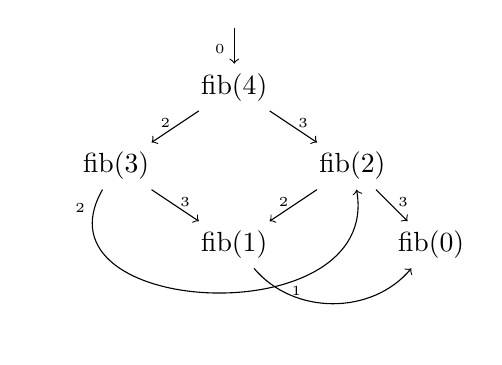
\begin{tikzpicture}
% nodes
\node (f4)     at (2.5, 2) {fib(4)};
    \node (f3) at (1, 1) {fib(3)};
        \node (f1) at (2.5, 0) {fib(1)};
    \node (f2) at (4, 1) {fib(2)};
        \node (f0) at (5, 0) {fib(0)};
% arrows
\draw[<-] (f4) -- node[pos=0.4, left, label distance=5mm]{\tiny{0}} +(0, 0.75);

\draw[->] (f4) -- node[pos=0.4, left, label distance=5mm]{\tiny{2}} (f3);
\draw[->] (f4) -- node[pos=0.4, right, label distance=5mm]{\tiny{3}} (f2);

    \draw[->, bend right=100, out=240, looseness=1.5] (f3) to node[pos=0.05, left, label distance=5mm]{\tiny{2}} (f2);
    \draw[->] (f3) -- node[pos=0.4, right, label distance=5mm]{\tiny{3}} (f1);
    \draw[->] (f2) -- node[pos=0.4, left, label distance=5mm]{\tiny{2}} (f1);
        \draw[->, bend right=50] (f1) to node[pos=0.2, right, label distance=5mm]{\tiny{1}} (f0);
    \draw[->] (f2) -- node[pos=0.4, right, label distance=5mm]{\tiny{3}} (f0);
\end{tikzpicture}
    \subcaption{Callgraph during execution}\label{fig:fib_callstack_graph}
    \end{minipage}%
    \begin{minipage}[b]{.5\linewidth}
    \centering
     
    \begin{tabular}{c|c|c}
        \texttt{in\_arg\_1} & \texttt{callsite} & \texttt{call\_arg\_1} \\
        \hline
        \hline
        \texttt{NULL} & \texttt{0} & \texttt{4}\\
        \texttt{4} & \texttt{2} & \texttt{3}\\
        \texttt{4} & \texttt{3} & \texttt{2}\\
        \hline
        \hline
        \texttt{3} & \texttt{2} & \texttt{2}\\
        \texttt{3} & \texttt{3} & \texttt{1}\\
        \texttt{2} & \texttt{2} & \texttt{1}\\
        \texttt{2} & \texttt{3} & \texttt{0}\\
        \hline
        \texttt{1} & \texttt{1} & \texttt{0}\\
        \hline
    \end{tabular}
    \subcaption{Tabular representation of the callstack}\label{fig:fib_callstack_table}
    \end{minipage}
    \caption{Callgraph of \texttt{fib(4)} (a) and its tabular representation as generated by the \texttt{callstack}-CTE (b). Each edge represents a callsite.}\label{fig:fib_callstack}
\end{figure}

The callstack-CTE creates a direct encoding of the callstack graph (\autoref{fig:fib_callstack}). Each row depicts an edge between two nodes, including the label. Nodes of the callgraph correspond to recursive invocations, identified by their arguments, one column per argument. Beside arguments of the caller and callee, the id of the callsite is noted. Callsite ids are used to associate callsites to scenarios.

\subsection{Collecting callsite arguments}

Thanks to the data from the scenario analysis, the query to add the rows for new callsite can be generated by a simple macro (\autoref{marco:collect_call_maybe}). The predicate acts as guard to add only callsites of the appropriate evaluation scenario. Only if the predicate is fulfilled, any row is returned. The third row in \autoref{fig:fib_callstack_table} is eg. generated by \mintinline{postgresql}{<collect_call_maybe(d.out_1, p1, <callsite id: 2, arg_1: (SELECT $1 - 2)>)>}.

\begin{figure}[h!]\centering
    \begin{minted}{postgresql}
    <collect_call_maybe(in_arg_1, predicate, callsite)>
        := SELECT
             in_arg_1                    AS in_1, 
             callsite.id                 AS callsite_id,
             callsite.arg_1[in_arg_1/$1] AS out_1
           FROM predicate AS p(is_true)
           WHERE p.is_true
    \end{minted}
  \caption{Pseudocode to generate a single call to the callgraph-table. $q[y/x]$ denots the operation of replacing y for x in q. For \texttt{in\_arg\_1} it is used in the beginning \$1 and later references to preceding arguments from the table.}
  \label{marco:collect_call_maybe}
\end{figure}

The macro from \autoref{marco:collect_call_maybe} creates only a query, returning one or none rows. To collect \textit{all} callsites, the query needs to test all callsites of all scenarios (\autoref{macro:collect_calls}). As all callsites within a scenario depend on the same predicate, the scenario-predicate can be pulled up into a CTE to avoid multiple evaluations.

\begin{figure}[h!]\centering\small
    \begin{minted}{postgresql}
    <collect_calls(in_arg_1, scenarios)> :=
        WITH p1 AS (scenarios[1].predicate)[in_arg_1/$1],
             p2 AS (scenarios[2].predicate)[in_arg_1/$1]
             
        -- Scenario 1
        (   -- Callsite 1
            <collect_call_maybe(in_arg_1, p2, scenarios[2].callsites[1])>   )
        
        UNION
        
        -- Scenario 2
        (   -- Callsite 2
            <collect_call_maybe(in_arg_1, p1, scenarios[1].callsites[1])>
          UNION
            -- Callsite 3
            <collect_call_maybe(in_arg_1, p1, scenarios[1].callsites[2])>   )
\end{minted}
  \caption{All callsites of all scenarios needs to be tested to cover the entire function.}
  \label{macro:collect_calls}
\end{figure}

With the query generated by \texttt{<collect\_calls(\$1, scenarios)>} all callsites of the initial UDF invocation are obtained. Subsequent levels of the callgraph can be collected recursively by using the \texttt{out\_1}-column from the previous iteration instead of \texttt{\$1}. For each callsite from the previous iteration, the according evaluation scenario needs to be detected to collect new callsites. This for-each behaviour is implemented by \texttt{LATERAL} in the marco for \texttt{callgraph}.

\begin{figure}[h!]\centering
\begin{minted}{postgresql}
<callstack(rec_scenarios)> :=
  (
    (SELECT NULL, 0, $1) -- add original call
      UNION ALL
    <collect_calls($1, rec_scenarios)> 

  ) UNION (
    SELECT
      new_calls.*
    FROM
      callstack AS c, LATERAL (
        <collect_calls(c.out_1, rec_scenarios)>
      ) AS new_calls
  )
\end{minted}
  \caption{}
  \label{}
\end{figure}

For a complete example of the \texttt{callgraph}-CTE for fib, see \autoref{fib:callstack_cte_complete} in the appendix.

Callgraph growth ends as soon as no recursive scenario is applicable for any newly discovered callsites, ie. all callsites lead to basecases. In this case, the new iteration contains no rows, making \texttt{WITH RECURSIVE} stop.

\section{Callgraph evaluation}
% Evaluation starts bottom up at the leaves of the callstack
Evaluation starts bottom up from the leafs of the callgraph. Scenarios are evaluated by replacing their original arguments with references to the arguments from the callgraph (\autoref{macro:single_basecase}). Scenarios may depend on other scenarios that need to be evaluated first. If all dependencies of a scenario are evaluated, the scenario can be evaluated itself. Nonrecursive scenarios have no dependencies by definition and can be evaluated therefore straight ahead. From this initial rows evaluation continues. Finally, the desired result can be selected.

\begin{figure}[h!]\small
    \begin{minipage}[b]{.45\linewidth}
    \centering
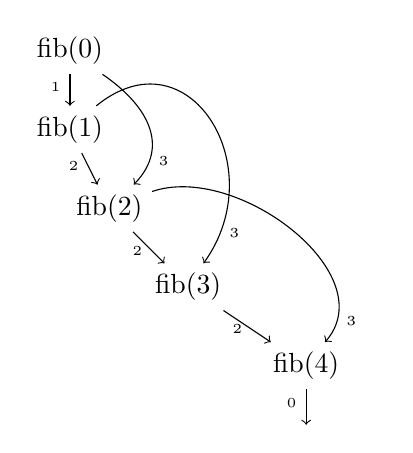
\begin{tikzpicture}
% nodes
\node (n4) at (2.5, -2) {fib(4)};
\node (n3) at (1, -1) {fib(3)};
\node (n2) at (0, 0) {fib(2)};
\node (n1) at (-0.5, 1) {fib(1)};
\node (n0) at (-0.5, 2) {fib(0)};
% arrows
\draw[->] (n0)     to node[pos=0.4,left] {\tiny{1}} (n1);
\draw[->, bend left=40, looseness=1.2, in=120] (n0)     to node[pos=0.8,right] {\tiny{3}} (n2);
\draw[->] (n1)     to node[pos=0.4,left] {\tiny{2}} (n2);
\draw[->, bend left=70, looseness=1.6, out=95] (n1)     to node[pos=0.9,right] {\tiny{3}} (n3);
\draw[->] (n2)     to node[pos=0.6,left] {\tiny{2}} (n3);
\draw[->, bend left=60, looseness=1, in=90] (n2)     to node[pos=0.9,right] {\tiny{3}} (n4);
\draw[->] (n3)     to node[pos=0.6,left] {\tiny{2}} (n4);
\draw[->] (n4)     to node[pos=0.4,left] {\tiny{0}} +(0, -0.75);
\end{tikzpicture}
    \subcaption{}\label{}
    \end{minipage}%
    \hfill
    \begin{minipage}[b]{.45\linewidth}
    \centering
    \begin{tabular}{c|c}
        \texttt{in\_arg\_1} & \texttt{result}\\
        \hline
        \hline
        \texttt{0} & \texttt{0}\\
        \hline
        \hline
        \texttt{1} & \texttt{1}\\
        \hline
        \texttt{2} & \texttt{1}\\
        \hline
        \texttt{3} & \texttt{2}\\
        \hline
        \texttt{4} & \texttt{3}\\
        \hline
    \end{tabular}
    \subcaption{}\label{fig:fib_callstack_cte}
    \end{minipage}
    \caption{a) Dependency-graph, directly retrieved from the callgraph. Callsite ids are annotated to the edges. Leafs are callsites resulting in basecases. b) \texttt{evaluation}-table that holds results for all evaluated scenarios. The first row is the result of the basecase. Following rows are computed iterativly.}\label{}
\end{figure}

\subsection{Evaluating nonrecursive scenarios}
Arguments for the evaluation of nonrecursive scenarios can be found in the leafs of the callgraph.
Evaluation of a single scenario is rather simple. UDF-arguments like \texttt{\$1} are replaced by references to arguments from the callgraph. The predicate from the generated scenario is evaluated in the \texttt{WHERE}-clause and prevents evaluation of wrong scenarios. \autoref{macro:single_basecase} shows a macro for evaluating a single scenario. Each scenario corresponds to a single query returning one or no rows. To collect all scenarios the union of this queries is built.
\begin{figure}[h!]
    \centering
    \begin{minted}{postgresql}
<evaluate nonrecursive scenario(scenario)>
 := SELECT c.out_1                    AS in_1, 
           scenario.query[c.out_1/$1] AS result
    FROM calls_to_basecase c
    WHERE scenario.predicate[c.out_1/$1]
    \end{minted}
    \caption{Macro for nonrecursive scenario evaluation.}
    \label{macro:single_basecase}
\end{figure}

For efficiency, nodes of recursive scenarios are filtered from the callgraph (resulting in CTE \texttt{calls\_to\_basecase}) as they cannot belong to basecases. If a callsite with argument \texttt{out\_1} can be found as input argument \texttt{in\_1} in the callgraph, then \texttt{out\_1} belongs to a recursive scenario. Graphically speaking, the query selects nodes of the callgraph with no outgoing edges, namely leafs, which represents callsites that leads to basecases.

\begin{figure}[h!]
    \centering
    \begin{minted}{postgresql}
<basecases(scenarios)> := 
   WITH calls_to_basecase(out_1) AS (
       SELECT DISTINCT out_1 
       FROM callgraph AS c
       WHERE NOT EXISTS (SELECT NULL FROM callgraph AS c2
                         WHERE c2.in_1 IS NOT DISTINCT FROM c.out_1)
   )
   <evaluate scenario(scenario[1], calls_to_basecases)>
     UNION ALL 
   <evaluate scenario(scenario[2], calls_to_basecases)>
    \end{minted}
    \caption{\texttt{basecase}-CTE.}
    \label{macro:basecases}
\end{figure}

The awkward \texttt{WHERE}-clause stirs from two issues. First, \texttt{IS NOT DISTINCT FROM} is the SQL-way of writing a simple \textit{=} while considering \mintinline{postgresql}{NULL=NULL} as true. This is required since \texttt{NULL} can be an argument of a callsite and needs to be matched with its result-row - tri-state logic hinders that. The \texttt{NOT EXISTS} comes from the fact that the simpler \texttt{NOT IN} is executed for every row as a subquery while \texttt{NOT EXISTS} is executed as a much more efficient antijoin. If disregarding this two issues, the \texttt{WHERE}-clause could be written easier to understand as \mintinline{postgresql}{c.out_1 NOT IN (SELECT c2.in_1 FROM callgraph c2)}.


\subsection{Recursive scenario evaluation}
The evaluation of recursive scenarios follows the schema of the evaluation of nonrecursive scenarios, but is a bit more involved. Callsite-results must be collected per scenario to decide if the scenario is evaluable yet. Only if all callsites of a scneario are evaluated, the scenario can be evaluated itself.

This operation resembles relational divsion $\texttt{S} \div \texttt{R}$: When dividing \texttt{S} by \texttt{R}, table \texttt{S} is grouped by the attributes that are not involved as join-attributes with \texttt{R}. The grouped columns from \textit{S} are returned, if every row in the group have found a join-partner from \texttt{S}. By dividing \texttt{callgraph} by \texttt{evaluation} (projecting away \texttt{callgraph.call\_site\_id}), we obtain only those input arguments that are evaluable, ie. have all required callsite-results available.

\begin{wrapfigure}{r}{0.6\textwidth}
  \sqlcode{snippets/relational_division.sql}
  \caption{Selecting available callsite-results per scenario using relational division with \texttt{array\_agg}. Does not play well with array-arguments.}
  \label{relational_division}
\end{wrapfigure}

The difficulty is to collect those callsite-results. The intuitive approach is to add an \texttt{array\_agg(e.result)} to the relational division (\autoref{relational_division}) that collects the results per scenario. This works well as long as we do not allow arrays as arguments: \texttt{array\_agg} require all input arrays to have the same dimensionality.

The solution is to avoid array aggregation and to "pivot" the groups instead: each callsite-result gets its own column. Pivoting is implemented by using Window-Functions and Partitions together with \texttt{nth\_value} instead of \texttt{GROUP BY} and \texttt{array\_agg}. This way, we circumvent any constraints regarding arrays and avoid expensive aggregation.

\vspace{5mm}

With this problem solved, evaluating a recursive scenario boiles down to replacing UDF-arguments and callsites with \texttt{callgraph}- resp. \texttt{evaluation}-references, similar to the evaluation of nonrecursive scenarios (\autoref{macro:single_basecase}). \autoref{macro:recursive_scenario_evaluation} gives a macro to evaluate a scenario utilizing the pivoting approach from above.

\begin{figure}[h!]\small
    \centering
    \begin{minipage}[b]{\linewidth}
    \centering
    \sqlcode{snippets/eval_recursive_scenario.sql}
    \vspace{3mm}
    \subcaption{(b) shows the result of the join, (c) the final result of the generated query and the effects of the ~\WHERE-clauses are annnotated: \circled{1} Do not consider arguments already evaluated callsites. \circled{2} Only consider callsites of the given scenario we are about to evaluate. \circled{3} Only keep rows where all callsites have an result available.}\label{}
    \end{minipage}%
    \vspace{7mm}
    \begin{minipage}[b]{\linewidth}
    \centering
    \begin{tabular}{c|c|p{10cm}p{1em}p{1cm}|c}
      \multicolumn{3}{l}{$\overbrace{\rule{5.2cm}{0pt}}^{\texttt{callgraph}}$}  & ${}^{\bowtie}$ & \multicolumn{2}{l}{$\overbrace{\rule{2.8cm}{0pt}}^{\texttt{evaluation}}$} \\
      \texttt{c.in\_1}                        & \texttt{c.call\_site\_id}  & \multicolumn{3}{c|}{\texttt{c.out\_1 = e.in\_1}} & \texttt{e.res}                                         \\\hline
      \multirow{2}{*}{\color{gray}4}          & \color{gray}2              & \multicolumn{3}{c|}{\color{gray}3}               & \texttt{\color{gray}NULL} \\
                                              & \color{gray}3              & \multicolumn{3}{c|}{\color{gray}2}               & \color{gray}1             \\\hline
      \cellcolor{green!25}                    & \cellcolor{yellow!30}2     & \multicolumn{3}{c|}{2}                           & \cellcolor{blue!20}1             \\
      \cellcolor{green!25}\multirow{-2}{*}{3} & \cellcolor{yellow!30}3     & \multicolumn{3}{c|}{1}                           & \cellcolor{red!20} 1            \\\hline
      \multirow{2}{*}{\color{gray}2}          & \color{gray}2              & \multicolumn{3}{c|}{\color{gray}1}               & \color{gray}1             \\
                                              & \color{gray}3              & \multicolumn{3}{c|}{\color{gray}0}               & \color{gray}0             \\\hline
      \color{gray}1                           & \color{gray}1              & \multicolumn{3}{c|}{\color{gray}0}               & \color{gray}0             \\\hline
    \end{tabular}
    \subcaption{Callgraph table joined with evaluation table.}\label{}
    \end{minipage}%
    \vspace{7mm}
    \begin{minipage}[b]{\linewidth}
    \centering
    \begin{tabular}{rc|c|c|c}
          & \texttt{in\_1} & \texttt{call\_1} \footnotesize{\color{gray}(id: \colorbox{yellow!20}{2})}  & \texttt{call\_2} \footnotesize{\color{gray}(id: \colorbox{yellow!20}{3})} & \texttt{count} \\\cline{2-5}
         \circled{3}                          & \color{gray}\markForTikz{row1Start}{4} & \color{gray}\texttt{NULL}                  & \color{gray}1                     & \color{gray}\markForTikz{row1End}{1} \\\cline{2-5}
         & \cellcolor{green!25}3              & \cellcolor{blue!20}1 & \cellcolor{red!20}1 & 2                                                            \\\cline{2-5}
         \circled{1}                          & \color{gray}\markForTikz{row2Start}{2} & \color{gray}1                              & \color{gray}0                     & \color{gray}\markForTikz{row2End}{2} \\\cline{2-5}
         \circled{2}                          & \color{gray}\markForTikz{row3Start}{1} & \color{gray}1                              & \color{gray}0                     & \color{gray}\markForTikz{row3End}{1} \\\cline{2-5}
    \end{tabular}
    \DrawHLine[thick, opacity=0.5]{row1Start}{row1End}
    \DrawHLine[thick, opacity=0.5]{row2Start}{row2End}
    \DrawHLine[thick, opacity=0.5]{row3Start}{row3End}
    \subcaption{Result of the query. Rows filtered by \WHERE~ are striked through,}\label{}
    \end{minipage}%
    \caption{Collecting callsite results of for evaluation of a scenario. The result for \texttt{fib(3)} is beeing evaluated. Table (a) shows the result of the }\label{macro:recursive_scenario_evaluation}
\end{figure}

The self-reference in recursive CTEs contains only the rows from the previous iteration, which is a problem when evaluating. Take the evaluation of \texttt{fib} for example (see \autoref{fig:fib_callstack_graph}): Each recursive scenario depends on the results from the last (\texttt{fib(n-1)}) and the penultimate iteration (\texttt{fib(n-2)}). Standard recursive CTE-semantics allows only access to \texttt{fib(n-1)}.

To work around this restriction, the working table is added to the actual result-rows in each iteration. If we choose this approach, the working-table will be never empty, but an empty working-table is the stopping criterion for evaluation of the CTE. Therefore we need to manually take care of returning an empty table when evaluation should stop. To achieve this, the new rows are computed seperately in a CTE and guard also addition of the previous results. \autoref{macro:evaluation_cte}, that shows the final \texttt{evaluation}-CTE, implements this approach.

\begin{figure}[h!]
  \sqlcode{snippets/evaluation_cte.sql}
  \caption{High-level structure of the evaluation-CTE}\label{macro:evaluation_cte}
\end{figure}


\FloatBarrier
\subsection{Result collection and termination}

The previous section introduced the components required to start and continue evaluation of recursive scenarios. The final task is to select the result or to trigger an infinite loop if a setting is detected where the original UDF does not terminate, but the translation has.

There are two ways how a recursive function may not terminate: Infinite recursion and looping calls. Infinite recursion leads always to new calls, never reaching a basecase, the callgraph is infinite. Each new call results in a new, different row that is added to the callgraph-table (\autoref{fig:infinite_callstack}). In this case, the translation does not terminate correctly, as the original.

\begin{figure}[h!]\small
    \begin{minipage}[b]{.5\linewidth}
    \centering
    \begin{minted}{sql}
SELECT CASE WHEN n = 0 THEN 0
            ELSE f(n-2)
       END
    \end{minted}
    \subcaption{UDF-body of a function \texttt{f}}
    \label{fig:infinite_callstack_udf}\par\vfill
    \end{minipage}%
    \begin{minipage}[b]{.5\linewidth}
    \centering
    \begin{tabular}{c|c|c}
in\_n & callsite & param\_n \\\hline
3  & 1 &  1 \\
1  & 1 & -1 \\
-1 & 1 & -3 \\
-3 & 1 & -5 \\
$\vdots$ & $\vdots$ & $\vdots$
    \end{tabular}
    \subcaption{Callgraph of that function. Recursion without a basecase.}
    \label{fig:infinite_callstack_callstack}
    \end{minipage}
    \caption{The function misses its basecase if called with an odd number like 3 and does not terminate. Every call leads to a new, different recursive call as call-arguments grow towards infinity.}\label{fig:infinite_callstack}
\end{figure}

The other case is looping calls. Since we utilize memoization, redundant calls lead only to a single row in the callgraph-table and not to multiple identical rows. Thus, the callgraph-table is finite while the original callgraph is not. Therefore, our implementation would terminate while the original does not. To maintain the original UDf behaviour we need to detect this case and trigger an infinite loop manually.

\begin{figure}[h!]\small
    \begin{minipage}[b]{.45\linewidth}
    \centering
    \begin{minted}{sql}
SELECT CASE WHEN n = 0 THEN 0
            WHEN n = 2 THEN f(0)
            ELSE f(n % 2) + f(2)
       END
    \end{minted}
    \subcaption{}\label{fig:some_loop_udf}
    \end{minipage}%
    \begin{minipage}[b]{.3\linewidth}
    \centering
    \begin{tabular}{c|c|c}
in\_n & callsite & param\_n \\\hline
3 & 2 & 1 \\
3 & 3 & 2 \\
2 & 1 & 0 \\
1 & 2 & 1 \\
1 & 3 & 2
    \end{tabular}
    \subcaption{}\label{fig:some_loop_callstack}
    \end{minipage}
    \begin{minipage}[b]{.2\linewidth}
    \centering
    \begin{tabular}{c|c}
in\_n & result \\\hline
0 & 0 \\\hline
2 & 0 \\
    \end{tabular}
    \subcaption{}\label{fig:some_loop_evaluation}
    \end{minipage}
    \caption{a) UDF-body of a function \texttt{f} where only some part of the callstack causes a loop. b) The callstack is finit, due to memoization. c) Evaluation can start, because some basecases are present, but has not all results available to finish evaluation up to the original call-arguments \texttt{3}.}\label{fig:some_loop}
\end{figure}

How is this situation detectable? If at least one path in the callgraph contains a loop, this path have no basecase where evaluation could start and thus evaluation will stop eventually without having evaluated the root-node. There is no row in the \textit{evaluation}-CTE containing a result for the original UDF-arguments. Instead of returning an empty table, an infinite loop is triggered (\autoref{fig:some_loop}).


\begin{figure}[h!]
    \centering
    \sqlcode{snippets/result_collection.sql}
    \caption{}
    \label{macro:result_collection}
\end{figure}



\chapter{Optimizations}

If certain characteristics of an UDF can be detected, the optimized translation templates can be chosen that exploits this characteristics. This may either improve performance or enables us to implement work-arounds for settings where the original templates are not applicable otherwise.

To make these optimizations no change in the scenario analysis is required. Instead, based on its output, ie. the generated scenarios, additionally analysis steps are performed to gather information required to choose the best templates.



\section{Single Recursion}

\begin{wrapfigure}{r}{0.2\textwidth}
  \vspace{-20pt}\centering
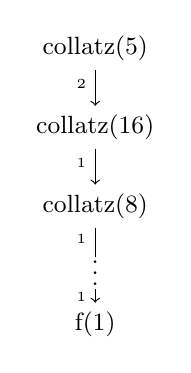
\begin{tikzpicture}\small
% nodes
\node (f1) at (0, 2) {collatz(5)};
\node (f2) at (0, 1) {collatz(16)};
\node (f3) at (0, 0) {collatz(8)};
\node (fn) at (0, -0.75) {$\vdots$};
\node (f0) at (0, -1.5) {f(1)};
% arrows
\draw[->] (f1) --node[pos=0.4, left, label distance=5mm]{\tiny{2}} (f2);
\draw[->] (f2) --node[pos=0.4, left, label distance=5mm]{\tiny{1}} (f3);
\draw (f3) --node[pos=0.4, left, label distance=5mm]{\tiny{1}} +(0, -0.65);
\draw[<-] (f0) --node[pos=0.4, left, label distance=5mm]{\tiny{1}} +(0, 0.45);
\end{tikzpicture}
  \vspace{-10pt}
  \caption{Callgraph of \texttt{collatz(5)}}
  \label{tr_callgraph}
\end{wrapfigure}

Single recursive functions have a linear branching behaviour (\autoref{tr_callgraph}). The function as a whole may contain multiple callsites as long as during evaluation each invocation will cause at most one recursive call. With the scenarios of the analysis, a single recursive function is quickly detected: If each scenario contains exactly one (or none) callsites, the function is single recursive.
The function that computed the length of the \textit{collatz-series} (\autoref{lst:collatz_udf}) is an example for a single recursive function.

\begin{figure}[h]
    \centering
    \begin{minipage}[b]{.45\linewidth}
    \centering
    \sqlcode{snippets/collatz.sql}
    \subcaption{UDf computing the length of the \textit{collatz-series} for a start number $\texttt{n} > 0$.}
    \label{lst:collatz_udf}
    \end{minipage}
    \begin{minipage}[b]{.5\linewidth}
    \centering\scriptsize
        \begin{tabular}{|p{1em}|p{3.3cm}|p{2.9cm}|}\hline
        \cellcolor{gray!25} & \texttt{\phantom{NOT }n=1} & \texttt{1}\\\hline
        \end{tabular}
        
        \begin{tabular}{|p{1em}|p{3.3cm}|p{2.9cm}|}\hline
        \cellcolor{gray!25} $\ast$ & \texttt{NOT n=1 AND \phantom{NOT }n \% 2 = 0} & \texttt{1 + collatz(n / 2)}\\\hline
        \end{tabular}
        
        \begin{tabular}{|p{1em}|p{3.3cm}|p{2.9cm}|}\hline
        \cellcolor{gray!25} $\ast$ & \texttt{NOT n=1 AND NOT n \% 2 = 0} & \texttt{1 + collatz(3 * n + 1)}\\\hline
        \end{tabular}
        \vspace{2em}
    \subcaption{Scenarios of \texttt{collatz}. Each recursive scenario contains just a single callsite.}\label{collatz_scenarios}
    \end{minipage}
    \caption{}
    \label{collatz_sql_with_scenarios}
\end{figure}

The evaluation happens thus also in a strict linear manner. As each scenario depends only on the result of the previous result, the work-around (see \autoref{macro:evaluation_cte}) to access all previous computed results becomes unnecessary. In each iteration exactly one result is computed and in the next iteration the dependant scenario will be evaluated. No need to add all previous results to the current result to have those rows later available (\autoref{opt_sr_evaluation_cte}). This has the very nice effect, that the intermediate-table of the \texttt{evaluation}-CTE does not grow quadratic (see \autoref{}) but only linear. Only actually new rows are added to the results.

\begin{figure}[h!]
    \centering
    \begin{minted}{postgresql}
WITH RECRUSIVE
    ...
    evaluation(in_1, res) AS (
        (TABLE basecases)
        
        UNION ( -- was UNION ALL
            WITH e AS (TABLE evaluation)
            (<evaluate recursive scenario_sr(scenario[1])>)
               UNION ALL
            (<evaluate recursive scenario_sr(scenario[2])>)
        )
    )
SELECT ...
    \end{minted}
    \caption{Simplified evaluation-template for single recursive UDFs.}
    \label{opt_sr_evaluation_cte}
\end{figure}

Furthermore, the rather complicated relational division, pivoting and filtering for evaluable scenarios (\autoref{macro:recursive_scenario_evaluation}) can be replaced by a much simpler query (\autoref{opt_sr_eval_scenario}). Because each scenario has only a single callsite, no grouping/partitioning is required to collect results of dependant callsites and to check whether all dependencies are available. If a result of the callsite is present, the scenario can be evaluated. What remains is basically a simple join (\autoref{opt_sr}).

\begin{figure}[h!]
    \centering
    \sqlcode{snippets/opt_sr.sql}
    \caption{Simplified macro for single recursive UDFs. Note how the \texttt{FROM}-clause is just a simple join and no \texttt{WHERE} is required anymore.}
    \label{opt_sr_eval_scenario}
\end{figure}





\section{Tail Recursion}
\begin{wrapfigure}{r}{0.5\textwidth}
  \vspace{-10pt}
    \sqlcode{snippets/collatz_tr.sql}
  \caption{Tail recursive formulation of \texttt{collatz}}
  \label{lst:fib_tr}
\end{wrapfigure}

A special form of single recursive functions are tail recursive functions. They do not have any evaluation context around any callsite so that each recursive scenario just returns another recursive call. Eventually, the result of the basecase is just passed all the way up in the callgraph to the root without any modifications. This last phase can therefore be skipped, which means that no \texttt{evaluation}-CTE is required.

The final result is present in the \texttt{basecase}-CTE. The basecase-CTE contains only a single value because single recursive functions have no branches in the callgraph (cp. \autoref{tr_callgraph}). The modifications on the template amount to removing the \texttt{evaluation}-CTE and changing result selection as shown in \autoref{tr_opt_template}. Furthermore the \texttt{callsite\_id}-column can be removed from the \texttt{callgraph}-CTE because the only use of the \texttt{callsite\_id} is to identify the corresponding scenario during evaluation (\autoref{marco:collect_call_maybe_optimized}).

\begin{figure}
    \centering
    \sqlcode{snippets/opt_tr.sql}
    \caption{Template for tail recursive UDFs. No \texttt{evaluation}-CTE is required anymore as all the basecases already return the final result.}
    \label{tr_opt_template}
\end{figure}


\begin{figure}[h!]\centering\small
    \begin{minted}{sql}
    <collect_call_maybe(in_arg_1, predicate, callsite)>
        := SELECT
             in_arg_1                    AS in_1, 
           --callsite.id                 AS callsite_id,
             callsite.arg_1[in_arg_1/$1] AS out_1
           FROM predicate AS p(is_true)
           WHERE p.is_true
    \end{minted}
  \caption{Pseudocode to generate a single call to the callstack-table, optimized for tail recursive UDFs. The callsite id is no longer required as the evaluation-phase is skipped.}
  \label{marco:collect_call_maybe_optimized}
\end{figure}

The detection if tail recursive functions happens again by inspecting the generated scenarios. The only callsite \texttt{f(...} must be present at the top level of the query of every scenario or nested arbitrarily deep in trivial \texttt{SELECT}s.
Nothing else may be present in the query as it would add a context that need to be saved and later on evaluated. Any computations like \texttt{1+(SELECT f(n))} would create a context around the call that need to be evaluated. The same for \FROM, even if the callsite-arguments contain no table-references, we are required to loop through the rows and create the output table.
\begin{figure}
    \centering
\begin{minted}{postgresql}
q := f(...)
q := (SELECT <c>)
q := (WITH [<alias> AS (<nonrecursive sql>), ...] <q>)
\end{minted}
    \caption{Grammar for tail-recursive queries. This notion could be extended, but catches most cases as it is.}
    \label{tr_grammar}
\end{figure}

CTEs are the only exception. If one of the callsite arguments reference a CTE and therefore the query is preceded by a \WITH-block, the function is still considered tail recursive. Callsite-arguments are evaluated during callgraph discovery. During evaluation the callsites, including their arguments, are replaced by references to their results. So, during evaluation, the CTEs are present but not used and could be therefore discarded. The resulting query is eligible for the tail recursive optimization.

\section{Constant parameter removal}

Unused parameters are always omitted.

Sometimes arguments are passed to functions that are invariant in subsequent calls, eg. configuration parameters. As these parameters do not change, it is not necessary to include them in the callgraph-table or to include them when matching rows by arguments. The argument can just be left as it is in the translation, eg. as \texttt{\$1}.

\begin{wrapfigure}{r}{0.66\textwidth}
  \vspace{-10pt}
    \sqlcode{snippets/sieve.sql}
  \caption{Sieve of Eratosthenes. \texttt{sieve(2, ARRAY[1, 2, 3, ..., n])} computes all prime numbers up to \texttt{n}.}
  \label{lst:sieve_udf}
\end{wrapfigure}

Removing unnecessary comparisons speeds up the query and saves memory as the same value is not copied again and again. The speedup can be significant, eg. in the function \texttt{sieve} (\autoref{lst:sieve_udf}). The function implements the sieve of Erathostenes, which filters out all non-prime numbers from a number array.

No change to the template is necessary and detection of constant arguments is straight-forward. The input is just removed from the list of arguments so that the argument is "not seen" when the templates are filled. The nth argument of a UDF is constant if the nth argument in each callsite is just \texttt{\$n}.

\begin{figure}[h]
    \centering\footnotesize
    \begin{minipage}[b]{\linewidth}
    \centering
    \begin{tabular}{c|c|c|c|c}
         in\_1 & in\_2                                     & callsite\_id & out\_1 & out\_2                                  \\\hline
         2     & \mintinline{postgresql}{ARRAY[2, 3, ..., 7]} & 1            & 3      & \mintinline{postgresql}{ARRAY[2, 3, ..., 7]}\\
         3     & \mintinline{postgresql}{ARRAY[2, 3, ..., 7]} & 1            & 4      & \mintinline{postgresql}{ARRAY[2, 3, ..., 7]}\\
    \end{tabular}
    \subcaption{\texttt{callgraph}-CTE for \texttt{sieve} without optimization}
    \label{}
    \end{minipage}
    \vspace{5mm}
    \begin{minipage}[b]{\linewidth}
    \centering
    \begin{tabular}{c|c|c}
         in\_1 & in\_2                                     & result                                  \\\hline
         4     & \mintinline{postgresql}{ARRAY[2, 3, ..., 7]} & \mintinline{postgresql}{ARRAY[2, 3, 4, 5, 6, 7]}\\
         3     & \mintinline{postgresql}{ARRAY[2, 3, ..., 7]} & \mintinline{postgresql}{ARRAY[2, 3, 4, 5, 7]}\\
         2     & \mintinline{postgresql}{ARRAY[2, 3, ..., 7]} & \mintinline{postgresql}{ARRAY[2, 3, 5, 7]}\\
    \end{tabular}
    \subcaption{\texttt{evaluation}-CTE for \texttt{sieve} without optimization}
    \label{}
    \end{minipage}
    \caption{}
    \label{}
\end{figure}

\begin{figure}[h]
    \centering
    \begin{minipage}[b]{.45\linewidth}
    \centering
    \begin{minted}{postgresql}
SELECT
    c.out_1      AS in_1, 
    c.out_2      AS in_2, 
    1            AS callsite_id,
    c.out_1 + 1  AS out_1
    c.out_2      AS out_2
FROM pred_1 AS p(is_true)
WHERE p.is_true
    \end{minted}
    \subcaption{\texttt{collect\_call\_maybe} without optimization}
    \label{}
    \end{minipage}
    \hfill
    \begin{minipage}[b]{.45\linewidth}
    \centering
    \begin{minted}{postgresql}
SELECT
    c.out_1      AS in_1, 
    1            AS callsite_id,
    c.out_1 + 1  AS out_1
FROM pred_1 AS p(is_true)
WHERE p.is_true
    \end{minted}
    \subcaption{\texttt{collect\_call\_maybe} with constant parameter removed}
    \label{}
    \end{minipage}
    \caption{Collection of a single scenario inside the \texttt{callgraph}-CTE.}
    \label{}
\end{figure}

\begin{figure}
    \centering
    \begin{minted}{postgresql}
SELECT c.in_1                                  AS in_1, 
       (SELECT array_agg(T.v)
        FROM unnest($2) AS T(v)
        WHERE (T.v = c.in_1 OR T.v % c.in_1 <> 0)
          AND T.v = ANY((SELECT e.result)))       AS result
FROM calls_to_basecases c
WHERE (SELECT (2 * c.out_1) > (array_length($2, 1))
    \end{minted}
    \caption{Evaluation of a nonrecursive scenario of \texttt{sieve} inside the \texttt{basecases}-CTE with constant parameter removed: \texttt{\$2} is not replaced by \texttt{c.in\_2}.}
    \label{fig:my_label}
\end{figure}

\section{Handling unhashable types}
The limitation to require hashability on input arguments of the UDF can be lifted if we implement measures to work around this issues. This lead to a greater applicability but is not desirable in the general case where this costly workaround is not necessary.


Hashable arguments
Hashable return value
\newpage

%%
\chapter{Evaluation and discussion}\label{results_discussion}

To protected PostgreSQL-process against infinite recursion, the execution stack is limited in size. The default in PostgreSQL 10.6 (\texttt{max\_stack\_depth}) is set to 2MB and can be manually increased. The maximum stack size is capped by the settings of the Operating System.\\
The available working memory (\texttt{work\_mem}) specifies how much memory can be consumed by in-memory operations like sorting or hashing. If the memory is exceeded, temporary results are stored on disk. Per default the working memory is set to 2MB. \cite[p. 512 ff.]{psql}

To fully exploit the capabilities of each implementation variant, the stack size is set to 7680kB (the limit of the OS) and working memory to 512MB. This way the recursive variant will not be terminated (too) early and the translation should be able to perform all computations in memory.

Using auto\_explain to track execution slows down by ca. 25\%.


\section{Original vs Translated Fibonacci Function}

\begin{figure}[h]
    \centering
    \includesvg{plots/fib_orig_vs_trans}
    \caption{Run time of fibonacci function in various versions.}
    \label{fig:fib_times}
\end{figure}
Runtimes vary greatly between the original recursive implementation, the automatic translation and a third, manually optimized fibonacci function\footnote{From \url{https://wiki.postgresql.org/wiki/Fibonacci_Numbers}, accessed: 15/12/2018}. To represent the wide variety the plots are drawed with logarithmic scales.

The original implementation is faster for very small inputs as it has less overhead then the translation. Additionally, the first two (fib(\$n-1) and fib(\$n-2)) calls are inlined. Anyway, the runtime of the original function grows very fast, so that $fib(30)$ already takes minutes. The translated function on the other hand is much faster. Where the original takes minutes, the translation is finished under 10ms. Even for fib(1000) the call returns after around 2 seconds. Yet, the translation cannot keep up with the manually optimized function. The same input here yields an result after a few milliseconds. But even here the runtime grows strongly as the inputs gets even larger. Yet, other limitations finally stop computing even larger fibonacci numbers: Somewhere between fib(600000) and fib(700000) the numeric datatype (which can represent numbers up to 131072 digits \cite[p. 124 f.]{psql}) fails with an overflow. That said, the manual optimized implementation is "as good as we can get".

The plot shows nicely how the automatic translation is magnitudes faster as the functional implemented original -- but the manually optimized implementation is again magnitudes faster. This affirms our initial claim, that our automatic translation gives you an great instant speed-up. Where the naive implementation gets slow, you can use the translation and the run-time drops from minutes to milliseconds. Where the translation runs for minutes, nothing else remains and you have to manually optimize the function. 

\subsection{Degree of recursion, DP}

\begin{figure}[h]
    \centering
    \includesvg{plots/branchN_dp}
    \caption{Comparision of UDF \texttt{branchN} (see \autoref{udfs:branchN}).}
    \label{fig:branchN}
\end{figure}

\subsection{Degree of recursion, DQ}

\begin{figure}[h]
    \centering
    \includesvg{plots/branchN_dq}
    \caption{Comparision of UDF \texttt{branchN} (see \autoref{udfs:branchN}).}
    \label{fig:branchN}
\end{figure}


\subsection{Varying number of arguments}

\begin{figure}[h]
    \centering
    \includesvg{plots/paramN_noopt}
    \caption{Run time of a same function (see \autoref{udfs:paramN}) with varying argument numbers. The translations are run using the generic template, without optimizations.}
    \label{fig:paramN}
\end{figure}

\autoref{fig:paramN} looks surprising. The original functions perform all equally and much better than the translations. Even more interstingly, the UDF with just one argument performs worst. This behaviour is surprising as we would guess that a simpler functions performs better in the translation because there is less data to manage and jonining tables is easier.\\
A first idea is, that the additional arguments give the functions more selective join predicates. Yet, this cannot be the case as the additional arguments of the used functions are just the arguments passed to the function, so the values are equal for all calls.\\
The reason for the big difference lays in the join order of the evaluation, as the query plan reveals. The function with one argument and n=200 makes first a nested loops anti join to join \texttt{evaluation} (rows=500, actual=68) with \texttt{callgraph} (rows=1, actual=201). The result (rows=1, actual=100) is joined with an hash join with \texttt{evaluation} (rows=500, actual=101).\\
The UDF with four arguments has flipped the order of the joins: First a hash join between \texttt{evaluation} (rows=940, actual=102) and \texttt{callgraph} (rows=100, actual=201) happens. The result (rows=1, actual=101) is joined with a nested loop anti-join with \texttt{evaluation} (rows=940, actual=69).

The problem is caused by the wrong guess about the number of rows returned from the scan of \texttt{callgraph}. The plans (see \autoref{plan:paramN}) are identical except for scenario-evaluation. During scenario-evaluation the CTE \texttt{e} (proxying \texttt{evaluation}) is joined with \texttt{callgraph} two times: Once for finding callsites of evaluated calls and once to check if the result is not yet calculated. The planner assumes that only a single row is returned using the filter \texttt{c.callsite\_id IN (1)}. But the UDF has only a single callsite, therefore the predicate is not selective at all.\\
The plan for the function with a single argument uses a \textit{nested loop anti join} to join the (supposed) single row from \texttt{callgraph} with \texttt{evaluation}. Nested Loop Joins are  a good choice when one table is small, otherwise a hash join performs better. The other plan uses first a hash join and than the nested loop join. As result, the nested loop join is executed on a smaller table which explains the better run-time. The plan from the UDF with one argument performs a nested loop join on tables with 68 and 201 rows, while in the other plan the inputs are sized 69 and 101 rows.

Now to the observation that the original performs better than the translation. This can be explained by the property, that the given function is linear recursive. No branching occurs and no memoization can be exploited. The overhead of the translation is significant is such a case: The evaluation-CTE adds in each step all the previous results to the new result. The number of rows is therefore $(0 + 1) + (1 + 1) + (2 + 1) + \dots + (n + 1) = \frac{n(n+1)}{2}$ and thus in $O(n^2)$. With the translation, we have made a linear function quadratically. Note that the results were obtained with optimizations disabled. So there is hope, as we see in the next section comparing optimizations to their originals.

\subsection{Optimizations}

\begin{figure}[h]
    \centering
    \includesvg{plots/paramN_opts}
    \caption{Comparision of UDF \texttt{param4} (see \autoref{udfs:paramN}) with varying optimizations.}
    \label{fig:paramN}
\end{figure}

% When limiting stack size to 100kb, param1_tr(320) is the first argument where it dies with "stack depth limit exceeded". As the function is nearly as simple as it gets, is seems to be valid to assume as lower bound that SQL will consume 1/3 kB per layer on the callstack. With default OS settings of max of 8MB on my machine, this means a maximum recursion depth of not more than roughly 25000 layers.  


\begin{figure}
    \centering
    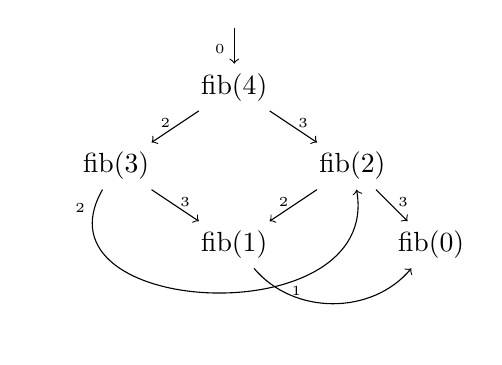
\begin{tikzpicture}
% nodes
\node (f4)     at (2.5, 2) {fib(4)};
    \node (f3) at (1, 1) {fib(3)};
        \node (f1) at (2.5, 0) {fib(1)};
    \node (f2) at (4, 1) {fib(2)};
        \node (f0) at (5, 0) {fib(0)};
% arrows
\draw[<-] (f4) -- node[pos=0.4, left, label distance=5mm]{\tiny{0}} +(0, 0.75);

\draw[->] (f4) -- node[pos=0.4, left, label distance=5mm]{\tiny{2}} (f3);
\draw[->] (f4) -- node[pos=0.4, right, label distance=5mm]{\tiny{3}} (f2);

    \draw[->, bend right=100, out=240, looseness=1.5] (f3) to node[pos=0.05, left, label distance=5mm]{\tiny{2}} (f2);
    \draw[->] (f3) -- node[pos=0.4, right, label distance=5mm]{\tiny{3}} (f1);
    \draw[->] (f2) -- node[pos=0.4, left, label distance=5mm]{\tiny{2}} (f1);
        \draw[->, bend right=50] (f1) to node[pos=0.2, right, label distance=5mm]{\tiny{1}} (f0);
    \draw[->] (f2) -- node[pos=0.4, right, label distance=5mm]{\tiny{3}} (f0);
\end{tikzpicture}
    \caption{Callgraph with memoization, The callstack-tree becomes a Directed Acyclic Graph (DAG). Each node represents an invocation and each outgoing edge a new callsite. Because of memoization, evaluation of equal invocations is performed only once, ie. they have the same descendants.}
    \label{fig:fib_callstack_memoization}
\end{figure}


\section{Advantages} Moimization, memory limitation, query planner
\section{Original vs. Translation}
\subsection{Number of recursive cases}
\subsection{Number of basecases}
\subsection{Number of parameters}
\subsection{Branching factor}

\section{Optimizations}
\subsection{Linear Recursion}
\subsection{Tail Recursive}
\subsection{Constant Parameters}

\section{Bottlenecks}
\newpage

%%
\section{Constraints of our approach}
Our approach can optimize a wide range of recursive UDFs, but there exist cases where a translation would not be beneficial or is not possible with my current implementation. I will characterize the set of translateable UDFs by formulating a number of constraints that must hold for a given query. Otherwise, the translation will fail or lead to an incorrect translation.
 
\subsection{No dependant callsites}
Our evaluation-strategy evaluates all callsites of an recursive expression independently and returns a result eventually only if all contained callsites have returned a result. For this reason, dependant callsites like $f(f(x))$ are not possible. Even more important is this constraint for \CASE-Statements. Imagine the following body of a recursive UDF \texttt{f}:
% TODO: Find more meaningful example
\begin{minted}{postgresql} 
SELECT CASE
  WHEN n      = 0 THEN 0
  WHEN f(n-1) = 0 THEN 1
  WHEN f(n-2) = 1 THEN 2
  ELSE 0
END;
\end{minted}
Here, the execution of the second \CASE-branch depends on the execution of the callsite in the first branch. After statically analysis, this block would result in one big recursive case with two callsites. The evaluation-strategy would execute both calls, leading to a behaviour possibly differing greatly from the original, eg. calling \texttt{f(n-2)} with invalid parameters leading to an infinite loop \texttt{(f(0), f(1)), (f(-1), f(-2), (f(-2), f(-3)), ...)}

\subsection{Explicit basecases required}
It is possible to write recursive functions that does not posses a basecase according to our static analysis, but do terminate and thus posses another way of terminating. Trivially, this can be achieved by using other conditionals as \CASE for case distinction like \texttt{GREATEST}, \texttt{LEAST}, \texttt{NULLIF} or \texttt{COALESCE}. Those functions can be viewed as syntactic sugar for \CASE since all of them can be formulated with \CASE only, see \ref{sql:cond_norm}. This could be done easilly in a normalizing preprocessing step.

But there exist more ways of formulating basecases which are harder do detect, like in the following example:
\sqlcode{snippets/no_basecases.sql}
Here, the basecase occurs when the table containing the recursive call is empty and therefore no recursive call happens. Examples like this show, that there is a variety of possibilities to write recursive functions without using an explicit \CASE. Translations for many of them may exist, but we focus in the following on recursive queries with explicit case-distinctions utilizing \CASE-expressions.

\subsection{Predicates and callsite-arguments may only reference CTEs and schema tables}
One challenge is slicing the function, the other is evaluating the arguments idependently from the surrounding query. While the first is mostly solved by my thesis, the latter is worth further examination to lift the constraints on callsite-arguments.

...

We require that predicates within a \texttt{CASE}-statement contain no references to row-varaibles like \texttt{T.v} that were introduced by an outer \FROM. This does not mean that no tables can be accessed. It is indeed possible to access tables, but these have to origin from an CTE, not a \FROM. This assumption is necessary to savely factor out the predicate which gets evaluated repeatably in the original implementation. This constraint can also be lifted if a table-compatible template is used for translation. The idea of the table-template is to replace all row variables by our own variables, alongside with the callsite-results. That way we have 
\sqlcode{snippets/predicates_must_be_selfcontained.sql}

The same goes for arguments of callsites.

\begin{listing}[ht]
\sqlcode{snippets/predicate_with_outside_references.sql}
\caption{Example of a (forbidden) predicate that has references to outside tables and thus returns a table of predicates.}
\label{lst:from_nonselfcontained}
\end{listing}
\newpage

%%
\input{4_Forschungsstand}
\newpage

%%
\chapter{Conclusion} \label{conclusion}

%%%%%%%%%%%%%%%%%%%%%%%%%
% Was war das Ziel?
% Was habe ich getan?
% Was wurde erreicht?
% Was lernen wir daraus?
% "Woran könnte man weiter forschen?"
%%%%%%%%%%%%%%%%%%%%%%%%%


Goal of this thesis was to automatically translate recursive SQL-UDFs into single, declarative queries. Recursive text-book style UDFs are easy to implement but trade performance for readability. One the other hand, manual optimizations are a time-consuming and challenging task that trades readability for performance. With the presented approach the programmer can keep writing recursive UDFs and translate them fully automatically into a optimized version.

The first step of the translation is the scenario analysis that slices the original UDF into its different evaluation scenarios. Each scenario-query is accompanied by a predicate that is used to detect the appropriate scenario for each call.

The analysis works already on a wide range for UDFs with a few constraints. The provided rules are able to create scenarios for nested W-S-F-W queries that use \texttt{CASE}-expressions as conditional. Callsites may be located in either the select-, from- or where-clause as well as in CTEs. Neither predicates nor callsites may contain row-references from the surrounding query, limiting the use of tables. An other notable constraint is that the evaluation of a callsite may not depend on the result of an other callsite.

Analysis and template filling are well separated steps, allowing to be extended easily in the future. Analysis rules are implemented very closely to the formal rules. The implementation of the templates is also modular, which makes it easy to replace parts of the templates or introduce new optimizations. The implementation for PostgreSQL has been tested with 30+ UDFs ranging from very simple functions up to complicated functions with more than 10 scenarios and nested CTEs.

The optimized translation performs better than the original for all tested UDFs, except for very tiny inputs. The translation performs automatic memoization, yielding to a speed-up by magnitudes for problems with overlapping subproblems. For divide-and-conquere algorithms the performance is improved by approximately factor 10. Yet, manual optimizations greatly outperform automatic translations as expected.

The provided optimizations has been shown to be useful, especially the template for single recursive functions. Without the optimization for single recursive functions, the estimates of the query planner lead to a plan that performs worse than the original UDF. Other optimizations speed-up evaluation by a fair constant factor.

There are two promising directions for future work: Widening the range of translateable functions or optimize evaluation by exploiting information from the callgraph. Allowing callsites to iterate through rows from a table would be a very useful improvement, especially as the motivation for this thesis is to make it more practical to perform computations near the data. Runtimes could be improved by harvesting and exploiting the information encoded in the callgraph.

\section*{Acknowledgements}
A number of people have supported me not only throughout this thesis, but my entire studies. Most notably my parents, who enabled me to studing in Tübingen and abroad and always encouraged me to slow down and learn "non scholae sed vitae".

I want to thank my supervisor, Christian Duta, for the very good support throughout my thesis. Thanks to Denis Hirn, who helped me unraveling the internals of PostgreSQL and provided a great library to generate ASTs from queries and pretty-printing them. Thanks to Prof. Grust to arouse my excitement about databases and functional programming in many great and memorable lectures. 
Many thanks to my girlfriend Ingrid Starnecker for the continuous support, especially during this thesis. Special thanks to my proofreaders Michael Lieberum and Johannes Jakubeit.
\newpage

%%
\cleardoublepage
\renewcommand{\thesection}{\Alph{section}}%
%\appendix 
%\addcontentsline{toc}{chapter}{Anhang} 

%%%%%%%%%%%%%%%%%%%%%%%%
%%%%%%%%%%%%%%%%%%%%%%%%
%%%%%%%%%%%%%%%%%%%%%%%%
\chapter[Appendix]{Appendix}
\phantomsection
\section{Examples of Rule application}
\subsection{\RWHEN-rule}
\begin{prooftree}
    \AxiomC{}\RightLabel{\scriptsize(base)}
    \UnaryInfC{\lstinputlisting{snippets/rules/fib/03-case-when.sql}}
    \AxiomC{}\RightLabel{\scriptsize(base)}
    \UnaryInfC{\lstinputlisting{snippets/rules/fib/03-case-then.sql}}
    \AxiomC{\vdots}\RightLabel{\scriptsize(else)}
    \UnaryInfC{\lstinputlisting{snippets/rules/fib/03-case-else.sql}}
    \RightLabel{\scriptsize(when)}
    \TrinaryInfC{\lstinputlisting{snippets/rules/fib/02-case.sql}}
\end{prooftree}


\section{Example translations}
\subsection{\texttt{fib}}
\begin{figure}
    \centering
    \sqlcode{snippets/fib_callstack.sql}
    \caption{\texttt{callstack}-CTE as standalone query. Note that the UDF argument \texttt{\$1} is replaced with a SQL-variable \texttt{:n}}
    \label{fib:callstack_cte_complete}
\end{figure}
\subsection{\texttt{gcd} without optimization}
\subsection{\texttt{gcd} with single recursion optimization}
\subsection{\texttt{gcd} with tail recursive optimization}
\subsection{\texttt{sieve} without optimization}
\subsection{\texttt{sieve} with constant argument removal}
\section{Conditional normalization}
\section{Usage of \texttt{twr}, a Haskell implementation for PostgreSQL}
\sqlcode{snippets/conditional_normalization.sql}\label{sql:cond_norm}
\section{Evaluation}
\begin{figure}
    \centering
    \sqlcode{appendix/paramN.sql}
    \caption{UDFs with varying number of arguments used for \autoref{fig:paramN}}
    \label{udfs:paramN}
\end{figure}
%%%%%%%%%%%%%%%%%%%%%%%%


%%%%%%%%%%%%%%%%%%%%%%%%%%%%%%%%%%%%%%%%%%%%%%%%%%%%%%%%%%%%%%%%%%%%%%%%%%%%%
%%% Bibliographie
%%%%%%%%%%%%%%%%%%%%%%%%%%%%%%%%%%%%%%%%%%%%%%%%%%%%%%%%%%%%%%%%%%%%%%%%%%%%%

\addcontentsline{toc}{chapter}{Bibliography}
\bibliographystyle{unsrt}
\bibliography{mylit}
%% Obige Anweisung legt fest, dass BibTeX-Datei `mylit.bib' verwendet
%% wird. Hier koennen mehrere Dateinamen mit Kommata getrennt aufgelistet
%% werden.

\cleardoublepage

%%%%%%%%%%%%%%%%%%%%%%%%%%%%%%%%%%%%%%%%%%%%%%%%%%%%%%%%%%%%%%%%%%%%%%%%%%%%%
%%% Erklaerung
%%%%%%%%%%%%%%%%%%%%%%%%%%%%%%%%%%%%%%%%%%%%%%%%%%%%%%%%%%%%%%%%%%%%%%%%%%%%%
\thispagestyle{empty}
\section*{Selbst\"andigkeitserkl\"arung}

Hiermit versichere ich, dass ich die vorliegende Masterarbeit 
selbst\"andig und nur mit den angegebenen Hilfsmitteln angefertigt habe und dass alle Stellen, die dem Wortlaut oder dem 
Sinne nach anderen Werken entnommen sind, durch Angaben von Quellen als 
Entlehnung kenntlich gemacht worden sind. 
Diese Masterarbeit wurde in gleicher oder \"ahnlicher Form in keinem anderen 
Studiengang als Pr\"ufungsleistung vorgelegt. 

\vskip 3cm

Ort, Datum	\hfill Unterschrift \hfill 

\end{document}